\documentclass[sigplan,10pt,anonymous,review]{acmart}
\renewcommand\footnotetextcopyrightpermission[1]{}
\settopmatter{printfolios=true}

\usepackage{booktabs}
\usepackage{subcaption}
\usepackage{xspace}
\usepackage{listings}
\usepackage{algorithm}
\usepackage[noend]{algpseudocode}
\usepackage{graphicx}
\usepackage{pifont}
\usepackage{multirow}
\usepackage{tikz}
\usepackage{stfloats}
\usetikzlibrary{positioning,fit,calc,arrows.meta,patterns}

\newcommand{\sys}{\textsc{Smash}\xspace}
\newcommand{\pp}{\%\xspace}
\newcommand{\punt}[1]{}
% Allow line breaks inside \texttt at underscores, camelCase boundaries, etc.
\newcommand{\tcode}[1]{\texttt{\hspace{0pt}#1}}
% Give LaTeX extra stretch to avoid marginal overfull hboxes
\emergencystretch=3pt

% Auto-generated macros from benchmark results (see gen_macros.py)
% Auto-generated from benchmark results. Do not edit by hand.
% Regenerate with: cd paper && python3 gen_macros.py
% Primary platform: linux


% ============================================================
% Platform: macos (suffix: Mac)
% ============================================================

% ── [Mac] Ablation results (per-app, per-config) ──
\newcommand{\ablSqliteBaselineRssRedMac}{25.8}
\newcommand{\ablSqliteBaselineRssRedIntMac}{26}
\newcommand{\ablSqliteBaselineFillRssMac}{565}
\newcommand{\ablSqliteBaselineServeRssMac}{571}
\newcommand{\ablSqliteBaselineMinRssMac}{1}
\newcommand{\ablSqliteBaselineCoolRssMac}{424}
\newcommand{\ablSqliteBaselineAucMac}{14263}
\newcommand{\ablSqliteBaselineOpsMac}{87427}
\newcommand{\ablSqliteDefaultRssRedMac}{75.5}
\newcommand{\ablSqliteDefaultRssRedIntMac}{76}
\newcommand{\ablSqliteDefaultFillRssMac}{452}
\newcommand{\ablSqliteDefaultServeRssMac}{154}
\newcommand{\ablSqliteDefaultMinRssMac}{0}
\newcommand{\ablSqliteDefaultCoolRssMac}{110}
\newcommand{\ablSqliteDefaultAucMac}{5452}
\newcommand{\ablSqliteDefaultOpsMac}{68025}
\newcommand{\ablSqliteDictRssRedMac}{72.9}
\newcommand{\ablSqliteDictRssRedIntMac}{73}
\newcommand{\ablSqliteDictFillRssMac}{452}
\newcommand{\ablSqliteDictServeRssMac}{167}
\newcommand{\ablSqliteDictMinRssMac}{0}
\newcommand{\ablSqliteDictCoolRssMac}{122}
\newcommand{\ablSqliteDictAucMac}{5848}
\newcommand{\ablSqliteDictOpsMac}{72588}
\newcommand{\ablSqliteNoArenasRssRedMac}{75.5}
\newcommand{\ablSqliteNoArenasRssRedIntMac}{76}
\newcommand{\ablSqliteNoArenasFillRssMac}{452}
\newcommand{\ablSqliteNoArenasServeRssMac}{193}
\newcommand{\ablSqliteNoArenasMinRssMac}{0}
\newcommand{\ablSqliteNoArenasCoolRssMac}{110}
\newcommand{\ablSqliteNoArenasAucMac}{5608}
\newcommand{\ablSqliteNoArenasOpsMac}{83410}
\newcommand{\ablSqliteLzFourOnlyRssRedMac}{75.5}
\newcommand{\ablSqliteLzFourOnlyRssRedIntMac}{76}
\newcommand{\ablSqliteLzFourOnlyFillRssMac}{452}
\newcommand{\ablSqliteLzFourOnlyServeRssMac}{193}
\newcommand{\ablSqliteLzFourOnlyMinRssMac}{0}
\newcommand{\ablSqliteLzFourOnlyCoolRssMac}{110}
\newcommand{\ablSqliteLzFourOnlyAucMac}{5600}
\newcommand{\ablSqliteLzFourOnlyOpsMac}{80325}
\newcommand{\ablSqliteNoZeroDeferRssRedMac}{75.5}
\newcommand{\ablSqliteNoZeroDeferRssRedIntMac}{76}
\newcommand{\ablSqliteNoZeroDeferFillRssMac}{452}
\newcommand{\ablSqliteNoZeroDeferServeRssMac}{155}
\newcommand{\ablSqliteNoZeroDeferMinRssMac}{0}
\newcommand{\ablSqliteNoZeroDeferCoolRssMac}{110}
\newcommand{\ablSqliteNoZeroDeferAucMac}{5528}
\newcommand{\ablSqliteNoZeroDeferOpsMac}{73529}
\newcommand{\ablSqliteNoPrefetchRssRedMac}{75.5}
\newcommand{\ablSqliteNoPrefetchRssRedIntMac}{76}
\newcommand{\ablSqliteNoPrefetchFillRssMac}{452}
\newcommand{\ablSqliteNoPrefetchServeRssMac}{194}
\newcommand{\ablSqliteNoPrefetchMinRssMac}{0}
\newcommand{\ablSqliteNoPrefetchCoolRssMac}{110}
\newcommand{\ablSqliteNoPrefetchAucMac}{5662}
\newcommand{\ablSqliteNoPrefetchOpsMac}{84528}
\newcommand{\ablSqliteSingleWorkerRssRedMac}{75.6}
\newcommand{\ablSqliteSingleWorkerRssRedIntMac}{76}
\newcommand{\ablSqliteSingleWorkerFillRssMac}{452}
\newcommand{\ablSqliteSingleWorkerServeRssMac}{170}
\newcommand{\ablSqliteSingleWorkerMinRssMac}{0}
\newcommand{\ablSqliteSingleWorkerCoolRssMac}{110}
\newcommand{\ablSqliteSingleWorkerAucMac}{5699}
\newcommand{\ablSqliteSingleWorkerOpsMac}{86978}
\newcommand{\ablSqliteNoCompressRssRedMac}{17.6}
\newcommand{\ablSqliteNoCompressRssRedIntMac}{18}
\newcommand{\ablSqliteNoCompressFillRssMac}{547}
\newcommand{\ablSqliteNoCompressServeRssMac}{548}
\newcommand{\ablSqliteNoCompressMinRssMac}{0}
\newcommand{\ablSqliteNoCompressCoolRssMac}{452}
\newcommand{\ablSqliteNoCompressAucMac}{15129}
\newcommand{\ablSqliteNoCompressOpsMac}{57461}
\newcommand{\ablRocksdbBaselineRssRedMac}{0.0}
\newcommand{\ablRocksdbBaselineRssRedIntMac}{0}
\newcommand{\ablRocksdbBaselineFillRssMac}{391}
\newcommand{\ablRocksdbBaselineServeRssMac}{411}
\newcommand{\ablRocksdbBaselineMinRssMac}{391}
\newcommand{\ablRocksdbBaselineCoolRssMac}{391}
\newcommand{\ablRocksdbBaselineAucMac}{11879}
\newcommand{\ablRocksdbBaselineOpsMac}{876294}
\newcommand{\ablRocksdbDefaultRssRedMac}{84.6}
\newcommand{\ablRocksdbDefaultRssRedIntMac}{85}
\newcommand{\ablRocksdbDefaultFillRssMac}{343}
\newcommand{\ablRocksdbDefaultServeRssMac}{79}
\newcommand{\ablRocksdbDefaultMinRssMac}{53}
\newcommand{\ablRocksdbDefaultCoolRssMac}{53}
\newcommand{\ablRocksdbDefaultAucMac}{2603}
\newcommand{\ablRocksdbDefaultOpsMac}{841136}
\newcommand{\ablRocksdbMeshRssRedMac}{0.2}
\newcommand{\ablRocksdbMeshRssRedIntMac}{0}
\newcommand{\ablRocksdbMeshFillRssMac}{279}
\newcommand{\ablRocksdbMeshServeRssMac}{298}
\newcommand{\ablRocksdbMeshMinRssMac}{278}
\newcommand{\ablRocksdbMeshCoolRssMac}{279}
\newcommand{\ablRocksdbMeshAucMac}{8494}
\newcommand{\ablRocksdbMeshOpsMac}{922843}
\newcommand{\ablRocksdbDictRssRedMac}{78.9}
\newcommand{\ablRocksdbDictRssRedIntMac}{79}
\newcommand{\ablRocksdbDictFillRssMac}{342}
\newcommand{\ablRocksdbDictServeRssMac}{99}
\newcommand{\ablRocksdbDictMinRssMac}{72}
\newcommand{\ablRocksdbDictCoolRssMac}{72}
\newcommand{\ablRocksdbDictAucMac}{3139}
\newcommand{\ablRocksdbDictOpsMac}{878846}
\newcommand{\ablRocksdbNoArenasRssRedMac}{82.6}
\newcommand{\ablRocksdbNoArenasRssRedIntMac}{83}
\newcommand{\ablRocksdbNoArenasFillRssMac}{303}
\newcommand{\ablRocksdbNoArenasServeRssMac}{79}
\newcommand{\ablRocksdbNoArenasMinRssMac}{53}
\newcommand{\ablRocksdbNoArenasCoolRssMac}{53}
\newcommand{\ablRocksdbNoArenasAucMac}{2505}
\newcommand{\ablRocksdbNoArenasOpsMac}{880651}
\newcommand{\ablRocksdbLzFourOnlyRssRedMac}{84.2}
\newcommand{\ablRocksdbLzFourOnlyRssRedIntMac}{84}
\newcommand{\ablRocksdbLzFourOnlyFillRssMac}{334}
\newcommand{\ablRocksdbLzFourOnlyServeRssMac}{80}
\newcommand{\ablRocksdbLzFourOnlyMinRssMac}{53}
\newcommand{\ablRocksdbLzFourOnlyCoolRssMac}{53}
\newcommand{\ablRocksdbLzFourOnlyAucMac}{2553}
\newcommand{\ablRocksdbLzFourOnlyOpsMac}{880698}
\newcommand{\ablRocksdbNoZeroDeferRssRedMac}{83.1}
\newcommand{\ablRocksdbNoZeroDeferRssRedIntMac}{83}
\newcommand{\ablRocksdbNoZeroDeferFillRssMac}{319}
\newcommand{\ablRocksdbNoZeroDeferServeRssMac}{81}
\newcommand{\ablRocksdbNoZeroDeferMinRssMac}{54}
\newcommand{\ablRocksdbNoZeroDeferCoolRssMac}{54}
\newcommand{\ablRocksdbNoZeroDeferAucMac}{2564}
\newcommand{\ablRocksdbNoZeroDeferOpsMac}{887873}
\newcommand{\ablRocksdbNoPrefetchRssRedMac}{84.5}
\newcommand{\ablRocksdbNoPrefetchRssRedIntMac}{84}
\newcommand{\ablRocksdbNoPrefetchFillRssMac}{342}
\newcommand{\ablRocksdbNoPrefetchServeRssMac}{79}
\newcommand{\ablRocksdbNoPrefetchMinRssMac}{53}
\newcommand{\ablRocksdbNoPrefetchCoolRssMac}{53}
\newcommand{\ablRocksdbNoPrefetchAucMac}{2514}
\newcommand{\ablRocksdbNoPrefetchOpsMac}{891070}
\newcommand{\ablRocksdbSingleWorkerRssRedMac}{84.9}
\newcommand{\ablRocksdbSingleWorkerRssRedIntMac}{85}
\newcommand{\ablRocksdbSingleWorkerFillRssMac}{346}
\newcommand{\ablRocksdbSingleWorkerServeRssMac}{80}
\newcommand{\ablRocksdbSingleWorkerMinRssMac}{53}
\newcommand{\ablRocksdbSingleWorkerCoolRssMac}{53}
\newcommand{\ablRocksdbSingleWorkerAucMac}{2559}
\newcommand{\ablRocksdbSingleWorkerOpsMac}{874746}
\newcommand{\ablRocksdbNoCompressRssRedMac}{0.0}
\newcommand{\ablRocksdbNoCompressRssRedIntMac}{0}
\newcommand{\ablRocksdbNoCompressFillRssMac}{319}
\newcommand{\ablRocksdbNoCompressServeRssMac}{326}
\newcommand{\ablRocksdbNoCompressMinRssMac}{319}
\newcommand{\ablRocksdbNoCompressCoolRssMac}{319}
\newcommand{\ablRocksdbNoCompressAucMac}{9640}
\newcommand{\ablRocksdbNoCompressOpsMac}{849712}
\newcommand{\ablMemcachedBaselineRssRedMac}{0.0}
\newcommand{\ablMemcachedBaselineRssRedIntMac}{0}
\newcommand{\ablMemcachedBaselineFillRssMac}{289}
\newcommand{\ablMemcachedBaselineServeRssMac}{296}
\newcommand{\ablMemcachedBaselineMinRssMac}{289}
\newcommand{\ablMemcachedBaselineAucMac}{9170}
\newcommand{\ablMemcachedDefaultRssRedMac}{89.2}
\newcommand{\ablMemcachedDefaultRssRedIntMac}{89}
\newcommand{\ablMemcachedDefaultFillRssMac}{320}
\newcommand{\ablMemcachedDefaultServeRssMac}{62}
\newcommand{\ablMemcachedDefaultMinRssMac}{35}
\newcommand{\ablMemcachedDefaultAucMac}{2724}
\newcommand{\ablMemcachedMeshRssRedMac}{0.0}
\newcommand{\ablMemcachedMeshRssRedIntMac}{0}
\newcommand{\ablMemcachedMeshFillRssMac}{295}
\newcommand{\ablMemcachedMeshServeRssMac}{302}
\newcommand{\ablMemcachedMeshMinRssMac}{295}
\newcommand{\ablMemcachedMeshAucMac}{9350}
\newcommand{\ablMemcachedDictRssRedMac}{85.1}
\newcommand{\ablMemcachedDictRssRedIntMac}{85}
\newcommand{\ablMemcachedDictFillRssMac}{319}
\newcommand{\ablMemcachedDictServeRssMac}{75}
\newcommand{\ablMemcachedDictMinRssMac}{47}
\newcommand{\ablMemcachedDictAucMac}{3081}
\newcommand{\ablMemcachedNoArenasRssRedMac}{89.2}
\newcommand{\ablMemcachedNoArenasRssRedIntMac}{89}
\newcommand{\ablMemcachedNoArenasFillRssMac}{319}
\newcommand{\ablMemcachedNoArenasServeRssMac}{62}
\newcommand{\ablMemcachedNoArenasMinRssMac}{34}
\newcommand{\ablMemcachedNoArenasAucMac}{2722}
\newcommand{\ablMemcachedLzFourOnlyRssRedMac}{89.2}
\newcommand{\ablMemcachedLzFourOnlyRssRedIntMac}{89}
\newcommand{\ablMemcachedLzFourOnlyFillRssMac}{320}
\newcommand{\ablMemcachedLzFourOnlyServeRssMac}{62}
\newcommand{\ablMemcachedLzFourOnlyMinRssMac}{35}
\newcommand{\ablMemcachedLzFourOnlyAucMac}{2726}
\newcommand{\ablMemcachedNoZeroDeferRssRedMac}{89.2}
\newcommand{\ablMemcachedNoZeroDeferRssRedIntMac}{89}
\newcommand{\ablMemcachedNoZeroDeferFillRssMac}{319}
\newcommand{\ablMemcachedNoZeroDeferServeRssMac}{62}
\newcommand{\ablMemcachedNoZeroDeferMinRssMac}{35}
\newcommand{\ablMemcachedNoZeroDeferAucMac}{2719}
\newcommand{\ablMemcachedNoPrefetchRssRedMac}{89.2}
\newcommand{\ablMemcachedNoPrefetchRssRedIntMac}{89}
\newcommand{\ablMemcachedNoPrefetchFillRssMac}{319}
\newcommand{\ablMemcachedNoPrefetchServeRssMac}{62}
\newcommand{\ablMemcachedNoPrefetchMinRssMac}{35}
\newcommand{\ablMemcachedNoPrefetchAucMac}{2719}
\newcommand{\ablMemcachedSingleWorkerRssRedMac}{89.3}
\newcommand{\ablMemcachedSingleWorkerRssRedIntMac}{89}
\newcommand{\ablMemcachedSingleWorkerFillRssMac}{319}
\newcommand{\ablMemcachedSingleWorkerServeRssMac}{62}
\newcommand{\ablMemcachedSingleWorkerMinRssMac}{34}
\newcommand{\ablMemcachedSingleWorkerAucMac}{2989}
\newcommand{\ablMemcachedNoCompressRssRedMac}{0.0}
\newcommand{\ablMemcachedNoCompressRssRedIntMac}{0}
\newcommand{\ablMemcachedNoCompressFillRssMac}{320}
\newcommand{\ablMemcachedNoCompressServeRssMac}{323}
\newcommand{\ablMemcachedNoCompressMinRssMac}{320}
\newcommand{\ablMemcachedNoCompressAucMac}{10007}
\newcommand{\ablRedisBaselineRssRedMac}{0.0}
\newcommand{\ablRedisBaselineRssRedIntMac}{0}
\newcommand{\ablRedisBaselineFillRssMac}{117}
\newcommand{\ablRedisBaselineServeRssMac}{117}
\newcommand{\ablRedisBaselineMinRssMac}{117}
\newcommand{\ablRedisBaselineAucMac}{1876}
\newcommand{\ablRedisDefaultRssRedMac}{49.4}
\newcommand{\ablRedisDefaultRssRedIntMac}{49}
\newcommand{\ablRedisDefaultFillRssMac}{138}
\newcommand{\ablRedisDefaultServeRssMac}{73}
\newcommand{\ablRedisDefaultMinRssMac}{70}
\newcommand{\ablRedisDefaultAucMac}{1313}
\newcommand{\ablRedisMeshRssRedMac}{0.0}
\newcommand{\ablRedisMeshRssRedIntMac}{0}
\newcommand{\ablRedisMeshFillRssMac}{105}
\newcommand{\ablRedisMeshServeRssMac}{105}
\newcommand{\ablRedisMeshMinRssMac}{105}
\newcommand{\ablRedisMeshAucMac}{1678}
\newcommand{\ablRedisDictRssRedMac}{42.2}
\newcommand{\ablRedisDictRssRedIntMac}{42}
\newcommand{\ablRedisDictFillRssMac}{153}
\newcommand{\ablRedisDictServeRssMac}{92}
\newcommand{\ablRedisDictMinRssMac}{88}
\newcommand{\ablRedisDictAucMac}{1626}
\newcommand{\ablRedisNoArenasRssRedMac}{49.5}
\newcommand{\ablRedisNoArenasRssRedIntMac}{50}
\newcommand{\ablRedisNoArenasFillRssMac}{139}
\newcommand{\ablRedisNoArenasServeRssMac}{74}
\newcommand{\ablRedisNoArenasMinRssMac}{70}
\newcommand{\ablRedisNoArenasAucMac}{1352}
\newcommand{\ablRedisLzFourOnlyRssRedMac}{49.6}
\newcommand{\ablRedisLzFourOnlyRssRedIntMac}{50}
\newcommand{\ablRedisLzFourOnlyFillRssMac}{138}
\newcommand{\ablRedisLzFourOnlyServeRssMac}{73}
\newcommand{\ablRedisLzFourOnlyMinRssMac}{69}
\newcommand{\ablRedisLzFourOnlyAucMac}{1332}
\newcommand{\ablRedisNoZeroDeferRssRedMac}{49.3}
\newcommand{\ablRedisNoZeroDeferRssRedIntMac}{49}
\newcommand{\ablRedisNoZeroDeferFillRssMac}{139}
\newcommand{\ablRedisNoZeroDeferServeRssMac}{74}
\newcommand{\ablRedisNoZeroDeferMinRssMac}{70}
\newcommand{\ablRedisNoZeroDeferAucMac}{1356}
\newcommand{\ablRedisNoPrefetchRssRedMac}{49.4}
\newcommand{\ablRedisNoPrefetchRssRedIntMac}{49}
\newcommand{\ablRedisNoPrefetchFillRssMac}{138}
\newcommand{\ablRedisNoPrefetchServeRssMac}{74}
\newcommand{\ablRedisNoPrefetchMinRssMac}{70}
\newcommand{\ablRedisNoPrefetchAucMac}{1334}
\newcommand{\ablRedisSingleWorkerRssRedMac}{46.4}
\newcommand{\ablRedisSingleWorkerRssRedIntMac}{46}
\newcommand{\ablRedisSingleWorkerFillRssMac}{144}
\newcommand{\ablRedisSingleWorkerServeRssMac}{79}
\newcommand{\ablRedisSingleWorkerMinRssMac}{77}
\newcommand{\ablRedisSingleWorkerAucMac}{1403}
\newcommand{\ablRedisNoCompressRssRedMac}{0.0}
\newcommand{\ablRedisNoCompressRssRedIntMac}{0}
\newcommand{\ablRedisNoCompressFillRssMac}{138}
\newcommand{\ablRedisNoCompressServeRssMac}{138}
\newcommand{\ablRedisNoCompressMinRssMac}{138}
\newcommand{\ablRedisNoCompressAucMac}{2209}
\newcommand{\ablRedisExtBaselineRssRedMac}{0.0}
\newcommand{\ablRedisExtBaselineRssRedIntMac}{0}
\newcommand{\ablRedisExtBaselineFillRssMac}{118}
\newcommand{\ablRedisExtBaselineServeRssMac}{118}
\newcommand{\ablRedisExtBaselineMinRssMac}{118}
\newcommand{\ablRedisExtBaselineAucMac}{1886}
\newcommand{\ablRedisExtDefaultRssRedMac}{46.0}
\newcommand{\ablRedisExtDefaultRssRedIntMac}{46}
\newcommand{\ablRedisExtDefaultFillRssMac}{139}
\newcommand{\ablRedisExtDefaultServeRssMac}{74}
\newcommand{\ablRedisExtDefaultMinRssMac}{73}
\newcommand{\ablRedisExtDefaultAucMac}{1264}
\newcommand{\ablRedisExtMeshRssRedMac}{0.0}
\newcommand{\ablRedisExtMeshRssRedIntMac}{0}
\newcommand{\ablRedisExtMeshFillRssMac}{104}
\newcommand{\ablRedisExtMeshServeRssMac}{76}
\newcommand{\ablRedisExtMeshMinRssMac}{76}
\newcommand{\ablRedisExtMeshAucMac}{1223}
\newcommand{\ablRedisExtDictRssRedMac}{39.2}
\newcommand{\ablRedisExtDictRssRedIntMac}{39}
\newcommand{\ablRedisExtDictFillRssMac}{151}
\newcommand{\ablRedisExtDictServeRssMac}{91}
\newcommand{\ablRedisExtDictMinRssMac}{89}
\newcommand{\ablRedisExtDictAucMac}{1530}
\newcommand{\ablRedisExtNoArenasRssRedMac}{46.0}
\newcommand{\ablRedisExtNoArenasRssRedIntMac}{46}
\newcommand{\ablRedisExtNoArenasFillRssMac}{138}
\newcommand{\ablRedisExtNoArenasServeRssMac}{74}
\newcommand{\ablRedisExtNoArenasMinRssMac}{73}
\newcommand{\ablRedisExtNoArenasAucMac}{1258}
\newcommand{\ablRedisExtLzFourOnlyRssRedMac}{46.0}
\newcommand{\ablRedisExtLzFourOnlyRssRedIntMac}{46}
\newcommand{\ablRedisExtLzFourOnlyFillRssMac}{138}
\newcommand{\ablRedisExtLzFourOnlyServeRssMac}{74}
\newcommand{\ablRedisExtLzFourOnlyMinRssMac}{73}
\newcommand{\ablRedisExtLzFourOnlyAucMac}{1264}
\newcommand{\ablRedisExtNoZeroDeferRssRedMac}{45.7}
\newcommand{\ablRedisExtNoZeroDeferRssRedIntMac}{46}
\newcommand{\ablRedisExtNoZeroDeferFillRssMac}{138}
\newcommand{\ablRedisExtNoZeroDeferServeRssMac}{74}
\newcommand{\ablRedisExtNoZeroDeferMinRssMac}{73}
\newcommand{\ablRedisExtNoZeroDeferAucMac}{1267}
\newcommand{\ablRedisExtNoPrefetchRssRedMac}{45.7}
\newcommand{\ablRedisExtNoPrefetchRssRedIntMac}{46}
\newcommand{\ablRedisExtNoPrefetchFillRssMac}{138}
\newcommand{\ablRedisExtNoPrefetchServeRssMac}{73}
\newcommand{\ablRedisExtNoPrefetchMinRssMac}{73}
\newcommand{\ablRedisExtNoPrefetchAucMac}{1254}
\newcommand{\ablRedisExtSingleWorkerRssRedMac}{44.1}
\newcommand{\ablRedisExtSingleWorkerRssRedIntMac}{44}
\newcommand{\ablRedisExtSingleWorkerFillRssMac}{144}
\newcommand{\ablRedisExtSingleWorkerServeRssMac}{79}
\newcommand{\ablRedisExtSingleWorkerMinRssMac}{76}
\newcommand{\ablRedisExtSingleWorkerAucMac}{1392}
\newcommand{\ablRedisExtNoCompressRssRedMac}{0.0}
\newcommand{\ablRedisExtNoCompressRssRedIntMac}{0}
\newcommand{\ablRedisExtNoCompressFillRssMac}{138}
\newcommand{\ablRedisExtNoCompressServeRssMac}{138}
\newcommand{\ablRedisExtNoCompressMinRssMac}{138}
\newcommand{\ablRedisExtNoCompressAucMac}{2209}
\newcommand{\ablRedisPatchedBaselineRssRedMac}{0.0}
\newcommand{\ablRedisPatchedBaselineRssRedIntMac}{0}
\newcommand{\ablRedisPatchedBaselineFillRssMac}{117}
\newcommand{\ablRedisPatchedBaselineServeRssMac}{117}
\newcommand{\ablRedisPatchedBaselineMinRssMac}{117}
\newcommand{\ablRedisPatchedBaselineAucMac}{1755}
\newcommand{\ablRedisPatchedBaselineOpsMac}{152439}
\newcommand{\ablRedisPatchedDefaultRssRedMac}{48.0}
\newcommand{\ablRedisPatchedDefaultRssRedIntMac}{48}
\newcommand{\ablRedisPatchedDefaultFillRssMac}{138}
\newcommand{\ablRedisPatchedDefaultServeRssMac}{75}
\newcommand{\ablRedisPatchedDefaultMinRssMac}{72}
\newcommand{\ablRedisPatchedDefaultAucMac}{1215}
\newcommand{\ablRedisPatchedDefaultOpsMac}{118765}
\newcommand{\ablRedisPatchedMeshRssRedMac}{0.0}
\newcommand{\ablRedisPatchedMeshRssRedIntMac}{0}
\newcommand{\ablRedisPatchedMeshFillRssMac}{106}
\newcommand{\ablRedisPatchedMeshServeRssMac}{106}
\newcommand{\ablRedisPatchedMeshMinRssMac}{106}
\newcommand{\ablRedisPatchedMeshAucMac}{1595}
\newcommand{\ablRedisPatchedMeshOpsMac}{153846}
\newcommand{\ablRedisPatchedDictRssRedMac}{42.0}
\newcommand{\ablRedisPatchedDictRssRedIntMac}{42}
\newcommand{\ablRedisPatchedDictFillRssMac}{156}
\newcommand{\ablRedisPatchedDictServeRssMac}{94}
\newcommand{\ablRedisPatchedDictMinRssMac}{90}
\newcommand{\ablRedisPatchedDictAucMac}{1521}
\newcommand{\ablRedisPatchedDictOpsMac}{148810}
\newcommand{\ablRedisPatchedNoArenasRssRedMac}{47.9}
\newcommand{\ablRedisPatchedNoArenasRssRedIntMac}{48}
\newcommand{\ablRedisPatchedNoArenasFillRssMac}{139}
\newcommand{\ablRedisPatchedNoArenasServeRssMac}{76}
\newcommand{\ablRedisPatchedNoArenasMinRssMac}{72}
\newcommand{\ablRedisPatchedNoArenasAucMac}{1229}
\newcommand{\ablRedisPatchedNoArenasOpsMac}{120048}
\newcommand{\ablRedisPatchedLzFourOnlyRssRedMac}{47.1}
\newcommand{\ablRedisPatchedLzFourOnlyRssRedIntMac}{47}
\newcommand{\ablRedisPatchedLzFourOnlyFillRssMac}{142}
\newcommand{\ablRedisPatchedLzFourOnlyServeRssMac}{78}
\newcommand{\ablRedisPatchedLzFourOnlyMinRssMac}{75}
\newcommand{\ablRedisPatchedLzFourOnlyAucMac}{1282}
\newcommand{\ablRedisPatchedLzFourOnlyOpsMac}{151286}
\newcommand{\ablRedisPatchedNoZeroDeferRssRedMac}{47.1}
\newcommand{\ablRedisPatchedNoZeroDeferRssRedIntMac}{47}
\newcommand{\ablRedisPatchedNoZeroDeferFillRssMac}{142}
\newcommand{\ablRedisPatchedNoZeroDeferServeRssMac}{78}
\newcommand{\ablRedisPatchedNoZeroDeferMinRssMac}{75}
\newcommand{\ablRedisPatchedNoZeroDeferAucMac}{1283}
\newcommand{\ablRedisPatchedNoZeroDeferOpsMac}{155039}
\newcommand{\ablRedisPatchedNoPrefetchRssRedMac}{47.0}
\newcommand{\ablRedisPatchedNoPrefetchRssRedIntMac}{47}
\newcommand{\ablRedisPatchedNoPrefetchFillRssMac}{140}
\newcommand{\ablRedisPatchedNoPrefetchServeRssMac}{76}
\newcommand{\ablRedisPatchedNoPrefetchMinRssMac}{74}
\newcommand{\ablRedisPatchedNoPrefetchAucMac}{1143}
\newcommand{\ablRedisPatchedNoPrefetchOpsMac}{152207}
\newcommand{\ablRedisPatchedSingleWorkerRssRedMac}{44.7}
\newcommand{\ablRedisPatchedSingleWorkerRssRedIntMac}{45}
\newcommand{\ablRedisPatchedSingleWorkerFillRssMac}{144}
\newcommand{\ablRedisPatchedSingleWorkerServeRssMac}{80}
\newcommand{\ablRedisPatchedSingleWorkerMinRssMac}{80}
\newcommand{\ablRedisPatchedSingleWorkerAucMac}{1274}
\newcommand{\ablRedisPatchedSingleWorkerOpsMac}{106610}
\newcommand{\ablRedisPatchedNoCompressRssRedMac}{0.0}
\newcommand{\ablRedisPatchedNoCompressRssRedIntMac}{0}
\newcommand{\ablRedisPatchedNoCompressFillRssMac}{138}
\newcommand{\ablRedisPatchedNoCompressServeRssMac}{138}
\newcommand{\ablRedisPatchedNoCompressMinRssMac}{138}
\newcommand{\ablRedisPatchedNoCompressAucMac}{2077}
\newcommand{\ablRedisPatchedNoCompressOpsMac}{150376}
\newcommand{\ablRedisExtPatchedBaselineRssRedMac}{0.0}
\newcommand{\ablRedisExtPatchedBaselineRssRedIntMac}{0}
\newcommand{\ablRedisExtPatchedBaselineFillRssMac}{117}
\newcommand{\ablRedisExtPatchedBaselineServeRssMac}{117}
\newcommand{\ablRedisExtPatchedBaselineMinRssMac}{117}
\newcommand{\ablRedisExtPatchedBaselineAucMac}{1758}
\newcommand{\ablRedisExtPatchedBaselineOpsMac}{152672}
\newcommand{\ablRedisExtPatchedDefaultRssRedMac}{46.7}
\newcommand{\ablRedisExtPatchedDefaultRssRedIntMac}{47}
\newcommand{\ablRedisExtPatchedDefaultFillRssMac}{138}
\newcommand{\ablRedisExtPatchedDefaultServeRssMac}{74}
\newcommand{\ablRedisExtPatchedDefaultMinRssMac}{73}
\newcommand{\ablRedisExtPatchedDefaultAucMac}{1113}
\newcommand{\ablRedisExtPatchedDefaultOpsMac}{151057}
\newcommand{\ablRedisExtPatchedMeshRssRedMac}{27.9}
\newcommand{\ablRedisExtPatchedMeshRssRedIntMac}{28}
\newcommand{\ablRedisExtPatchedMeshFillRssMac}{108}
\newcommand{\ablRedisExtPatchedMeshServeRssMac}{78}
\newcommand{\ablRedisExtPatchedMeshMinRssMac}{78}
\newcommand{\ablRedisExtPatchedMeshAucMac}{1170}
\newcommand{\ablRedisExtPatchedMeshOpsMac}{132979}
\newcommand{\ablRedisExtPatchedDictRssRedMac}{42.5}
\newcommand{\ablRedisExtPatchedDictRssRedIntMac}{43}
\newcommand{\ablRedisExtPatchedDictFillRssMac}{155}
\newcommand{\ablRedisExtPatchedDictServeRssMac}{93}
\newcommand{\ablRedisExtPatchedDictMinRssMac}{89}
\newcommand{\ablRedisExtPatchedDictAucMac}{1501}
\newcommand{\ablRedisExtPatchedDictOpsMac}{149701}
\newcommand{\ablRedisExtPatchedNoArenasRssRedMac}{48.0}
\newcommand{\ablRedisExtPatchedNoArenasRssRedIntMac}{48}
\newcommand{\ablRedisExtPatchedNoArenasFillRssMac}{139}
\newcommand{\ablRedisExtPatchedNoArenasServeRssMac}{75}
\newcommand{\ablRedisExtPatchedNoArenasMinRssMac}{72}
\newcommand{\ablRedisExtPatchedNoArenasAucMac}{1234}
\newcommand{\ablRedisExtPatchedNoArenasOpsMac}{110011}
\newcommand{\ablRedisExtPatchedLzFourOnlyRssRedMac}{47.4}
\newcommand{\ablRedisExtPatchedLzFourOnlyRssRedIntMac}{47}
\newcommand{\ablRedisExtPatchedLzFourOnlyFillRssMac}{139}
\newcommand{\ablRedisExtPatchedLzFourOnlyServeRssMac}{75}
\newcommand{\ablRedisExtPatchedLzFourOnlyMinRssMac}{73}
\newcommand{\ablRedisExtPatchedLzFourOnlyAucMac}{1239}
\newcommand{\ablRedisExtPatchedLzFourOnlyOpsMac}{132275}
\newcommand{\ablRedisExtPatchedNoZeroDeferRssRedMac}{47.0}
\newcommand{\ablRedisExtPatchedNoZeroDeferRssRedIntMac}{47}
\newcommand{\ablRedisExtPatchedNoZeroDeferFillRssMac}{141}
\newcommand{\ablRedisExtPatchedNoZeroDeferServeRssMac}{78}
\newcommand{\ablRedisExtPatchedNoZeroDeferMinRssMac}{75}
\newcommand{\ablRedisExtPatchedNoZeroDeferAucMac}{1283}
\newcommand{\ablRedisExtPatchedNoZeroDeferOpsMac}{147710}
\newcommand{\ablRedisExtPatchedNoPrefetchRssRedMac}{46.6}
\newcommand{\ablRedisExtPatchedNoPrefetchRssRedIntMac}{47}
\newcommand{\ablRedisExtPatchedNoPrefetchFillRssMac}{138}
\newcommand{\ablRedisExtPatchedNoPrefetchServeRssMac}{75}
\newcommand{\ablRedisExtPatchedNoPrefetchMinRssMac}{73}
\newcommand{\ablRedisExtPatchedNoPrefetchAucMac}{1134}
\newcommand{\ablRedisExtPatchedNoPrefetchOpsMac}{143678}
\newcommand{\ablRedisExtPatchedSingleWorkerRssRedMac}{44.3}
\newcommand{\ablRedisExtPatchedSingleWorkerRssRedIntMac}{44}
\newcommand{\ablRedisExtPatchedSingleWorkerFillRssMac}{145}
\newcommand{\ablRedisExtPatchedSingleWorkerServeRssMac}{81}
\newcommand{\ablRedisExtPatchedSingleWorkerMinRssMac}{81}
\newcommand{\ablRedisExtPatchedSingleWorkerAucMac}{1284}
\newcommand{\ablRedisExtPatchedSingleWorkerOpsMac}{107181}
\newcommand{\ablRedisExtPatchedNoCompressRssRedMac}{0.0}
\newcommand{\ablRedisExtPatchedNoCompressRssRedIntMac}{0}
\newcommand{\ablRedisExtPatchedNoCompressFillRssMac}{137}
\newcommand{\ablRedisExtPatchedNoCompressServeRssMac}{137}
\newcommand{\ablRedisExtPatchedNoCompressMinRssMac}{137}
\newcommand{\ablRedisExtPatchedNoCompressAucMac}{2059}
\newcommand{\ablRedisExtPatchedNoCompressOpsMac}{147710}
\newcommand{\ablDuckdbBaselineRssRedMac}{0.0}
\newcommand{\ablDuckdbBaselineRssRedIntMac}{0}
\newcommand{\ablDuckdbBaselineFillRssMac}{3489}
\newcommand{\ablDuckdbBaselineServeRssMac}{3490}
\newcommand{\ablDuckdbBaselineMinRssMac}{3489}
\newcommand{\ablDuckdbBaselineCoolRssMac}{3489}
\newcommand{\ablDuckdbBaselineAucMac}{212807}
\newcommand{\ablDuckdbDefaultRssRedMac}{0.5}
\newcommand{\ablDuckdbDefaultRssRedIntMac}{1}
\newcommand{\ablDuckdbDefaultFillRssMac}{2933}
\newcommand{\ablDuckdbDefaultServeRssMac}{2934}
\newcommand{\ablDuckdbDefaultMinRssMac}{2918}
\newcommand{\ablDuckdbDefaultCoolRssMac}{2919}
\newcommand{\ablDuckdbDefaultAucMac}{178077}
\newcommand{\ablDuckdbMeshRssRedMac}{0.0}
\newcommand{\ablDuckdbMeshRssRedIntMac}{0}
\newcommand{\ablDuckdbMeshFillRssMac}{2949}
\newcommand{\ablDuckdbMeshServeRssMac}{2922}
\newcommand{\ablDuckdbMeshMinRssMac}{2949}
\newcommand{\ablDuckdbMeshCoolRssMac}{2949}
\newcommand{\ablDuckdbMeshAucMac}{179906}
\newcommand{\ablDuckdbDictRssRedMac}{0.5}
\newcommand{\ablDuckdbDictRssRedIntMac}{1}
\newcommand{\ablDuckdbDictFillRssMac}{2950}
\newcommand{\ablDuckdbDictServeRssMac}{2952}
\newcommand{\ablDuckdbDictMinRssMac}{2936}
\newcommand{\ablDuckdbDictCoolRssMac}{2937}
\newcommand{\ablDuckdbDictAucMac}{179154}
\newcommand{\ablDuckdbNoArenasRssRedMac}{0.5}
\newcommand{\ablDuckdbNoArenasRssRedIntMac}{1}
\newcommand{\ablDuckdbNoArenasFillRssMac}{2932}
\newcommand{\ablDuckdbNoArenasServeRssMac}{2931}
\newcommand{\ablDuckdbNoArenasMinRssMac}{2917}
\newcommand{\ablDuckdbNoArenasCoolRssMac}{2918}
\newcommand{\ablDuckdbNoArenasAucMac}{178024}
\newcommand{\ablDuckdbLzFourOnlyRssRedMac}{0.5}
\newcommand{\ablDuckdbLzFourOnlyRssRedIntMac}{1}
\newcommand{\ablDuckdbLzFourOnlyFillRssMac}{2932}
\newcommand{\ablDuckdbLzFourOnlyServeRssMac}{2933}
\newcommand{\ablDuckdbLzFourOnlyMinRssMac}{2917}
\newcommand{\ablDuckdbLzFourOnlyCoolRssMac}{2918}
\newcommand{\ablDuckdbLzFourOnlyAucMac}{178042}
\newcommand{\ablDuckdbNoZeroDeferRssRedMac}{0.5}
\newcommand{\ablDuckdbNoZeroDeferRssRedIntMac}{0}
\newcommand{\ablDuckdbNoZeroDeferFillRssMac}{2933}
\newcommand{\ablDuckdbNoZeroDeferServeRssMac}{2921}
\newcommand{\ablDuckdbNoZeroDeferMinRssMac}{2919}
\newcommand{\ablDuckdbNoZeroDeferCoolRssMac}{2921}
\newcommand{\ablDuckdbNoZeroDeferAucMac}{178185}
\newcommand{\ablDuckdbNoPrefetchRssRedMac}{0.5}
\newcommand{\ablDuckdbNoPrefetchRssRedIntMac}{1}
\newcommand{\ablDuckdbNoPrefetchFillRssMac}{2932}
\newcommand{\ablDuckdbNoPrefetchServeRssMac}{2932}
\newcommand{\ablDuckdbNoPrefetchMinRssMac}{2917}
\newcommand{\ablDuckdbNoPrefetchCoolRssMac}{2919}
\newcommand{\ablDuckdbNoPrefetchAucMac}{178065}
\newcommand{\ablDuckdbSingleWorkerRssRedMac}{0.5}
\newcommand{\ablDuckdbSingleWorkerRssRedIntMac}{0}
\newcommand{\ablDuckdbSingleWorkerFillRssMac}{2930}
\newcommand{\ablDuckdbSingleWorkerServeRssMac}{2930}
\newcommand{\ablDuckdbSingleWorkerMinRssMac}{2917}
\newcommand{\ablDuckdbSingleWorkerCoolRssMac}{2918}
\newcommand{\ablDuckdbSingleWorkerAucMac}{177997}
\newcommand{\ablDuckdbNoCompressRssRedMac}{0.0}
\newcommand{\ablDuckdbNoCompressRssRedIntMac}{0}
\newcommand{\ablDuckdbNoCompressFillRssMac}{2937}
\newcommand{\ablDuckdbNoCompressServeRssMac}{2939}
\newcommand{\ablDuckdbNoCompressMinRssMac}{2937}
\newcommand{\ablDuckdbNoCompressCoolRssMac}{2938}
\newcommand{\ablDuckdbNoCompressAucMac}{179188}

% ── [Mac] Ablation deltas (pp from default) ──
\newcommand{\ablSqliteDictDeltaMac}{-2.6}
\newcommand{\ablSqliteNoArenasDeltaMac}{+0.0}
\newcommand{\ablSqliteLzFourOnlyDeltaMac}{+0.0}
\newcommand{\ablSqliteNoZeroDeferDeltaMac}{+0.0}
\newcommand{\ablSqliteNoPrefetchDeltaMac}{+0.0}
\newcommand{\ablSqliteSingleWorkerDeltaMac}{+0.1}
\newcommand{\ablSqliteNoCompressDeltaMac}{-57.9}
\newcommand{\ablRocksdbDictDeltaMac}{-5.7}
\newcommand{\ablRocksdbNoArenasDeltaMac}{-2.0}
\newcommand{\ablRocksdbLzFourOnlyDeltaMac}{-0.4}
\newcommand{\ablRocksdbNoZeroDeferDeltaMac}{-1.5}
\newcommand{\ablRocksdbNoPrefetchDeltaMac}{-0.1}
\newcommand{\ablRocksdbSingleWorkerDeltaMac}{+0.3}
\newcommand{\ablRocksdbNoCompressDeltaMac}{-84.6}
\newcommand{\ablMemcachedDictDeltaMac}{-4.1}
\newcommand{\ablMemcachedNoArenasDeltaMac}{+0.0}
\newcommand{\ablMemcachedLzFourOnlyDeltaMac}{+0.0}
\newcommand{\ablMemcachedNoZeroDeferDeltaMac}{-0.0}
\newcommand{\ablMemcachedNoPrefetchDeltaMac}{-0.0}
\newcommand{\ablMemcachedSingleWorkerDeltaMac}{+0.2}
\newcommand{\ablMemcachedNoCompressDeltaMac}{-89.2}
\newcommand{\ablRedisDictDeltaMac}{-7.2}
\newcommand{\ablRedisNoArenasDeltaMac}{+0.1}
\newcommand{\ablRedisLzFourOnlyDeltaMac}{+0.2}
\newcommand{\ablRedisNoZeroDeferDeltaMac}{-0.2}
\newcommand{\ablRedisNoPrefetchDeltaMac}{-0.1}
\newcommand{\ablRedisSingleWorkerDeltaMac}{-3.0}
\newcommand{\ablRedisNoCompressDeltaMac}{-49.4}
\newcommand{\ablRedisExtDictDeltaMac}{-6.8}
\newcommand{\ablRedisExtNoArenasDeltaMac}{+0.0}
\newcommand{\ablRedisExtLzFourOnlyDeltaMac}{+0.0}
\newcommand{\ablRedisExtNoZeroDeferDeltaMac}{-0.3}
\newcommand{\ablRedisExtNoPrefetchDeltaMac}{-0.3}
\newcommand{\ablRedisExtSingleWorkerDeltaMac}{-1.8}
\newcommand{\ablRedisExtNoCompressDeltaMac}{-46.0}
\newcommand{\ablRedisPatchedDictDeltaMac}{-6.0}
\newcommand{\ablRedisPatchedNoArenasDeltaMac}{-0.1}
\newcommand{\ablRedisPatchedLzFourOnlyDeltaMac}{-0.9}
\newcommand{\ablRedisPatchedNoZeroDeferDeltaMac}{-0.9}
\newcommand{\ablRedisPatchedNoPrefetchDeltaMac}{-1.0}
\newcommand{\ablRedisPatchedSingleWorkerDeltaMac}{-3.3}
\newcommand{\ablRedisPatchedNoCompressDeltaMac}{-48.0}
\newcommand{\ablRedisExtPatchedDictDeltaMac}{-4.1}
\newcommand{\ablRedisExtPatchedNoArenasDeltaMac}{+1.4}
\newcommand{\ablRedisExtPatchedLzFourOnlyDeltaMac}{+0.8}
\newcommand{\ablRedisExtPatchedNoZeroDeferDeltaMac}{+0.4}
\newcommand{\ablRedisExtPatchedNoPrefetchDeltaMac}{-0.1}
\newcommand{\ablRedisExtPatchedSingleWorkerDeltaMac}{-2.4}
\newcommand{\ablRedisExtPatchedNoCompressDeltaMac}{-46.7}
\newcommand{\ablDuckdbDictDeltaMac}{-0.0}
\newcommand{\ablDuckdbNoArenasDeltaMac}{+0.0}
\newcommand{\ablDuckdbLzFourOnlyDeltaMac}{-0.0}
\newcommand{\ablDuckdbNoZeroDeferDeltaMac}{-0.0}
\newcommand{\ablDuckdbNoPrefetchDeltaMac}{-0.0}
\newcommand{\ablDuckdbSingleWorkerDeltaMac}{-0.1}
\newcommand{\ablDuckdbNoCompressDeltaMac}{-0.5}

% ── [Mac] AUC reductions (%) ──
\newcommand{\aucSqliteSmashRedMac}{61.8}
\newcommand{\aucRocksdbSmashRedMac}{78.1}
\newcommand{\aucRocksdbMeshRedMac}{28.5}
\newcommand{\aucMemcachedSmashRedMac}{70.3}
\newcommand{\aucMemcachedMeshRedMac}{-2.0}
\newcommand{\aucRedisSmashRedMac}{30.0}
\newcommand{\aucRedisMeshRedMac}{10.5}
\newcommand{\aucRedisExtSmashRedMac}{33.0}
\newcommand{\aucRedisExtMeshRedMac}{35.1}
\newcommand{\aucRedisPatchedSmashRedMac}{30.8}
\newcommand{\aucRedisPatchedMeshRedMac}{9.1}
\newcommand{\aucRedisExtPatchedSmashRedMac}{36.7}
\newcommand{\aucRedisExtPatchedMeshRedMac}{33.4}
\newcommand{\aucDuckdbSmashRedMac}{16.3}
\newcommand{\aucDuckdbMeshRedMac}{15.5}

% ── [Mac] Compress-only results ──
\newcommand{\coSqliteBaselineRssMac}{424}
\newcommand{\coSqliteBaselineRssRedMac}{31.1}
\newcommand{\coSqliteBaselineOpsMac}{113357}
\newcommand{\coSqliteCompOnlyRssMac}{450}
\newcommand{\coSqliteCompOnlyRssRedMac}{28.6}
\newcommand{\coSqliteCompOnlyOpsMac}{106864}
\newcommand{\coSqliteFullSmashRssMac}{110}
\newcommand{\coSqliteFullSmashRssRedMac}{75.5}
\newcommand{\coSqliteFullSmashOpsMac}{101834}
\newcommand{\coRocksdbBaselineRssMac}{411}
\newcommand{\coRocksdbBaselineRssRedMac}{0.0}
\newcommand{\coRocksdbBaselineOpsMac}{976404}
\newcommand{\coRocksdbCompOnlyRssMac}{428}
\newcommand{\coRocksdbCompOnlyRssRedMac}{0.0}
\newcommand{\coRocksdbCompOnlyOpsMac}{844581}
\newcommand{\coRocksdbFullSmashRssMac}{52}
\newcommand{\coRocksdbFullSmashRssRedMac}{84.7}
\newcommand{\coRocksdbFullSmashOpsMac}{933622}
\newcommand{\coMemcachedBaselineRssMac}{297}
\newcommand{\coMemcachedBaselineRssRedMac}{0.0}
\newcommand{\coMemcachedCompOnlyRssMac}{324}
\newcommand{\coMemcachedCompOnlyRssRedMac}{0.0}
\newcommand{\coMemcachedFullSmashRssMac}{80}
\newcommand{\coMemcachedFullSmashRssRedMac}{86.3}
\newcommand{\coRedisBaselineRssMac}{118}
\newcommand{\coRedisBaselineRssRedMac}{0.0}
\newcommand{\coRedisCompOnlyRssMac}{147}
\newcommand{\coRedisCompOnlyRssRedMac}{0.0}
\newcommand{\coRedisFullSmashRssMac}{40}
\newcommand{\coRedisFullSmashRssRedMac}{67.9}
\newcommand{\coRedisExtBaselineRssMac}{118}
\newcommand{\coRedisExtBaselineRssRedMac}{0.0}
\newcommand{\coRedisExtCompOnlyRssMac}{147}
\newcommand{\coRedisExtCompOnlyRssRedMac}{0.0}
\newcommand{\coRedisExtFullSmashRssMac}{47}
\newcommand{\coRedisExtFullSmashRssRedMac}{56.0}
\newcommand{\coRedisPatchedBaselineRssMac}{117}
\newcommand{\coRedisPatchedBaselineRssRedMac}{0.0}
\newcommand{\coRedisPatchedBaselineOpsMac}{147275}
\newcommand{\coRedisPatchedCompOnlyRssMac}{147}
\newcommand{\coRedisPatchedCompOnlyRssRedMac}{0.0}
\newcommand{\coRedisPatchedCompOnlyOpsMac}{145773}
\newcommand{\coRedisPatchedFullSmashRssMac}{78}
\newcommand{\coRedisPatchedFullSmashRssRedMac}{47.2}
\newcommand{\coRedisPatchedFullSmashOpsMac}{150602}
\newcommand{\coRedisExtPatchedBaselineRssMac}{117}
\newcommand{\coRedisExtPatchedBaselineRssRedMac}{0.0}
\newcommand{\coRedisExtPatchedBaselineOpsMac}{143266}
\newcommand{\coRedisExtPatchedCompOnlyRssMac}{147}
\newcommand{\coRedisExtPatchedCompOnlyRssRedMac}{0.0}
\newcommand{\coRedisExtPatchedCompOnlyOpsMac}{149925}
\newcommand{\coRedisExtPatchedFullSmashRssMac}{78}
\newcommand{\coRedisExtPatchedFullSmashRssRedMac}{47.1}
\newcommand{\coRedisExtPatchedFullSmashOpsMac}{149477}
\newcommand{\coDuckdbBaselineRssMac}{3467}
\newcommand{\coDuckdbBaselineRssRedMac}{0.0}
\newcommand{\coDuckdbCompOnlyRssMac}{3344}
\newcommand{\coDuckdbCompOnlyRssRedMac}{0.0}
\newcommand{\coDuckdbFullSmashRssMac}{2919}
\newcommand{\coDuckdbFullSmashRssRedMac}{0.5}

% ── [Mac] Compress-only relative to baseline ──
\newcommand{\coSqliteCompOnlyOverheadMac}{6}
\newcommand{\coSqliteFullSmashReductionMac}{74}
\newcommand{\coRocksdbCompOnlyOverheadMac}{4}
\newcommand{\coRocksdbFullSmashReductionMac}{87}
\newcommand{\coMemcachedCompOnlyOverheadMac}{9}
\newcommand{\coMemcachedFullSmashReductionMac}{73}
\newcommand{\coRedisCompOnlyOverheadMac}{24}
\newcommand{\coRedisFullSmashReductionMac}{66}
\newcommand{\coRedisExtCompOnlyOverheadMac}{25}
\newcommand{\coRedisExtFullSmashReductionMac}{60}
\newcommand{\coRedisPatchedCompOnlyOverheadMac}{26}
\newcommand{\coRedisPatchedFullSmashReductionMac}{33}
\newcommand{\coRedisExtPatchedCompOnlyOverheadMac}{25}
\newcommand{\coRedisExtPatchedFullSmashReductionMac}{34}
\newcommand{\coDuckdbCompOnlyOverheadMac}{-4}
\newcommand{\coDuckdbFullSmashReductionMac}{16}

% ── [Mac] Value-add: allocator × compression (RQ5) ──
\newcommand{\vaMemcachedBaselineRssMac}{233}
\newcommand{\vaMemcachedJemallocRssMac}{238}
\newcommand{\vaMemcachedMimallocRssMac}{234}
\newcommand{\vaMemcachedSysCompRssMac}{260}
\newcommand{\vaMemcachedSysCompOhMac}{11}
\newcommand{\vaMemcachedJeCompRssMac}{264}
\newcommand{\vaMemcachedJeCompOhMac}{13}
\newcommand{\vaMemcachedMiCompRssMac}{259}
\newcommand{\vaMemcachedMiCompOhMac}{11}
\newcommand{\vaMemcachedNooptRssMac}{33}
\newcommand{\vaMemcachedNooptRedMac}{86}
\newcommand{\vaMemcachedFullRssMac}{33}
\newcommand{\vaMemcachedFullRedMac}{86}
\newcommand{\vaSqliteBaselineRssMac}{213}
\newcommand{\vaSqliteSysCompRssMac}{239}
\newcommand{\vaSqliteSysCompOhMac}{12}
\newcommand{\vaSqliteMiCompRssMac}{248}
\newcommand{\vaSqliteMiCompOhMac}{16}
\newcommand{\vaSqliteNooptRssMac}{72}
\newcommand{\vaSqliteNooptRedMac}{66}
\newcommand{\vaSqliteFullRssMac}{72}
\newcommand{\vaSqliteFullRedMac}{66}

% ── [Mac] Cross-app: stock vs patched Redis ──
\newcommand{\redisPatchBaselineRedPctMac}{0}
\newcommand{\redisExtPatchBaselineRedPctMac}{1}

% ── [Mac] Summary ranges ──
\newcommand{\rssRedMinMac}{46}
\newcommand{\rssRedMaxMac}{89}
\newcommand{\aucRedMinMac}{30}
\newcommand{\aucRedMaxMac}{78}
\newcommand{\ablAvgDictDeltaMac}{-4.6}
\newcommand{\ablAvgNoArenasDeltaMac}{-0.1}
\newcommand{\ablAvgLzFourOnlyDeltaMac}{-0.0}
\newcommand{\ablAvgNoZeroDeferDeltaMac}{-0.3}
\newcommand{\ablAvgNoPrefetchDeltaMac}{-0.2}
\newcommand{\ablAvgSingleWorkerDeltaMac}{-1.3}
\newcommand{\ablAvgNoCompressDeltaMac}{-52.8}

% ============================================================
% Platform: linux (suffix: Lin)
% ============================================================

% ── [Lin] Ablation results (per-app, per-config) ──
\newcommand{\ablSqliteBaselineRssRedLin}{17.2}
\newcommand{\ablSqliteBaselineRssRedIntLin}{17}
\newcommand{\ablSqliteBaselineFillRssLin}{428}
\newcommand{\ablSqliteBaselineServeRssLin}{429}
\newcommand{\ablSqliteBaselineMinRssLin}{5}
\newcommand{\ablSqliteBaselineCoolRssLin}{355}
\newcommand{\ablSqliteBaselineAucLin}{12051}
\newcommand{\ablSqliteBaselineOpsLin}{52567}
\newcommand{\ablSqliteDefaultRssRedLin}{68.8}
\newcommand{\ablSqliteDefaultRssRedIntLin}{69}
\newcommand{\ablSqliteDefaultFillRssLin}{442}
\newcommand{\ablSqliteDefaultServeRssLin}{191}
\newcommand{\ablSqliteDefaultMinRssLin}{9}
\newcommand{\ablSqliteDefaultCoolRssLin}{138}
\newcommand{\ablSqliteDefaultAucLin}{9001}
\newcommand{\ablSqliteDefaultOpsLin}{31587}
\newcommand{\ablSqliteMeshRssRedLin}{10.0}
\newcommand{\ablSqliteMeshRssRedIntLin}{10}
\newcommand{\ablSqliteMeshFillRssLin}{394}
\newcommand{\ablSqliteMeshServeRssLin}{394}
\newcommand{\ablSqliteMeshMinRssLin}{5}
\newcommand{\ablSqliteMeshCoolRssLin}{355}
\newcommand{\ablSqliteMeshAucLin}{11839}
\newcommand{\ablSqliteMeshOpsLin}{28179}
\newcommand{\ablSqliteDictRssRedLin}{69.1}
\newcommand{\ablSqliteDictRssRedIntLin}{69}
\newcommand{\ablSqliteDictFillRssLin}{453}
\newcommand{\ablSqliteDictServeRssLin}{182}
\newcommand{\ablSqliteDictMinRssLin}{9}
\newcommand{\ablSqliteDictCoolRssLin}{140}
\newcommand{\ablSqliteDictAucLin}{8127}
\newcommand{\ablSqliteDictOpsLin}{36045}
\newcommand{\ablSqliteNoArenasRssRedLin}{69.5}
\newcommand{\ablSqliteNoArenasRssRedIntLin}{70}
\newcommand{\ablSqliteNoArenasFillRssLin}{449}
\newcommand{\ablSqliteNoArenasServeRssLin}{186}
\newcommand{\ablSqliteNoArenasMinRssLin}{9}
\newcommand{\ablSqliteNoArenasCoolRssLin}{138}
\newcommand{\ablSqliteNoArenasAucLin}{8114}
\newcommand{\ablSqliteNoArenasOpsLin}{47560}
\newcommand{\ablSqliteLzFourOnlyRssRedLin}{69.4}
\newcommand{\ablSqliteLzFourOnlyRssRedIntLin}{69}
\newcommand{\ablSqliteLzFourOnlyFillRssLin}{452}
\newcommand{\ablSqliteLzFourOnlyServeRssLin}{185}
\newcommand{\ablSqliteLzFourOnlyMinRssLin}{9}
\newcommand{\ablSqliteLzFourOnlyCoolRssLin}{138}
\newcommand{\ablSqliteLzFourOnlyAucLin}{8109}
\newcommand{\ablSqliteLzFourOnlyOpsLin}{45824}
\newcommand{\ablSqliteNoZeroDeferRssRedLin}{69.4}
\newcommand{\ablSqliteNoZeroDeferRssRedIntLin}{69}
\newcommand{\ablSqliteNoZeroDeferFillRssLin}{448}
\newcommand{\ablSqliteNoZeroDeferServeRssLin}{185}
\newcommand{\ablSqliteNoZeroDeferMinRssLin}{9}
\newcommand{\ablSqliteNoZeroDeferCoolRssLin}{138}
\newcommand{\ablSqliteNoZeroDeferAucLin}{7952}
\newcommand{\ablSqliteNoZeroDeferOpsLin}{45141}
\newcommand{\ablSqliteNoPrefetchRssRedLin}{69.5}
\newcommand{\ablSqliteNoPrefetchRssRedIntLin}{69}
\newcommand{\ablSqliteNoPrefetchFillRssLin}{451}
\newcommand{\ablSqliteNoPrefetchServeRssLin}{180}
\newcommand{\ablSqliteNoPrefetchMinRssLin}{9}
\newcommand{\ablSqliteNoPrefetchCoolRssLin}{138}
\newcommand{\ablSqliteNoPrefetchAucLin}{7955}
\newcommand{\ablSqliteNoPrefetchOpsLin}{33894}
\newcommand{\ablSqliteSingleWorkerRssRedLin}{69.4}
\newcommand{\ablSqliteSingleWorkerRssRedIntLin}{69}
\newcommand{\ablSqliteSingleWorkerFillRssLin}{445}
\newcommand{\ablSqliteSingleWorkerServeRssLin}{182}
\newcommand{\ablSqliteSingleWorkerMinRssLin}{9}
\newcommand{\ablSqliteSingleWorkerCoolRssLin}{138}
\newcommand{\ablSqliteSingleWorkerAucLin}{7987}
\newcommand{\ablSqliteSingleWorkerOpsLin}{38072}
\newcommand{\ablSqliteNoCompressRssRedLin}{13.4}
\newcommand{\ablSqliteNoCompressRssRedIntLin}{13}
\newcommand{\ablSqliteNoCompressFillRssLin}{549}
\newcommand{\ablSqliteNoCompressServeRssLin}{549}
\newcommand{\ablSqliteNoCompressMinRssLin}{9}
\newcommand{\ablSqliteNoCompressCoolRssLin}{475}
\newcommand{\ablSqliteNoCompressAucLin}{16274}
\newcommand{\ablSqliteNoCompressOpsLin}{42018}
\newcommand{\ablRocksdbBaselineRssRedLin}{0.2}
\newcommand{\ablRocksdbBaselineRssRedIntLin}{0}
\newcommand{\ablRocksdbBaselineFillRssLin}{276}
\newcommand{\ablRocksdbBaselineServeRssLin}{280}
\newcommand{\ablRocksdbBaselineMinRssLin}{276}
\newcommand{\ablRocksdbBaselineCoolRssLin}{276}
\newcommand{\ablRocksdbBaselineAucLin}{8743}
\newcommand{\ablRocksdbBaselineOpsLin}{445935}
\newcommand{\ablRocksdbDefaultRssRedLin}{80.0}
\newcommand{\ablRocksdbDefaultRssRedIntLin}{80}
\newcommand{\ablRocksdbDefaultFillRssLin}{334}
\newcommand{\ablRocksdbDefaultServeRssLin}{88}
\newcommand{\ablRocksdbDefaultMinRssLin}{67}
\newcommand{\ablRocksdbDefaultCoolRssLin}{67}
\newcommand{\ablRocksdbDefaultAucLin}{3940}
\newcommand{\ablRocksdbDefaultOpsLin}{409507}
\newcommand{\ablRocksdbMeshRssRedLin}{0.1}
\newcommand{\ablRocksdbMeshRssRedIntLin}{0}
\newcommand{\ablRocksdbMeshFillRssLin}{276}
\newcommand{\ablRocksdbMeshServeRssLin}{280}
\newcommand{\ablRocksdbMeshMinRssLin}{276}
\newcommand{\ablRocksdbMeshCoolRssLin}{276}
\newcommand{\ablRocksdbMeshAucLin}{8706}
\newcommand{\ablRocksdbMeshOpsLin}{385178}
\newcommand{\ablRocksdbDictRssRedLin}{79.0}
\newcommand{\ablRocksdbDictRssRedIntLin}{79}
\newcommand{\ablRocksdbDictFillRssLin}{328}
\newcommand{\ablRocksdbDictServeRssLin}{90}
\newcommand{\ablRocksdbDictMinRssLin}{69}
\newcommand{\ablRocksdbDictCoolRssLin}{69}
\newcommand{\ablRocksdbDictAucLin}{3907}
\newcommand{\ablRocksdbDictOpsLin}{428969}
\newcommand{\ablRocksdbNoArenasRssRedLin}{78.5}
\newcommand{\ablRocksdbNoArenasRssRedIntLin}{79}
\newcommand{\ablRocksdbNoArenasFillRssLin}{309}
\newcommand{\ablRocksdbNoArenasServeRssLin}{89}
\newcommand{\ablRocksdbNoArenasMinRssLin}{67}
\newcommand{\ablRocksdbNoArenasCoolRssLin}{67}
\newcommand{\ablRocksdbNoArenasAucLin}{3878}
\newcommand{\ablRocksdbNoArenasOpsLin}{389227}
\newcommand{\ablRocksdbLzFourOnlyRssRedLin}{79.2}
\newcommand{\ablRocksdbLzFourOnlyRssRedIntLin}{79}
\newcommand{\ablRocksdbLzFourOnlyFillRssLin}{317}
\newcommand{\ablRocksdbLzFourOnlyServeRssLin}{87}
\newcommand{\ablRocksdbLzFourOnlyMinRssLin}{66}
\newcommand{\ablRocksdbLzFourOnlyCoolRssLin}{66}
\newcommand{\ablRocksdbLzFourOnlyAucLin}{3768}
\newcommand{\ablRocksdbLzFourOnlyOpsLin}{379488}
\newcommand{\ablRocksdbNoZeroDeferRssRedLin}{79.2}
\newcommand{\ablRocksdbNoZeroDeferRssRedIntLin}{79}
\newcommand{\ablRocksdbNoZeroDeferFillRssLin}{330}
\newcommand{\ablRocksdbNoZeroDeferServeRssLin}{91}
\newcommand{\ablRocksdbNoZeroDeferMinRssLin}{69}
\newcommand{\ablRocksdbNoZeroDeferCoolRssLin}{69}
\newcommand{\ablRocksdbNoZeroDeferAucLin}{3970}
\newcommand{\ablRocksdbNoZeroDeferOpsLin}{414861}
\newcommand{\ablRocksdbNoPrefetchRssRedLin}{79.5}
\newcommand{\ablRocksdbNoPrefetchRssRedIntLin}{79}
\newcommand{\ablRocksdbNoPrefetchFillRssLin}{321}
\newcommand{\ablRocksdbNoPrefetchServeRssLin}{87}
\newcommand{\ablRocksdbNoPrefetchMinRssLin}{66}
\newcommand{\ablRocksdbNoPrefetchCoolRssLin}{66}
\newcommand{\ablRocksdbNoPrefetchAucLin}{3488}
\newcommand{\ablRocksdbNoPrefetchOpsLin}{404559}
\newcommand{\ablRocksdbSingleWorkerRssRedLin}{79.8}
\newcommand{\ablRocksdbSingleWorkerRssRedIntLin}{80}
\newcommand{\ablRocksdbSingleWorkerFillRssLin}{334}
\newcommand{\ablRocksdbSingleWorkerServeRssLin}{89}
\newcommand{\ablRocksdbSingleWorkerMinRssLin}{67}
\newcommand{\ablRocksdbSingleWorkerCoolRssLin}{67}
\newcommand{\ablRocksdbSingleWorkerAucLin}{3955}
\newcommand{\ablRocksdbSingleWorkerOpsLin}{409006}
\newcommand{\ablRocksdbNoCompressRssRedLin}{0.5}
\newcommand{\ablRocksdbNoCompressRssRedIntLin}{0}
\newcommand{\ablRocksdbNoCompressFillRssLin}{326}
\newcommand{\ablRocksdbNoCompressServeRssLin}{328}
\newcommand{\ablRocksdbNoCompressMinRssLin}{324}
\newcommand{\ablRocksdbNoCompressCoolRssLin}{324}
\newcommand{\ablRocksdbNoCompressAucLin}{10567}
\newcommand{\ablRocksdbNoCompressOpsLin}{441306}
\newcommand{\ablMemcachedBaselineRssRedLin}{0.0}
\newcommand{\ablMemcachedBaselineRssRedIntLin}{0}
\newcommand{\ablMemcachedBaselineFillRssLin}{287}
\newcommand{\ablMemcachedBaselineServeRssLin}{290}
\newcommand{\ablMemcachedBaselineMinRssLin}{287}
\newcommand{\ablMemcachedBaselineAucLin}{8994}
\newcommand{\ablMemcachedDefaultRssRedLin}{83.1}
\newcommand{\ablMemcachedDefaultRssRedIntLin}{83}
\newcommand{\ablMemcachedDefaultFillRssLin}{321}
\newcommand{\ablMemcachedDefaultServeRssLin}{80}
\newcommand{\ablMemcachedDefaultMinRssLin}{54}
\newcommand{\ablMemcachedDefaultAucLin}{3765}
\newcommand{\ablMemcachedMeshRssRedLin}{0.0}
\newcommand{\ablMemcachedMeshRssRedIntLin}{0}
\newcommand{\ablMemcachedMeshFillRssLin}{287}
\newcommand{\ablMemcachedMeshServeRssLin}{290}
\newcommand{\ablMemcachedMeshMinRssLin}{287}
\newcommand{\ablMemcachedMeshAucLin}{8993}
\newcommand{\ablMemcachedDictRssRedLin}{82.5}
\newcommand{\ablMemcachedDictRssRedIntLin}{83}
\newcommand{\ablMemcachedDictFillRssLin}{316}
\newcommand{\ablMemcachedDictServeRssLin}{81}
\newcommand{\ablMemcachedDictMinRssLin}{56}
\newcommand{\ablMemcachedDictAucLin}{3832}
\newcommand{\ablMemcachedNoArenasRssRedLin}{83.2}
\newcommand{\ablMemcachedNoArenasRssRedIntLin}{83}
\newcommand{\ablMemcachedNoArenasFillRssLin}{322}
\newcommand{\ablMemcachedNoArenasServeRssLin}{79}
\newcommand{\ablMemcachedNoArenasMinRssLin}{54}
\newcommand{\ablMemcachedNoArenasAucLin}{3748}
\newcommand{\ablMemcachedLzFourOnlyRssRedLin}{83.1}
\newcommand{\ablMemcachedLzFourOnlyRssRedIntLin}{83}
\newcommand{\ablMemcachedLzFourOnlyFillRssLin}{321}
\newcommand{\ablMemcachedLzFourOnlyServeRssLin}{80}
\newcommand{\ablMemcachedLzFourOnlyMinRssLin}{54}
\newcommand{\ablMemcachedLzFourOnlyAucLin}{3756}
\newcommand{\ablMemcachedNoZeroDeferRssRedLin}{83.1}
\newcommand{\ablMemcachedNoZeroDeferRssRedIntLin}{83}
\newcommand{\ablMemcachedNoZeroDeferFillRssLin}{321}
\newcommand{\ablMemcachedNoZeroDeferServeRssLin}{76}
\newcommand{\ablMemcachedNoZeroDeferMinRssLin}{54}
\newcommand{\ablMemcachedNoZeroDeferAucLin}{3766}
\newcommand{\ablMemcachedNoPrefetchRssRedLin}{83.3}
\newcommand{\ablMemcachedNoPrefetchRssRedIntLin}{83}
\newcommand{\ablMemcachedNoPrefetchFillRssLin}{328}
\newcommand{\ablMemcachedNoPrefetchServeRssLin}{85}
\newcommand{\ablMemcachedNoPrefetchMinRssLin}{55}
\newcommand{\ablMemcachedNoPrefetchAucLin}{3662}
\newcommand{\ablMemcachedSingleWorkerRssRedLin}{83.1}
\newcommand{\ablMemcachedSingleWorkerRssRedIntLin}{83}
\newcommand{\ablMemcachedSingleWorkerFillRssLin}{321}
\newcommand{\ablMemcachedSingleWorkerServeRssLin}{84}
\newcommand{\ablMemcachedSingleWorkerMinRssLin}{54}
\newcommand{\ablMemcachedSingleWorkerAucLin}{3729}
\newcommand{\ablMemcachedNoCompressRssRedLin}{0.0}
\newcommand{\ablMemcachedNoCompressRssRedIntLin}{0}
\newcommand{\ablMemcachedNoCompressFillRssLin}{317}
\newcommand{\ablMemcachedNoCompressServeRssLin}{319}
\newcommand{\ablMemcachedNoCompressMinRssLin}{317}
\newcommand{\ablMemcachedNoCompressAucLin}{9893}
\newcommand{\ablRedisBaselineRssRedLin}{0.0}
\newcommand{\ablRedisBaselineRssRedIntLin}{0}
\newcommand{\ablRedisBaselineFillRssLin}{264}
\newcommand{\ablRedisBaselineServeRssLin}{264}
\newcommand{\ablRedisBaselineMinRssLin}{264}
\newcommand{\ablRedisBaselineAucLin}{5547}
\newcommand{\ablRedisDefaultRssRedLin}{53.1}
\newcommand{\ablRedisDefaultRssRedIntLin}{53}
\newcommand{\ablRedisDefaultFillRssLin}{299}
\newcommand{\ablRedisDefaultServeRssLin}{140}
\newcommand{\ablRedisDefaultMinRssLin}{140}
\newcommand{\ablRedisDefaultAucLin}{3557}
\newcommand{\ablRedisMeshRssRedLin}{0.0}
\newcommand{\ablRedisMeshRssRedIntLin}{0}
\newcommand{\ablRedisMeshFillRssLin}{264}
\newcommand{\ablRedisMeshServeRssLin}{264}
\newcommand{\ablRedisMeshMinRssLin}{264}
\newcommand{\ablRedisMeshAucLin}{5536}
\newcommand{\ablRedisDictRssRedLin}{52.4}
\newcommand{\ablRedisDictRssRedIntLin}{52}
\newcommand{\ablRedisDictFillRssLin}{300}
\newcommand{\ablRedisDictServeRssLin}{143}
\newcommand{\ablRedisDictMinRssLin}{143}
\newcommand{\ablRedisDictAucLin}{3607}
\newcommand{\ablRedisNoArenasRssRedLin}{53.2}
\newcommand{\ablRedisNoArenasRssRedIntLin}{53}
\newcommand{\ablRedisNoArenasFillRssLin}{300}
\newcommand{\ablRedisNoArenasServeRssLin}{140}
\newcommand{\ablRedisNoArenasMinRssLin}{140}
\newcommand{\ablRedisNoArenasAucLin}{3515}
\newcommand{\ablRedisLzFourOnlyRssRedLin}{53.2}
\newcommand{\ablRedisLzFourOnlyRssRedIntLin}{53}
\newcommand{\ablRedisLzFourOnlyFillRssLin}{300}
\newcommand{\ablRedisLzFourOnlyServeRssLin}{140}
\newcommand{\ablRedisLzFourOnlyMinRssLin}{140}
\newcommand{\ablRedisLzFourOnlyAucLin}{3517}
\newcommand{\ablRedisNoZeroDeferRssRedLin}{53.2}
\newcommand{\ablRedisNoZeroDeferRssRedIntLin}{53}
\newcommand{\ablRedisNoZeroDeferFillRssLin}{300}
\newcommand{\ablRedisNoZeroDeferServeRssLin}{140}
\newcommand{\ablRedisNoZeroDeferMinRssLin}{140}
\newcommand{\ablRedisNoZeroDeferAucLin}{3509}
\newcommand{\ablRedisNoPrefetchRssRedLin}{53.2}
\newcommand{\ablRedisNoPrefetchRssRedIntLin}{53}
\newcommand{\ablRedisNoPrefetchFillRssLin}{300}
\newcommand{\ablRedisNoPrefetchServeRssLin}{140}
\newcommand{\ablRedisNoPrefetchMinRssLin}{140}
\newcommand{\ablRedisNoPrefetchAucLin}{3515}
\newcommand{\ablRedisSingleWorkerRssRedLin}{53.2}
\newcommand{\ablRedisSingleWorkerRssRedIntLin}{53}
\newcommand{\ablRedisSingleWorkerFillRssLin}{299}
\newcommand{\ablRedisSingleWorkerServeRssLin}{140}
\newcommand{\ablRedisSingleWorkerMinRssLin}{140}
\newcommand{\ablRedisSingleWorkerAucLin}{3512}
\newcommand{\ablRedisNoCompressRssRedLin}{0.0}
\newcommand{\ablRedisNoCompressRssRedIntLin}{0}
\newcommand{\ablRedisNoCompressFillRssLin}{300}
\newcommand{\ablRedisNoCompressServeRssLin}{300}
\newcommand{\ablRedisNoCompressMinRssLin}{300}
\newcommand{\ablRedisNoCompressAucLin}{6295}
\newcommand{\ablRedisExtBaselineRssRedLin}{0.0}
\newcommand{\ablRedisExtBaselineRssRedIntLin}{0}
\newcommand{\ablRedisExtBaselineFillRssLin}{264}
\newcommand{\ablRedisExtBaselineServeRssLin}{264}
\newcommand{\ablRedisExtBaselineMinRssLin}{264}
\newcommand{\ablRedisExtBaselineAucLin}{5538}
\newcommand{\ablRedisExtDefaultRssRedLin}{59.5}
\newcommand{\ablRedisExtDefaultRssRedIntLin}{60}
\newcommand{\ablRedisExtDefaultFillRssLin}{299}
\newcommand{\ablRedisExtDefaultServeRssLin}{122}
\newcommand{\ablRedisExtDefaultMinRssLin}{122}
\newcommand{\ablRedisExtDefaultAucLin}{3095}
\newcommand{\ablRedisExtMeshRssRedLin}{0.0}
\newcommand{\ablRedisExtMeshRssRedIntLin}{0}
\newcommand{\ablRedisExtMeshFillRssLin}{263}
\newcommand{\ablRedisExtMeshServeRssLin}{263}
\newcommand{\ablRedisExtMeshMinRssLin}{263}
\newcommand{\ablRedisExtMeshAucLin}{5528}
\newcommand{\ablRedisExtDictRssRedLin}{58.9}
\newcommand{\ablRedisExtDictRssRedIntLin}{59}
\newcommand{\ablRedisExtDictFillRssLin}{299}
\newcommand{\ablRedisExtDictServeRssLin}{124}
\newcommand{\ablRedisExtDictMinRssLin}{124}
\newcommand{\ablRedisExtDictAucLin}{3143}
\newcommand{\ablRedisExtNoArenasRssRedLin}{59.6}
\newcommand{\ablRedisExtNoArenasRssRedIntLin}{60}
\newcommand{\ablRedisExtNoArenasFillRssLin}{299}
\newcommand{\ablRedisExtNoArenasServeRssLin}{122}
\newcommand{\ablRedisExtNoArenasMinRssLin}{122}
\newcommand{\ablRedisExtNoArenasAucLin}{3078}
\newcommand{\ablRedisExtLzFourOnlyRssRedLin}{59.6}
\newcommand{\ablRedisExtLzFourOnlyRssRedIntLin}{60}
\newcommand{\ablRedisExtLzFourOnlyFillRssLin}{299}
\newcommand{\ablRedisExtLzFourOnlyServeRssLin}{122}
\newcommand{\ablRedisExtLzFourOnlyMinRssLin}{122}
\newcommand{\ablRedisExtLzFourOnlyAucLin}{3072}
\newcommand{\ablRedisExtNoZeroDeferRssRedLin}{51.5}
\newcommand{\ablRedisExtNoZeroDeferRssRedIntLin}{51}
\newcommand{\ablRedisExtNoZeroDeferFillRssLin}{300}
\newcommand{\ablRedisExtNoZeroDeferServeRssLin}{147}
\newcommand{\ablRedisExtNoZeroDeferMinRssLin}{147}
\newcommand{\ablRedisExtNoZeroDeferAucLin}{3524}
\newcommand{\ablRedisExtNoPrefetchRssRedLin}{59.6}
\newcommand{\ablRedisExtNoPrefetchRssRedIntLin}{60}
\newcommand{\ablRedisExtNoPrefetchFillRssLin}{299}
\newcommand{\ablRedisExtNoPrefetchServeRssLin}{121}
\newcommand{\ablRedisExtNoPrefetchMinRssLin}{121}
\newcommand{\ablRedisExtNoPrefetchAucLin}{3051}
\newcommand{\ablRedisExtSingleWorkerRssRedLin}{59.5}
\newcommand{\ablRedisExtSingleWorkerRssRedIntLin}{59}
\newcommand{\ablRedisExtSingleWorkerFillRssLin}{300}
\newcommand{\ablRedisExtSingleWorkerServeRssLin}{122}
\newcommand{\ablRedisExtSingleWorkerMinRssLin}{122}
\newcommand{\ablRedisExtSingleWorkerAucLin}{3079}
\newcommand{\ablRedisExtNoCompressRssRedLin}{0.0}
\newcommand{\ablRedisExtNoCompressRssRedIntLin}{0}
\newcommand{\ablRedisExtNoCompressFillRssLin}{300}
\newcommand{\ablRedisExtNoCompressServeRssLin}{300}
\newcommand{\ablRedisExtNoCompressMinRssLin}{300}
\newcommand{\ablRedisExtNoCompressAucLin}{6297}
\newcommand{\ablRedisPatchedBaselineRssRedLin}{0.0}
\newcommand{\ablRedisPatchedBaselineRssRedIntLin}{0}
\newcommand{\ablRedisPatchedBaselineFillRssLin}{261}
\newcommand{\ablRedisPatchedBaselineServeRssLin}{261}
\newcommand{\ablRedisPatchedBaselineMinRssLin}{261}
\newcommand{\ablRedisPatchedBaselineAucLin}{5228}
\newcommand{\ablRedisPatchedBaselineOpsLin}{89888}
\newcommand{\ablRedisPatchedDefaultRssRedLin}{52.8}
\newcommand{\ablRedisPatchedDefaultRssRedIntLin}{53}
\newcommand{\ablRedisPatchedDefaultFillRssLin}{296}
\newcommand{\ablRedisPatchedDefaultServeRssLin}{140}
\newcommand{\ablRedisPatchedDefaultMinRssLin}{140}
\newcommand{\ablRedisPatchedDefaultAucLin}{3238}
\newcommand{\ablRedisPatchedDefaultOpsLin}{76365}
\newcommand{\ablRedisPatchedMeshRssRedLin}{0.0}
\newcommand{\ablRedisPatchedMeshRssRedIntLin}{0}
\newcommand{\ablRedisPatchedMeshFillRssLin}{262}
\newcommand{\ablRedisPatchedMeshServeRssLin}{262}
\newcommand{\ablRedisPatchedMeshMinRssLin}{262}
\newcommand{\ablRedisPatchedMeshAucLin}{5235}
\newcommand{\ablRedisPatchedMeshOpsLin}{88456}
\newcommand{\ablRedisPatchedDictRssRedLin}{52.1}
\newcommand{\ablRedisPatchedDictRssRedIntLin}{52}
\newcommand{\ablRedisPatchedDictFillRssLin}{297}
\newcommand{\ablRedisPatchedDictServeRssLin}{142}
\newcommand{\ablRedisPatchedDictMinRssLin}{142}
\newcommand{\ablRedisPatchedDictAucLin}{3294}
\newcommand{\ablRedisPatchedDictOpsLin}{74488}
\newcommand{\ablRedisPatchedNoArenasRssRedLin}{52.9}
\newcommand{\ablRedisPatchedNoArenasRssRedIntLin}{53}
\newcommand{\ablRedisPatchedNoArenasFillRssLin}{297}
\newcommand{\ablRedisPatchedNoArenasServeRssLin}{140}
\newcommand{\ablRedisPatchedNoArenasMinRssLin}{140}
\newcommand{\ablRedisPatchedNoArenasAucLin}{3196}
\newcommand{\ablRedisPatchedNoArenasOpsLin}{78431}
\newcommand{\ablRedisPatchedLzFourOnlyRssRedLin}{52.9}
\newcommand{\ablRedisPatchedLzFourOnlyRssRedIntLin}{53}
\newcommand{\ablRedisPatchedLzFourOnlyFillRssLin}{297}
\newcommand{\ablRedisPatchedLzFourOnlyServeRssLin}{140}
\newcommand{\ablRedisPatchedLzFourOnlyMinRssLin}{140}
\newcommand{\ablRedisPatchedLzFourOnlyAucLin}{3193}
\newcommand{\ablRedisPatchedLzFourOnlyOpsLin}{75529}
\newcommand{\ablRedisPatchedNoZeroDeferRssRedLin}{52.9}
\newcommand{\ablRedisPatchedNoZeroDeferRssRedIntLin}{53}
\newcommand{\ablRedisPatchedNoZeroDeferFillRssLin}{297}
\newcommand{\ablRedisPatchedNoZeroDeferServeRssLin}{140}
\newcommand{\ablRedisPatchedNoZeroDeferMinRssLin}{140}
\newcommand{\ablRedisPatchedNoZeroDeferAucLin}{3198}
\newcommand{\ablRedisPatchedNoZeroDeferOpsLin}{74516}
\newcommand{\ablRedisPatchedNoPrefetchRssRedLin}{52.9}
\newcommand{\ablRedisPatchedNoPrefetchRssRedIntLin}{53}
\newcommand{\ablRedisPatchedNoPrefetchFillRssLin}{297}
\newcommand{\ablRedisPatchedNoPrefetchServeRssLin}{140}
\newcommand{\ablRedisPatchedNoPrefetchMinRssLin}{140}
\newcommand{\ablRedisPatchedNoPrefetchAucLin}{3194}
\newcommand{\ablRedisPatchedNoPrefetchOpsLin}{76307}
\newcommand{\ablRedisPatchedSingleWorkerRssRedLin}{52.9}
\newcommand{\ablRedisPatchedSingleWorkerRssRedIntLin}{53}
\newcommand{\ablRedisPatchedSingleWorkerFillRssLin}{297}
\newcommand{\ablRedisPatchedSingleWorkerServeRssLin}{140}
\newcommand{\ablRedisPatchedSingleWorkerMinRssLin}{140}
\newcommand{\ablRedisPatchedSingleWorkerAucLin}{3198}
\newcommand{\ablRedisPatchedSingleWorkerOpsLin}{76570}
\newcommand{\ablRedisPatchedNoCompressRssRedLin}{0.0}
\newcommand{\ablRedisPatchedNoCompressRssRedIntLin}{0}
\newcommand{\ablRedisPatchedNoCompressFillRssLin}{297}
\newcommand{\ablRedisPatchedNoCompressServeRssLin}{297}
\newcommand{\ablRedisPatchedNoCompressMinRssLin}{297}
\newcommand{\ablRedisPatchedNoCompressAucLin}{5933}
\newcommand{\ablRedisPatchedNoCompressOpsLin}{76017}
\newcommand{\ablRedisExtPatchedBaselineRssRedLin}{0.0}
\newcommand{\ablRedisExtPatchedBaselineRssRedIntLin}{0}
\newcommand{\ablRedisExtPatchedBaselineFillRssLin}{262}
\newcommand{\ablRedisExtPatchedBaselineServeRssLin}{262}
\newcommand{\ablRedisExtPatchedBaselineMinRssLin}{262}
\newcommand{\ablRedisExtPatchedBaselineAucLin}{5234}
\newcommand{\ablRedisExtPatchedBaselineOpsLin}{85215}
\newcommand{\ablRedisExtPatchedDefaultRssRedLin}{73.1}
\newcommand{\ablRedisExtPatchedDefaultRssRedIntLin}{73}
\newcommand{\ablRedisExtPatchedDefaultFillRssLin}{297}
\newcommand{\ablRedisExtPatchedDefaultServeRssLin}{80}
\newcommand{\ablRedisExtPatchedDefaultMinRssLin}{80}
\newcommand{\ablRedisExtPatchedDefaultAucLin}{2137}
\newcommand{\ablRedisExtPatchedDefaultOpsLin}{78740}
\newcommand{\ablRedisExtPatchedMeshRssRedLin}{0.0}
\newcommand{\ablRedisExtPatchedMeshRssRedIntLin}{0}
\newcommand{\ablRedisExtPatchedMeshFillRssLin}{262}
\newcommand{\ablRedisExtPatchedMeshServeRssLin}{262}
\newcommand{\ablRedisExtPatchedMeshMinRssLin}{262}
\newcommand{\ablRedisExtPatchedMeshAucLin}{5237}
\newcommand{\ablRedisExtPatchedMeshOpsLin}{88652}
\newcommand{\ablRedisExtPatchedDictRssRedLin}{72.4}
\newcommand{\ablRedisExtPatchedDictRssRedIntLin}{72}
\newcommand{\ablRedisExtPatchedDictFillRssLin}{297}
\newcommand{\ablRedisExtPatchedDictServeRssLin}{82}
\newcommand{\ablRedisExtPatchedDictMinRssLin}{82}
\newcommand{\ablRedisExtPatchedDictAucLin}{2215}
\newcommand{\ablRedisExtPatchedDictOpsLin}{75047}
\newcommand{\ablRedisExtPatchedNoArenasRssRedLin}{73.2}
\newcommand{\ablRedisExtPatchedNoArenasRssRedIntLin}{73}
\newcommand{\ablRedisExtPatchedNoArenasFillRssLin}{296}
\newcommand{\ablRedisExtPatchedNoArenasServeRssLin}{79}
\newcommand{\ablRedisExtPatchedNoArenasMinRssLin}{79}
\newcommand{\ablRedisExtPatchedNoArenasAucLin}{2137}
\newcommand{\ablRedisExtPatchedNoArenasOpsLin}{77489}
\newcommand{\ablRedisExtPatchedLzFourOnlyRssRedLin}{73.2}
\newcommand{\ablRedisExtPatchedLzFourOnlyRssRedIntLin}{73}
\newcommand{\ablRedisExtPatchedLzFourOnlyFillRssLin}{297}
\newcommand{\ablRedisExtPatchedLzFourOnlyServeRssLin}{80}
\newcommand{\ablRedisExtPatchedLzFourOnlyMinRssLin}{80}
\newcommand{\ablRedisExtPatchedLzFourOnlyAucLin}{2138}
\newcommand{\ablRedisExtPatchedLzFourOnlyOpsLin}{75472}
\newcommand{\ablRedisExtPatchedNoZeroDeferRssRedLin}{53.5}
\newcommand{\ablRedisExtPatchedNoZeroDeferRssRedIntLin}{53}
\newcommand{\ablRedisExtPatchedNoZeroDeferFillRssLin}{297}
\newcommand{\ablRedisExtPatchedNoZeroDeferServeRssLin}{138}
\newcommand{\ablRedisExtPatchedNoZeroDeferMinRssLin}{138}
\newcommand{\ablRedisExtPatchedNoZeroDeferAucLin}{3165}
\newcommand{\ablRedisExtPatchedNoZeroDeferOpsLin}{74991}
\newcommand{\ablRedisExtPatchedNoPrefetchRssRedLin}{73.2}
\newcommand{\ablRedisExtPatchedNoPrefetchRssRedIntLin}{73}
\newcommand{\ablRedisExtPatchedNoPrefetchFillRssLin}{297}
\newcommand{\ablRedisExtPatchedNoPrefetchServeRssLin}{80}
\newcommand{\ablRedisExtPatchedNoPrefetchMinRssLin}{80}
\newcommand{\ablRedisExtPatchedNoPrefetchAucLin}{2143}
\newcommand{\ablRedisExtPatchedNoPrefetchOpsLin}{75443}
\newcommand{\ablRedisExtPatchedSingleWorkerRssRedLin}{73.2}
\newcommand{\ablRedisExtPatchedSingleWorkerRssRedIntLin}{73}
\newcommand{\ablRedisExtPatchedSingleWorkerFillRssLin}{297}
\newcommand{\ablRedisExtPatchedSingleWorkerServeRssLin}{80}
\newcommand{\ablRedisExtPatchedSingleWorkerMinRssLin}{80}
\newcommand{\ablRedisExtPatchedSingleWorkerAucLin}{2137}
\newcommand{\ablRedisExtPatchedSingleWorkerOpsLin}{76628}
\newcommand{\ablRedisExtPatchedNoCompressRssRedLin}{2.1}
\newcommand{\ablRedisExtPatchedNoCompressRssRedIntLin}{2}
\newcommand{\ablRedisExtPatchedNoCompressFillRssLin}{296}
\newcommand{\ablRedisExtPatchedNoCompressServeRssLin}{290}
\newcommand{\ablRedisExtPatchedNoCompressMinRssLin}{290}
\newcommand{\ablRedisExtPatchedNoCompressAucLin}{5807}
\newcommand{\ablRedisExtPatchedNoCompressOpsLin}{74850}
\newcommand{\ablDuckdbBaselineRssRedLin}{0.2}
\newcommand{\ablDuckdbBaselineRssRedIntLin}{0}
\newcommand{\ablDuckdbBaselineFillRssLin}{4041}
\newcommand{\ablDuckdbBaselineServeRssLin}{4036}
\newcommand{\ablDuckdbBaselineMinRssLin}{4034}
\newcommand{\ablDuckdbBaselineCoolRssLin}{4034}
\newcommand{\ablDuckdbBaselineAucLin}{246054}
\newcommand{\ablDuckdbDefaultRssRedLin}{0.3}
\newcommand{\ablDuckdbDefaultRssRedIntLin}{0}
\newcommand{\ablDuckdbDefaultFillRssLin}{4041}
\newcommand{\ablDuckdbDefaultServeRssLin}{4031}
\newcommand{\ablDuckdbDefaultMinRssLin}{4031}
\newcommand{\ablDuckdbDefaultCoolRssLin}{4031}
\newcommand{\ablDuckdbDefaultAucLin}{245902}
\newcommand{\ablDuckdbMeshRssRedLin}{0.2}
\newcommand{\ablDuckdbMeshRssRedIntLin}{0}
\newcommand{\ablDuckdbMeshFillRssLin}{4078}
\newcommand{\ablDuckdbMeshServeRssLin}{4074}
\newcommand{\ablDuckdbMeshMinRssLin}{4071}
\newcommand{\ablDuckdbMeshCoolRssLin}{4071}
\newcommand{\ablDuckdbMeshAucLin}{248365}
\newcommand{\ablDuckdbDictRssRedLin}{0.2}
\newcommand{\ablDuckdbDictRssRedIntLin}{0}
\newcommand{\ablDuckdbDictFillRssLin}{4052}
\newcommand{\ablDuckdbDictServeRssLin}{4042}
\newcommand{\ablDuckdbDictMinRssLin}{4042}
\newcommand{\ablDuckdbDictCoolRssLin}{4042}
\newcommand{\ablDuckdbDictAucLin}{246569}
\newcommand{\ablDuckdbNoArenasRssRedLin}{0.3}
\newcommand{\ablDuckdbNoArenasRssRedIntLin}{0}
\newcommand{\ablDuckdbNoArenasFillRssLin}{4056}
\newcommand{\ablDuckdbNoArenasServeRssLin}{4047}
\newcommand{\ablDuckdbNoArenasMinRssLin}{4047}
\newcommand{\ablDuckdbNoArenasCoolRssLin}{4047}
\newcommand{\ablDuckdbNoArenasAucLin}{246868}
\newcommand{\ablDuckdbLzFourOnlyRssRedLin}{0.2}
\newcommand{\ablDuckdbLzFourOnlyRssRedIntLin}{0}
\newcommand{\ablDuckdbLzFourOnlyFillRssLin}{4070}
\newcommand{\ablDuckdbLzFourOnlyServeRssLin}{4059}
\newcommand{\ablDuckdbLzFourOnlyMinRssLin}{4059}
\newcommand{\ablDuckdbLzFourOnlyCoolRssLin}{4059}
\newcommand{\ablDuckdbLzFourOnlyAucLin}{247648}
\newcommand{\ablDuckdbNoZeroDeferRssRedLin}{0.3}
\newcommand{\ablDuckdbNoZeroDeferRssRedIntLin}{0}
\newcommand{\ablDuckdbNoZeroDeferFillRssLin}{4025}
\newcommand{\ablDuckdbNoZeroDeferServeRssLin}{4015}
\newcommand{\ablDuckdbNoZeroDeferMinRssLin}{4015}
\newcommand{\ablDuckdbNoZeroDeferCoolRssLin}{4015}
\newcommand{\ablDuckdbNoZeroDeferAucLin}{244939}
\newcommand{\ablDuckdbNoPrefetchRssRedLin}{0.2}
\newcommand{\ablDuckdbNoPrefetchRssRedIntLin}{0}
\newcommand{\ablDuckdbNoPrefetchFillRssLin}{4042}
\newcommand{\ablDuckdbNoPrefetchServeRssLin}{4033}
\newcommand{\ablDuckdbNoPrefetchMinRssLin}{4033}
\newcommand{\ablDuckdbNoPrefetchCoolRssLin}{4033}
\newcommand{\ablDuckdbNoPrefetchAucLin}{246033}
\newcommand{\ablDuckdbSingleWorkerRssRedLin}{0.3}
\newcommand{\ablDuckdbSingleWorkerRssRedIntLin}{0}
\newcommand{\ablDuckdbSingleWorkerFillRssLin}{4085}
\newcommand{\ablDuckdbSingleWorkerServeRssLin}{4075}
\newcommand{\ablDuckdbSingleWorkerMinRssLin}{4075}
\newcommand{\ablDuckdbSingleWorkerCoolRssLin}{4075}
\newcommand{\ablDuckdbSingleWorkerAucLin}{248578}
\newcommand{\ablDuckdbNoCompressRssRedLin}{0.0}
\newcommand{\ablDuckdbNoCompressRssRedIntLin}{0}
\newcommand{\ablDuckdbNoCompressFillRssLin}{4029}
\newcommand{\ablDuckdbNoCompressServeRssLin}{4029}
\newcommand{\ablDuckdbNoCompressMinRssLin}{4029}
\newcommand{\ablDuckdbNoCompressCoolRssLin}{4029}
\newcommand{\ablDuckdbNoCompressAucLin}{245773}

% ── [Lin] Ablation deltas (pp from default) ──
\newcommand{\ablSqliteDictDeltaLin}{+0.3}
\newcommand{\ablSqliteNoArenasDeltaLin}{+0.7}
\newcommand{\ablSqliteLzFourOnlyDeltaLin}{+0.6}
\newcommand{\ablSqliteNoZeroDeferDeltaLin}{+0.6}
\newcommand{\ablSqliteNoPrefetchDeltaLin}{+0.7}
\newcommand{\ablSqliteSingleWorkerDeltaLin}{+0.6}
\newcommand{\ablSqliteNoCompressDeltaLin}{-55.4}
\newcommand{\ablRocksdbDictDeltaLin}{-0.9}
\newcommand{\ablRocksdbNoArenasDeltaLin}{-1.5}
\newcommand{\ablRocksdbLzFourOnlyDeltaLin}{-0.8}
\newcommand{\ablRocksdbNoZeroDeferDeltaLin}{-0.7}
\newcommand{\ablRocksdbNoPrefetchDeltaLin}{-0.5}
\newcommand{\ablRocksdbSingleWorkerDeltaLin}{-0.1}
\newcommand{\ablRocksdbNoCompressDeltaLin}{-79.5}
\newcommand{\ablMemcachedDictDeltaLin}{-0.6}
\newcommand{\ablMemcachedNoArenasDeltaLin}{+0.0}
\newcommand{\ablMemcachedLzFourOnlyDeltaLin}{-0.0}
\newcommand{\ablMemcachedNoZeroDeferDeltaLin}{-0.0}
\newcommand{\ablMemcachedNoPrefetchDeltaLin}{+0.2}
\newcommand{\ablMemcachedSingleWorkerDeltaLin}{-0.1}
\newcommand{\ablMemcachedNoCompressDeltaLin}{-83.1}
\newcommand{\ablRedisDictDeltaLin}{-0.8}
\newcommand{\ablRedisNoArenasDeltaLin}{+0.1}
\newcommand{\ablRedisLzFourOnlyDeltaLin}{+0.1}
\newcommand{\ablRedisNoZeroDeferDeltaLin}{+0.1}
\newcommand{\ablRedisNoPrefetchDeltaLin}{+0.1}
\newcommand{\ablRedisSingleWorkerDeltaLin}{+0.0}
\newcommand{\ablRedisNoCompressDeltaLin}{-53.1}
\newcommand{\ablRedisExtDictDeltaLin}{-0.6}
\newcommand{\ablRedisExtNoArenasDeltaLin}{+0.1}
\newcommand{\ablRedisExtLzFourOnlyDeltaLin}{+0.1}
\newcommand{\ablRedisExtNoZeroDeferDeltaLin}{-8.1}
\newcommand{\ablRedisExtNoPrefetchDeltaLin}{+0.0}
\newcommand{\ablRedisExtSingleWorkerDeltaLin}{-0.0}
\newcommand{\ablRedisExtNoCompressDeltaLin}{-59.5}
\newcommand{\ablRedisPatchedDictDeltaLin}{-0.8}
\newcommand{\ablRedisPatchedNoArenasDeltaLin}{+0.1}
\newcommand{\ablRedisPatchedLzFourOnlyDeltaLin}{+0.1}
\newcommand{\ablRedisPatchedNoZeroDeferDeltaLin}{+0.1}
\newcommand{\ablRedisPatchedNoPrefetchDeltaLin}{+0.1}
\newcommand{\ablRedisPatchedSingleWorkerDeltaLin}{+0.0}
\newcommand{\ablRedisPatchedNoCompressDeltaLin}{-52.8}
\newcommand{\ablRedisExtPatchedDictDeltaLin}{-0.8}
\newcommand{\ablRedisExtPatchedNoArenasDeltaLin}{+0.1}
\newcommand{\ablRedisExtPatchedLzFourOnlyDeltaLin}{+0.1}
\newcommand{\ablRedisExtPatchedNoZeroDeferDeltaLin}{-19.6}
\newcommand{\ablRedisExtPatchedNoPrefetchDeltaLin}{+0.1}
\newcommand{\ablRedisExtPatchedSingleWorkerDeltaLin}{+0.1}
\newcommand{\ablRedisExtPatchedNoCompressDeltaLin}{-71.1}
\newcommand{\ablDuckdbDictDeltaLin}{-0.0}
\newcommand{\ablDuckdbNoArenasDeltaLin}{-0.0}
\newcommand{\ablDuckdbLzFourOnlyDeltaLin}{-0.0}
\newcommand{\ablDuckdbNoZeroDeferDeltaLin}{+0.0}
\newcommand{\ablDuckdbNoPrefetchDeltaLin}{-0.0}
\newcommand{\ablDuckdbSingleWorkerDeltaLin}{-0.0}
\newcommand{\ablDuckdbNoCompressDeltaLin}{-0.3}

% ── [Lin] AUC reductions (%) ──
\newcommand{\aucSqliteSmashRedLin}{25.3}
\newcommand{\aucSqliteMeshRedLin}{1.8}
\newcommand{\aucRocksdbSmashRedLin}{54.9}
\newcommand{\aucRocksdbMeshRedLin}{0.4}
\newcommand{\aucMemcachedSmashRedLin}{58.1}
\newcommand{\aucMemcachedMeshRedLin}{0.0}
\newcommand{\aucRedisSmashRedLin}{35.9}
\newcommand{\aucRedisMeshRedLin}{0.2}
\newcommand{\aucRedisExtSmashRedLin}{44.1}
\newcommand{\aucRedisExtMeshRedLin}{0.2}
\newcommand{\aucRedisPatchedSmashRedLin}{38.1}
\newcommand{\aucRedisPatchedMeshRedLin}{-0.1}
\newcommand{\aucRedisExtPatchedSmashRedLin}{59.2}
\newcommand{\aucRedisExtPatchedMeshRedLin}{-0.1}
\newcommand{\aucDuckdbSmashRedLin}{0.1}
\newcommand{\aucDuckdbMeshRedLin}{-0.9}

% ── [Lin] Compress-only results ──
\newcommand{\coSqliteBaselineRssLin}{355}
\newcommand{\coSqliteBaselineRssRedLin}{17.5}
\newcommand{\coSqliteBaselineOpsLin}{53586}
\newcommand{\coSqliteCompOnlyRssLin}{378}
\newcommand{\coSqliteCompOnlyRssRedLin}{16.3}
\newcommand{\coSqliteCompOnlyOpsLin}{52359}
\newcommand{\coSqliteFullSmashRssLin}{138}
\newcommand{\coSqliteFullSmashRssRedLin}{69.5}
\newcommand{\coSqliteFullSmashOpsLin}{44344}
\newcommand{\coRocksdbBaselineRssLin}{276}
\newcommand{\coRocksdbBaselineRssRedLin}{0.1}
\newcommand{\coRocksdbBaselineOpsLin}{471187}
\newcommand{\coRocksdbCompOnlyRssLin}{299}
\newcommand{\coRocksdbCompOnlyRssRedLin}{0.2}
\newcommand{\coRocksdbCompOnlyOpsLin}{438280}
\newcommand{\coRocksdbFullSmashRssLin}{66}
\newcommand{\coRocksdbFullSmashRssRedLin}{79.7}
\newcommand{\coRocksdbFullSmashOpsLin}{412870}
\newcommand{\coMemcachedBaselineRssLin}{295}
\newcommand{\coMemcachedBaselineRssRedLin}{0.0}
\newcommand{\coMemcachedCompOnlyRssLin}{319}
\newcommand{\coMemcachedCompOnlyRssRedLin}{0.0}
\newcommand{\coMemcachedFullSmashRssLin}{109}
\newcommand{\coMemcachedFullSmashRssRedLin}{83.3}
\newcommand{\coRedisBaselineRssLin}{264}
\newcommand{\coRedisBaselineRssRedLin}{0.0}
\newcommand{\coRedisCompOnlyRssLin}{287}
\newcommand{\coRedisCompOnlyRssRedLin}{0.0}
\newcommand{\coRedisFullSmashRssLin}{140}
\newcommand{\coRedisFullSmashRssRedLin}{53.2}
\newcommand{\coRedisExtBaselineRssLin}{263}
\newcommand{\coRedisExtBaselineRssRedLin}{0.0}
\newcommand{\coRedisExtCompOnlyRssLin}{287}
\newcommand{\coRedisExtCompOnlyRssRedLin}{0.0}
\newcommand{\coRedisExtFullSmashRssLin}{122}
\newcommand{\coRedisExtFullSmashRssRedLin}{59.5}
\newcommand{\coRedisPatchedBaselineRssLin}{262}
\newcommand{\coRedisPatchedBaselineRssRedLin}{0.0}
\newcommand{\coRedisPatchedBaselineOpsLin}{87298}
\newcommand{\coRedisPatchedCompOnlyRssLin}{285}
\newcommand{\coRedisPatchedCompOnlyRssRedLin}{0.0}
\newcommand{\coRedisPatchedCompOnlyOpsLin}{84746}
\newcommand{\coRedisPatchedFullSmashRssLin}{140}
\newcommand{\coRedisPatchedFullSmashRssRedLin}{52.9}
\newcommand{\coRedisPatchedFullSmashOpsLin}{76540}
\newcommand{\coRedisExtPatchedBaselineRssLin}{262}
\newcommand{\coRedisExtPatchedBaselineRssRedLin}{0.0}
\newcommand{\coRedisExtPatchedBaselineOpsLin}{87912}
\newcommand{\coRedisExtPatchedCompOnlyRssLin}{285}
\newcommand{\coRedisExtPatchedCompOnlyRssRedLin}{0.0}
\newcommand{\coRedisExtPatchedCompOnlyOpsLin}{89485}
\newcommand{\coRedisExtPatchedFullSmashRssLin}{79}
\newcommand{\coRedisExtPatchedFullSmashRssRedLin}{73.2}
\newcommand{\coRedisExtPatchedFullSmashOpsLin}{76453}
\newcommand{\coDuckdbBaselineRssLin}{4083}
\newcommand{\coDuckdbBaselineRssRedLin}{0.2}
\newcommand{\coDuckdbCompOnlyRssLin}{4065}
\newcommand{\coDuckdbCompOnlyRssRedLin}{0.2}
\newcommand{\coDuckdbFullSmashRssLin}{4026}
\newcommand{\coDuckdbFullSmashRssRedLin}{0.2}

% ── [Lin] Compress-only relative to baseline ──
\newcommand{\coSqliteCompOnlyOverheadLin}{7}
\newcommand{\coSqliteFullSmashReductionLin}{61}
\newcommand{\coRocksdbCompOnlyOverheadLin}{8}
\newcommand{\coRocksdbFullSmashReductionLin}{76}
\newcommand{\coMemcachedCompOnlyOverheadLin}{8}
\newcommand{\coMemcachedFullSmashReductionLin}{63}
\newcommand{\coRedisCompOnlyOverheadLin}{9}
\newcommand{\coRedisFullSmashReductionLin}{47}
\newcommand{\coRedisExtCompOnlyOverheadLin}{9}
\newcommand{\coRedisExtFullSmashReductionLin}{54}
\newcommand{\coRedisPatchedCompOnlyOverheadLin}{9}
\newcommand{\coRedisPatchedFullSmashReductionLin}{47}
\newcommand{\coRedisExtPatchedCompOnlyOverheadLin}{9}
\newcommand{\coRedisExtPatchedFullSmashReductionLin}{70}
\newcommand{\coDuckdbCompOnlyOverheadLin}{0}
\newcommand{\coDuckdbFullSmashReductionLin}{1}

% ── [Lin] Value-add: allocator × compression (RQ5) ──
\newcommand{\vaMemcachedBaselineRssLin}{234}
\newcommand{\vaMemcachedJemallocRssLin}{237}
\newcommand{\vaMemcachedMimallocRssLin}{261}
\newcommand{\vaMemcachedSysCompRssLin}{258}
\newcommand{\vaMemcachedSysCompOhLin}{10}
\newcommand{\vaMemcachedJeCompRssLin}{0}
\newcommand{\vaMemcachedJeCompOhLin}{-100}
\newcommand{\vaMemcachedMiCompRssLin}{285}
\newcommand{\vaMemcachedMiCompOhLin}{22}
\newcommand{\vaMemcachedNooptRssLin}{121}
\newcommand{\vaMemcachedNooptRedLin}{48}
\newcommand{\vaMemcachedFullRssLin}{121}
\newcommand{\vaMemcachedFullRedLin}{48}
\newcommand{\vaSqliteBaselineRssLin}{180}
\newcommand{\vaSqliteSysCompRssLin}{203}
\newcommand{\vaSqliteSysCompOhLin}{13}
\newcommand{\vaSqliteMiCompRssLin}{252}
\newcommand{\vaSqliteMiCompOhLin}{40}
\newcommand{\vaSqliteNooptRssLin}{88}
\newcommand{\vaSqliteNooptRedLin}{51}
\newcommand{\vaSqliteFullRssLin}{88}
\newcommand{\vaSqliteFullRedLin}{51}

% ── [Lin] Cross-app: stock vs patched Redis ──
\newcommand{\redisPatchBaselineRedPctLin}{1}
\newcommand{\redisExtPatchBaselineRedPctLin}{1}

% ── [Lin] Summary ranges ──
\newcommand{\rssRedMinLin}{53}
\newcommand{\rssRedMaxLin}{83}
\newcommand{\aucRedMinLin}{25}
\newcommand{\aucRedMaxLin}{59}
\newcommand{\ablAvgDictDeltaLin}{-0.5}
\newcommand{\ablAvgNoArenasDeltaLin}{-0.0}
\newcommand{\ablAvgLzFourOnlyDeltaLin}{+0.0}
\newcommand{\ablAvgNoZeroDeferDeltaLin}{-3.5}
\newcommand{\ablAvgNoPrefetchDeltaLin}{+0.1}
\newcommand{\ablAvgSingleWorkerDeltaLin}{+0.1}
\newcommand{\ablAvgNoCompressDeltaLin}{-56.9}

% ============================================================
% Unprefixed aliases → linux (*Lin)
% ============================================================
\newcommand{\ablAvgDictDelta}{\ablAvgDictDeltaLin}
\newcommand{\ablAvgLzFourOnlyDelta}{\ablAvgLzFourOnlyDeltaLin}
\newcommand{\ablAvgNoArenasDelta}{\ablAvgNoArenasDeltaLin}
\newcommand{\ablAvgNoCompressDelta}{\ablAvgNoCompressDeltaLin}
\newcommand{\ablAvgNoPrefetchDelta}{\ablAvgNoPrefetchDeltaLin}
\newcommand{\ablAvgNoZeroDeferDelta}{\ablAvgNoZeroDeferDeltaLin}
\newcommand{\ablAvgSingleWorkerDelta}{\ablAvgSingleWorkerDeltaLin}
\newcommand{\ablDuckdbBaselineAuc}{\ablDuckdbBaselineAucLin}
\newcommand{\ablDuckdbBaselineCoolRss}{\ablDuckdbBaselineCoolRssLin}
\newcommand{\ablDuckdbBaselineFillRss}{\ablDuckdbBaselineFillRssLin}
\newcommand{\ablDuckdbBaselineMinRss}{\ablDuckdbBaselineMinRssLin}
\newcommand{\ablDuckdbBaselineRssRedInt}{\ablDuckdbBaselineRssRedIntLin}
\newcommand{\ablDuckdbBaselineRssRed}{\ablDuckdbBaselineRssRedLin}
\newcommand{\ablDuckdbBaselineServeRss}{\ablDuckdbBaselineServeRssLin}
\newcommand{\ablDuckdbDefaultAuc}{\ablDuckdbDefaultAucLin}
\newcommand{\ablDuckdbDefaultCoolRss}{\ablDuckdbDefaultCoolRssLin}
\newcommand{\ablDuckdbDefaultFillRss}{\ablDuckdbDefaultFillRssLin}
\newcommand{\ablDuckdbDefaultMinRss}{\ablDuckdbDefaultMinRssLin}
\newcommand{\ablDuckdbDefaultRssRedInt}{\ablDuckdbDefaultRssRedIntLin}
\newcommand{\ablDuckdbDefaultRssRed}{\ablDuckdbDefaultRssRedLin}
\newcommand{\ablDuckdbDefaultServeRss}{\ablDuckdbDefaultServeRssLin}
\newcommand{\ablDuckdbDictAuc}{\ablDuckdbDictAucLin}
\newcommand{\ablDuckdbDictCoolRss}{\ablDuckdbDictCoolRssLin}
\newcommand{\ablDuckdbDictDelta}{\ablDuckdbDictDeltaLin}
\newcommand{\ablDuckdbDictFillRss}{\ablDuckdbDictFillRssLin}
\newcommand{\ablDuckdbDictMinRss}{\ablDuckdbDictMinRssLin}
\newcommand{\ablDuckdbDictRssRedInt}{\ablDuckdbDictRssRedIntLin}
\newcommand{\ablDuckdbDictRssRed}{\ablDuckdbDictRssRedLin}
\newcommand{\ablDuckdbDictServeRss}{\ablDuckdbDictServeRssLin}
\newcommand{\ablDuckdbLzFourOnlyAuc}{\ablDuckdbLzFourOnlyAucLin}
\newcommand{\ablDuckdbLzFourOnlyCoolRss}{\ablDuckdbLzFourOnlyCoolRssLin}
\newcommand{\ablDuckdbLzFourOnlyDelta}{\ablDuckdbLzFourOnlyDeltaLin}
\newcommand{\ablDuckdbLzFourOnlyFillRss}{\ablDuckdbLzFourOnlyFillRssLin}
\newcommand{\ablDuckdbLzFourOnlyMinRss}{\ablDuckdbLzFourOnlyMinRssLin}
\newcommand{\ablDuckdbLzFourOnlyRssRedInt}{\ablDuckdbLzFourOnlyRssRedIntLin}
\newcommand{\ablDuckdbLzFourOnlyRssRed}{\ablDuckdbLzFourOnlyRssRedLin}
\newcommand{\ablDuckdbLzFourOnlyServeRss}{\ablDuckdbLzFourOnlyServeRssLin}
\newcommand{\ablDuckdbMeshAuc}{\ablDuckdbMeshAucLin}
\newcommand{\ablDuckdbMeshCoolRss}{\ablDuckdbMeshCoolRssLin}
\newcommand{\ablDuckdbMeshFillRss}{\ablDuckdbMeshFillRssLin}
\newcommand{\ablDuckdbMeshMinRss}{\ablDuckdbMeshMinRssLin}
\newcommand{\ablDuckdbMeshRssRedInt}{\ablDuckdbMeshRssRedIntLin}
\newcommand{\ablDuckdbMeshRssRed}{\ablDuckdbMeshRssRedLin}
\newcommand{\ablDuckdbMeshServeRss}{\ablDuckdbMeshServeRssLin}
\newcommand{\ablDuckdbNoArenasAuc}{\ablDuckdbNoArenasAucLin}
\newcommand{\ablDuckdbNoArenasCoolRss}{\ablDuckdbNoArenasCoolRssLin}
\newcommand{\ablDuckdbNoArenasDelta}{\ablDuckdbNoArenasDeltaLin}
\newcommand{\ablDuckdbNoArenasFillRss}{\ablDuckdbNoArenasFillRssLin}
\newcommand{\ablDuckdbNoArenasMinRss}{\ablDuckdbNoArenasMinRssLin}
\newcommand{\ablDuckdbNoArenasRssRedInt}{\ablDuckdbNoArenasRssRedIntLin}
\newcommand{\ablDuckdbNoArenasRssRed}{\ablDuckdbNoArenasRssRedLin}
\newcommand{\ablDuckdbNoArenasServeRss}{\ablDuckdbNoArenasServeRssLin}
\newcommand{\ablDuckdbNoCompressAuc}{\ablDuckdbNoCompressAucLin}
\newcommand{\ablDuckdbNoCompressCoolRss}{\ablDuckdbNoCompressCoolRssLin}
\newcommand{\ablDuckdbNoCompressDelta}{\ablDuckdbNoCompressDeltaLin}
\newcommand{\ablDuckdbNoCompressFillRss}{\ablDuckdbNoCompressFillRssLin}
\newcommand{\ablDuckdbNoCompressMinRss}{\ablDuckdbNoCompressMinRssLin}
\newcommand{\ablDuckdbNoCompressRssRedInt}{\ablDuckdbNoCompressRssRedIntLin}
\newcommand{\ablDuckdbNoCompressRssRed}{\ablDuckdbNoCompressRssRedLin}
\newcommand{\ablDuckdbNoCompressServeRss}{\ablDuckdbNoCompressServeRssLin}
\newcommand{\ablDuckdbNoPrefetchAuc}{\ablDuckdbNoPrefetchAucLin}
\newcommand{\ablDuckdbNoPrefetchCoolRss}{\ablDuckdbNoPrefetchCoolRssLin}
\newcommand{\ablDuckdbNoPrefetchDelta}{\ablDuckdbNoPrefetchDeltaLin}
\newcommand{\ablDuckdbNoPrefetchFillRss}{\ablDuckdbNoPrefetchFillRssLin}
\newcommand{\ablDuckdbNoPrefetchMinRss}{\ablDuckdbNoPrefetchMinRssLin}
\newcommand{\ablDuckdbNoPrefetchRssRedInt}{\ablDuckdbNoPrefetchRssRedIntLin}
\newcommand{\ablDuckdbNoPrefetchRssRed}{\ablDuckdbNoPrefetchRssRedLin}
\newcommand{\ablDuckdbNoPrefetchServeRss}{\ablDuckdbNoPrefetchServeRssLin}
\newcommand{\ablDuckdbNoZeroDeferAuc}{\ablDuckdbNoZeroDeferAucLin}
\newcommand{\ablDuckdbNoZeroDeferCoolRss}{\ablDuckdbNoZeroDeferCoolRssLin}
\newcommand{\ablDuckdbNoZeroDeferDelta}{\ablDuckdbNoZeroDeferDeltaLin}
\newcommand{\ablDuckdbNoZeroDeferFillRss}{\ablDuckdbNoZeroDeferFillRssLin}
\newcommand{\ablDuckdbNoZeroDeferMinRss}{\ablDuckdbNoZeroDeferMinRssLin}
\newcommand{\ablDuckdbNoZeroDeferRssRedInt}{\ablDuckdbNoZeroDeferRssRedIntLin}
\newcommand{\ablDuckdbNoZeroDeferRssRed}{\ablDuckdbNoZeroDeferRssRedLin}
\newcommand{\ablDuckdbNoZeroDeferServeRss}{\ablDuckdbNoZeroDeferServeRssLin}
\newcommand{\ablDuckdbSingleWorkerAuc}{\ablDuckdbSingleWorkerAucLin}
\newcommand{\ablDuckdbSingleWorkerCoolRss}{\ablDuckdbSingleWorkerCoolRssLin}
\newcommand{\ablDuckdbSingleWorkerDelta}{\ablDuckdbSingleWorkerDeltaLin}
\newcommand{\ablDuckdbSingleWorkerFillRss}{\ablDuckdbSingleWorkerFillRssLin}
\newcommand{\ablDuckdbSingleWorkerMinRss}{\ablDuckdbSingleWorkerMinRssLin}
\newcommand{\ablDuckdbSingleWorkerRssRedInt}{\ablDuckdbSingleWorkerRssRedIntLin}
\newcommand{\ablDuckdbSingleWorkerRssRed}{\ablDuckdbSingleWorkerRssRedLin}
\newcommand{\ablDuckdbSingleWorkerServeRss}{\ablDuckdbSingleWorkerServeRssLin}
\newcommand{\ablMemcachedBaselineAuc}{\ablMemcachedBaselineAucLin}
\newcommand{\ablMemcachedBaselineFillRss}{\ablMemcachedBaselineFillRssLin}
\newcommand{\ablMemcachedBaselineMinRss}{\ablMemcachedBaselineMinRssLin}
\newcommand{\ablMemcachedBaselineRssRedInt}{\ablMemcachedBaselineRssRedIntLin}
\newcommand{\ablMemcachedBaselineRssRed}{\ablMemcachedBaselineRssRedLin}
\newcommand{\ablMemcachedBaselineServeRss}{\ablMemcachedBaselineServeRssLin}
\newcommand{\ablMemcachedDefaultAuc}{\ablMemcachedDefaultAucLin}
\newcommand{\ablMemcachedDefaultFillRss}{\ablMemcachedDefaultFillRssLin}
\newcommand{\ablMemcachedDefaultMinRss}{\ablMemcachedDefaultMinRssLin}
\newcommand{\ablMemcachedDefaultRssRedInt}{\ablMemcachedDefaultRssRedIntLin}
\newcommand{\ablMemcachedDefaultRssRed}{\ablMemcachedDefaultRssRedLin}
\newcommand{\ablMemcachedDefaultServeRss}{\ablMemcachedDefaultServeRssLin}
\newcommand{\ablMemcachedDictAuc}{\ablMemcachedDictAucLin}
\newcommand{\ablMemcachedDictDelta}{\ablMemcachedDictDeltaLin}
\newcommand{\ablMemcachedDictFillRss}{\ablMemcachedDictFillRssLin}
\newcommand{\ablMemcachedDictMinRss}{\ablMemcachedDictMinRssLin}
\newcommand{\ablMemcachedDictRssRedInt}{\ablMemcachedDictRssRedIntLin}
\newcommand{\ablMemcachedDictRssRed}{\ablMemcachedDictRssRedLin}
\newcommand{\ablMemcachedDictServeRss}{\ablMemcachedDictServeRssLin}
\newcommand{\ablMemcachedLzFourOnlyAuc}{\ablMemcachedLzFourOnlyAucLin}
\newcommand{\ablMemcachedLzFourOnlyDelta}{\ablMemcachedLzFourOnlyDeltaLin}
\newcommand{\ablMemcachedLzFourOnlyFillRss}{\ablMemcachedLzFourOnlyFillRssLin}
\newcommand{\ablMemcachedLzFourOnlyMinRss}{\ablMemcachedLzFourOnlyMinRssLin}
\newcommand{\ablMemcachedLzFourOnlyRssRedInt}{\ablMemcachedLzFourOnlyRssRedIntLin}
\newcommand{\ablMemcachedLzFourOnlyRssRed}{\ablMemcachedLzFourOnlyRssRedLin}
\newcommand{\ablMemcachedLzFourOnlyServeRss}{\ablMemcachedLzFourOnlyServeRssLin}
\newcommand{\ablMemcachedMeshAuc}{\ablMemcachedMeshAucLin}
\newcommand{\ablMemcachedMeshFillRss}{\ablMemcachedMeshFillRssLin}
\newcommand{\ablMemcachedMeshMinRss}{\ablMemcachedMeshMinRssLin}
\newcommand{\ablMemcachedMeshRssRedInt}{\ablMemcachedMeshRssRedIntLin}
\newcommand{\ablMemcachedMeshRssRed}{\ablMemcachedMeshRssRedLin}
\newcommand{\ablMemcachedMeshServeRss}{\ablMemcachedMeshServeRssLin}
\newcommand{\ablMemcachedNoArenasAuc}{\ablMemcachedNoArenasAucLin}
\newcommand{\ablMemcachedNoArenasDelta}{\ablMemcachedNoArenasDeltaLin}
\newcommand{\ablMemcachedNoArenasFillRss}{\ablMemcachedNoArenasFillRssLin}
\newcommand{\ablMemcachedNoArenasMinRss}{\ablMemcachedNoArenasMinRssLin}
\newcommand{\ablMemcachedNoArenasRssRedInt}{\ablMemcachedNoArenasRssRedIntLin}
\newcommand{\ablMemcachedNoArenasRssRed}{\ablMemcachedNoArenasRssRedLin}
\newcommand{\ablMemcachedNoArenasServeRss}{\ablMemcachedNoArenasServeRssLin}
\newcommand{\ablMemcachedNoCompressAuc}{\ablMemcachedNoCompressAucLin}
\newcommand{\ablMemcachedNoCompressDelta}{\ablMemcachedNoCompressDeltaLin}
\newcommand{\ablMemcachedNoCompressFillRss}{\ablMemcachedNoCompressFillRssLin}
\newcommand{\ablMemcachedNoCompressMinRss}{\ablMemcachedNoCompressMinRssLin}
\newcommand{\ablMemcachedNoCompressRssRedInt}{\ablMemcachedNoCompressRssRedIntLin}
\newcommand{\ablMemcachedNoCompressRssRed}{\ablMemcachedNoCompressRssRedLin}
\newcommand{\ablMemcachedNoCompressServeRss}{\ablMemcachedNoCompressServeRssLin}
\newcommand{\ablMemcachedNoPrefetchAuc}{\ablMemcachedNoPrefetchAucLin}
\newcommand{\ablMemcachedNoPrefetchDelta}{\ablMemcachedNoPrefetchDeltaLin}
\newcommand{\ablMemcachedNoPrefetchFillRss}{\ablMemcachedNoPrefetchFillRssLin}
\newcommand{\ablMemcachedNoPrefetchMinRss}{\ablMemcachedNoPrefetchMinRssLin}
\newcommand{\ablMemcachedNoPrefetchRssRedInt}{\ablMemcachedNoPrefetchRssRedIntLin}
\newcommand{\ablMemcachedNoPrefetchRssRed}{\ablMemcachedNoPrefetchRssRedLin}
\newcommand{\ablMemcachedNoPrefetchServeRss}{\ablMemcachedNoPrefetchServeRssLin}
\newcommand{\ablMemcachedNoZeroDeferAuc}{\ablMemcachedNoZeroDeferAucLin}
\newcommand{\ablMemcachedNoZeroDeferDelta}{\ablMemcachedNoZeroDeferDeltaLin}
\newcommand{\ablMemcachedNoZeroDeferFillRss}{\ablMemcachedNoZeroDeferFillRssLin}
\newcommand{\ablMemcachedNoZeroDeferMinRss}{\ablMemcachedNoZeroDeferMinRssLin}
\newcommand{\ablMemcachedNoZeroDeferRssRedInt}{\ablMemcachedNoZeroDeferRssRedIntLin}
\newcommand{\ablMemcachedNoZeroDeferRssRed}{\ablMemcachedNoZeroDeferRssRedLin}
\newcommand{\ablMemcachedNoZeroDeferServeRss}{\ablMemcachedNoZeroDeferServeRssLin}
\newcommand{\ablMemcachedSingleWorkerAuc}{\ablMemcachedSingleWorkerAucLin}
\newcommand{\ablMemcachedSingleWorkerDelta}{\ablMemcachedSingleWorkerDeltaLin}
\newcommand{\ablMemcachedSingleWorkerFillRss}{\ablMemcachedSingleWorkerFillRssLin}
\newcommand{\ablMemcachedSingleWorkerMinRss}{\ablMemcachedSingleWorkerMinRssLin}
\newcommand{\ablMemcachedSingleWorkerRssRedInt}{\ablMemcachedSingleWorkerRssRedIntLin}
\newcommand{\ablMemcachedSingleWorkerRssRed}{\ablMemcachedSingleWorkerRssRedLin}
\newcommand{\ablMemcachedSingleWorkerServeRss}{\ablMemcachedSingleWorkerServeRssLin}
\newcommand{\ablRedisBaselineAuc}{\ablRedisBaselineAucLin}
\newcommand{\ablRedisBaselineFillRss}{\ablRedisBaselineFillRssLin}
\newcommand{\ablRedisBaselineMinRss}{\ablRedisBaselineMinRssLin}
\newcommand{\ablRedisBaselineRssRedInt}{\ablRedisBaselineRssRedIntLin}
\newcommand{\ablRedisBaselineRssRed}{\ablRedisBaselineRssRedLin}
\newcommand{\ablRedisBaselineServeRss}{\ablRedisBaselineServeRssLin}
\newcommand{\ablRedisDefaultAuc}{\ablRedisDefaultAucLin}
\newcommand{\ablRedisDefaultFillRss}{\ablRedisDefaultFillRssLin}
\newcommand{\ablRedisDefaultMinRss}{\ablRedisDefaultMinRssLin}
\newcommand{\ablRedisDefaultRssRedInt}{\ablRedisDefaultRssRedIntLin}
\newcommand{\ablRedisDefaultRssRed}{\ablRedisDefaultRssRedLin}
\newcommand{\ablRedisDefaultServeRss}{\ablRedisDefaultServeRssLin}
\newcommand{\ablRedisDictAuc}{\ablRedisDictAucLin}
\newcommand{\ablRedisDictDelta}{\ablRedisDictDeltaLin}
\newcommand{\ablRedisDictFillRss}{\ablRedisDictFillRssLin}
\newcommand{\ablRedisDictMinRss}{\ablRedisDictMinRssLin}
\newcommand{\ablRedisDictRssRedInt}{\ablRedisDictRssRedIntLin}
\newcommand{\ablRedisDictRssRed}{\ablRedisDictRssRedLin}
\newcommand{\ablRedisDictServeRss}{\ablRedisDictServeRssLin}
\newcommand{\ablRedisExtBaselineAuc}{\ablRedisExtBaselineAucLin}
\newcommand{\ablRedisExtBaselineFillRss}{\ablRedisExtBaselineFillRssLin}
\newcommand{\ablRedisExtBaselineMinRss}{\ablRedisExtBaselineMinRssLin}
\newcommand{\ablRedisExtBaselineRssRedInt}{\ablRedisExtBaselineRssRedIntLin}
\newcommand{\ablRedisExtBaselineRssRed}{\ablRedisExtBaselineRssRedLin}
\newcommand{\ablRedisExtBaselineServeRss}{\ablRedisExtBaselineServeRssLin}
\newcommand{\ablRedisExtDefaultAuc}{\ablRedisExtDefaultAucLin}
\newcommand{\ablRedisExtDefaultFillRss}{\ablRedisExtDefaultFillRssLin}
\newcommand{\ablRedisExtDefaultMinRss}{\ablRedisExtDefaultMinRssLin}
\newcommand{\ablRedisExtDefaultRssRedInt}{\ablRedisExtDefaultRssRedIntLin}
\newcommand{\ablRedisExtDefaultRssRed}{\ablRedisExtDefaultRssRedLin}
\newcommand{\ablRedisExtDefaultServeRss}{\ablRedisExtDefaultServeRssLin}
\newcommand{\ablRedisExtDictAuc}{\ablRedisExtDictAucLin}
\newcommand{\ablRedisExtDictDelta}{\ablRedisExtDictDeltaLin}
\newcommand{\ablRedisExtDictFillRss}{\ablRedisExtDictFillRssLin}
\newcommand{\ablRedisExtDictMinRss}{\ablRedisExtDictMinRssLin}
\newcommand{\ablRedisExtDictRssRedInt}{\ablRedisExtDictRssRedIntLin}
\newcommand{\ablRedisExtDictRssRed}{\ablRedisExtDictRssRedLin}
\newcommand{\ablRedisExtDictServeRss}{\ablRedisExtDictServeRssLin}
\newcommand{\ablRedisExtLzFourOnlyAuc}{\ablRedisExtLzFourOnlyAucLin}
\newcommand{\ablRedisExtLzFourOnlyDelta}{\ablRedisExtLzFourOnlyDeltaLin}
\newcommand{\ablRedisExtLzFourOnlyFillRss}{\ablRedisExtLzFourOnlyFillRssLin}
\newcommand{\ablRedisExtLzFourOnlyMinRss}{\ablRedisExtLzFourOnlyMinRssLin}
\newcommand{\ablRedisExtLzFourOnlyRssRedInt}{\ablRedisExtLzFourOnlyRssRedIntLin}
\newcommand{\ablRedisExtLzFourOnlyRssRed}{\ablRedisExtLzFourOnlyRssRedLin}
\newcommand{\ablRedisExtLzFourOnlyServeRss}{\ablRedisExtLzFourOnlyServeRssLin}
\newcommand{\ablRedisExtMeshAuc}{\ablRedisExtMeshAucLin}
\newcommand{\ablRedisExtMeshFillRss}{\ablRedisExtMeshFillRssLin}
\newcommand{\ablRedisExtMeshMinRss}{\ablRedisExtMeshMinRssLin}
\newcommand{\ablRedisExtMeshRssRedInt}{\ablRedisExtMeshRssRedIntLin}
\newcommand{\ablRedisExtMeshRssRed}{\ablRedisExtMeshRssRedLin}
\newcommand{\ablRedisExtMeshServeRss}{\ablRedisExtMeshServeRssLin}
\newcommand{\ablRedisExtNoArenasAuc}{\ablRedisExtNoArenasAucLin}
\newcommand{\ablRedisExtNoArenasDelta}{\ablRedisExtNoArenasDeltaLin}
\newcommand{\ablRedisExtNoArenasFillRss}{\ablRedisExtNoArenasFillRssLin}
\newcommand{\ablRedisExtNoArenasMinRss}{\ablRedisExtNoArenasMinRssLin}
\newcommand{\ablRedisExtNoArenasRssRedInt}{\ablRedisExtNoArenasRssRedIntLin}
\newcommand{\ablRedisExtNoArenasRssRed}{\ablRedisExtNoArenasRssRedLin}
\newcommand{\ablRedisExtNoArenasServeRss}{\ablRedisExtNoArenasServeRssLin}
\newcommand{\ablRedisExtNoCompressAuc}{\ablRedisExtNoCompressAucLin}
\newcommand{\ablRedisExtNoCompressDelta}{\ablRedisExtNoCompressDeltaLin}
\newcommand{\ablRedisExtNoCompressFillRss}{\ablRedisExtNoCompressFillRssLin}
\newcommand{\ablRedisExtNoCompressMinRss}{\ablRedisExtNoCompressMinRssLin}
\newcommand{\ablRedisExtNoCompressRssRedInt}{\ablRedisExtNoCompressRssRedIntLin}
\newcommand{\ablRedisExtNoCompressRssRed}{\ablRedisExtNoCompressRssRedLin}
\newcommand{\ablRedisExtNoCompressServeRss}{\ablRedisExtNoCompressServeRssLin}
\newcommand{\ablRedisExtNoPrefetchAuc}{\ablRedisExtNoPrefetchAucLin}
\newcommand{\ablRedisExtNoPrefetchDelta}{\ablRedisExtNoPrefetchDeltaLin}
\newcommand{\ablRedisExtNoPrefetchFillRss}{\ablRedisExtNoPrefetchFillRssLin}
\newcommand{\ablRedisExtNoPrefetchMinRss}{\ablRedisExtNoPrefetchMinRssLin}
\newcommand{\ablRedisExtNoPrefetchRssRedInt}{\ablRedisExtNoPrefetchRssRedIntLin}
\newcommand{\ablRedisExtNoPrefetchRssRed}{\ablRedisExtNoPrefetchRssRedLin}
\newcommand{\ablRedisExtNoPrefetchServeRss}{\ablRedisExtNoPrefetchServeRssLin}
\newcommand{\ablRedisExtNoZeroDeferAuc}{\ablRedisExtNoZeroDeferAucLin}
\newcommand{\ablRedisExtNoZeroDeferDelta}{\ablRedisExtNoZeroDeferDeltaLin}
\newcommand{\ablRedisExtNoZeroDeferFillRss}{\ablRedisExtNoZeroDeferFillRssLin}
\newcommand{\ablRedisExtNoZeroDeferMinRss}{\ablRedisExtNoZeroDeferMinRssLin}
\newcommand{\ablRedisExtNoZeroDeferRssRedInt}{\ablRedisExtNoZeroDeferRssRedIntLin}
\newcommand{\ablRedisExtNoZeroDeferRssRed}{\ablRedisExtNoZeroDeferRssRedLin}
\newcommand{\ablRedisExtNoZeroDeferServeRss}{\ablRedisExtNoZeroDeferServeRssLin}
\newcommand{\ablRedisExtPatchedBaselineAuc}{\ablRedisExtPatchedBaselineAucLin}
\newcommand{\ablRedisExtPatchedBaselineFillRss}{\ablRedisExtPatchedBaselineFillRssLin}
\newcommand{\ablRedisExtPatchedBaselineMinRss}{\ablRedisExtPatchedBaselineMinRssLin}
\newcommand{\ablRedisExtPatchedBaselineOps}{\ablRedisExtPatchedBaselineOpsLin}
\newcommand{\ablRedisExtPatchedBaselineRssRedInt}{\ablRedisExtPatchedBaselineRssRedIntLin}
\newcommand{\ablRedisExtPatchedBaselineRssRed}{\ablRedisExtPatchedBaselineRssRedLin}
\newcommand{\ablRedisExtPatchedBaselineServeRss}{\ablRedisExtPatchedBaselineServeRssLin}
\newcommand{\ablRedisExtPatchedDefaultAuc}{\ablRedisExtPatchedDefaultAucLin}
\newcommand{\ablRedisExtPatchedDefaultFillRss}{\ablRedisExtPatchedDefaultFillRssLin}
\newcommand{\ablRedisExtPatchedDefaultMinRss}{\ablRedisExtPatchedDefaultMinRssLin}
\newcommand{\ablRedisExtPatchedDefaultOps}{\ablRedisExtPatchedDefaultOpsLin}
\newcommand{\ablRedisExtPatchedDefaultRssRedInt}{\ablRedisExtPatchedDefaultRssRedIntLin}
\newcommand{\ablRedisExtPatchedDefaultRssRed}{\ablRedisExtPatchedDefaultRssRedLin}
\newcommand{\ablRedisExtPatchedDefaultServeRss}{\ablRedisExtPatchedDefaultServeRssLin}
\newcommand{\ablRedisExtPatchedDictAuc}{\ablRedisExtPatchedDictAucLin}
\newcommand{\ablRedisExtPatchedDictDelta}{\ablRedisExtPatchedDictDeltaLin}
\newcommand{\ablRedisExtPatchedDictFillRss}{\ablRedisExtPatchedDictFillRssLin}
\newcommand{\ablRedisExtPatchedDictMinRss}{\ablRedisExtPatchedDictMinRssLin}
\newcommand{\ablRedisExtPatchedDictOps}{\ablRedisExtPatchedDictOpsLin}
\newcommand{\ablRedisExtPatchedDictRssRedInt}{\ablRedisExtPatchedDictRssRedIntLin}
\newcommand{\ablRedisExtPatchedDictRssRed}{\ablRedisExtPatchedDictRssRedLin}
\newcommand{\ablRedisExtPatchedDictServeRss}{\ablRedisExtPatchedDictServeRssLin}
\newcommand{\ablRedisExtPatchedLzFourOnlyAuc}{\ablRedisExtPatchedLzFourOnlyAucLin}
\newcommand{\ablRedisExtPatchedLzFourOnlyDelta}{\ablRedisExtPatchedLzFourOnlyDeltaLin}
\newcommand{\ablRedisExtPatchedLzFourOnlyFillRss}{\ablRedisExtPatchedLzFourOnlyFillRssLin}
\newcommand{\ablRedisExtPatchedLzFourOnlyMinRss}{\ablRedisExtPatchedLzFourOnlyMinRssLin}
\newcommand{\ablRedisExtPatchedLzFourOnlyOps}{\ablRedisExtPatchedLzFourOnlyOpsLin}
\newcommand{\ablRedisExtPatchedLzFourOnlyRssRedInt}{\ablRedisExtPatchedLzFourOnlyRssRedIntLin}
\newcommand{\ablRedisExtPatchedLzFourOnlyRssRed}{\ablRedisExtPatchedLzFourOnlyRssRedLin}
\newcommand{\ablRedisExtPatchedLzFourOnlyServeRss}{\ablRedisExtPatchedLzFourOnlyServeRssLin}
\newcommand{\ablRedisExtPatchedMeshAuc}{\ablRedisExtPatchedMeshAucLin}
\newcommand{\ablRedisExtPatchedMeshFillRss}{\ablRedisExtPatchedMeshFillRssLin}
\newcommand{\ablRedisExtPatchedMeshMinRss}{\ablRedisExtPatchedMeshMinRssLin}
\newcommand{\ablRedisExtPatchedMeshOps}{\ablRedisExtPatchedMeshOpsLin}
\newcommand{\ablRedisExtPatchedMeshRssRedInt}{\ablRedisExtPatchedMeshRssRedIntLin}
\newcommand{\ablRedisExtPatchedMeshRssRed}{\ablRedisExtPatchedMeshRssRedLin}
\newcommand{\ablRedisExtPatchedMeshServeRss}{\ablRedisExtPatchedMeshServeRssLin}
\newcommand{\ablRedisExtPatchedNoArenasAuc}{\ablRedisExtPatchedNoArenasAucLin}
\newcommand{\ablRedisExtPatchedNoArenasDelta}{\ablRedisExtPatchedNoArenasDeltaLin}
\newcommand{\ablRedisExtPatchedNoArenasFillRss}{\ablRedisExtPatchedNoArenasFillRssLin}
\newcommand{\ablRedisExtPatchedNoArenasMinRss}{\ablRedisExtPatchedNoArenasMinRssLin}
\newcommand{\ablRedisExtPatchedNoArenasOps}{\ablRedisExtPatchedNoArenasOpsLin}
\newcommand{\ablRedisExtPatchedNoArenasRssRedInt}{\ablRedisExtPatchedNoArenasRssRedIntLin}
\newcommand{\ablRedisExtPatchedNoArenasRssRed}{\ablRedisExtPatchedNoArenasRssRedLin}
\newcommand{\ablRedisExtPatchedNoArenasServeRss}{\ablRedisExtPatchedNoArenasServeRssLin}
\newcommand{\ablRedisExtPatchedNoCompressAuc}{\ablRedisExtPatchedNoCompressAucLin}
\newcommand{\ablRedisExtPatchedNoCompressDelta}{\ablRedisExtPatchedNoCompressDeltaLin}
\newcommand{\ablRedisExtPatchedNoCompressFillRss}{\ablRedisExtPatchedNoCompressFillRssLin}
\newcommand{\ablRedisExtPatchedNoCompressMinRss}{\ablRedisExtPatchedNoCompressMinRssLin}
\newcommand{\ablRedisExtPatchedNoCompressOps}{\ablRedisExtPatchedNoCompressOpsLin}
\newcommand{\ablRedisExtPatchedNoCompressRssRedInt}{\ablRedisExtPatchedNoCompressRssRedIntLin}
\newcommand{\ablRedisExtPatchedNoCompressRssRed}{\ablRedisExtPatchedNoCompressRssRedLin}
\newcommand{\ablRedisExtPatchedNoCompressServeRss}{\ablRedisExtPatchedNoCompressServeRssLin}
\newcommand{\ablRedisExtPatchedNoPrefetchAuc}{\ablRedisExtPatchedNoPrefetchAucLin}
\newcommand{\ablRedisExtPatchedNoPrefetchDelta}{\ablRedisExtPatchedNoPrefetchDeltaLin}
\newcommand{\ablRedisExtPatchedNoPrefetchFillRss}{\ablRedisExtPatchedNoPrefetchFillRssLin}
\newcommand{\ablRedisExtPatchedNoPrefetchMinRss}{\ablRedisExtPatchedNoPrefetchMinRssLin}
\newcommand{\ablRedisExtPatchedNoPrefetchOps}{\ablRedisExtPatchedNoPrefetchOpsLin}
\newcommand{\ablRedisExtPatchedNoPrefetchRssRedInt}{\ablRedisExtPatchedNoPrefetchRssRedIntLin}
\newcommand{\ablRedisExtPatchedNoPrefetchRssRed}{\ablRedisExtPatchedNoPrefetchRssRedLin}
\newcommand{\ablRedisExtPatchedNoPrefetchServeRss}{\ablRedisExtPatchedNoPrefetchServeRssLin}
\newcommand{\ablRedisExtPatchedNoZeroDeferAuc}{\ablRedisExtPatchedNoZeroDeferAucLin}
\newcommand{\ablRedisExtPatchedNoZeroDeferDelta}{\ablRedisExtPatchedNoZeroDeferDeltaLin}
\newcommand{\ablRedisExtPatchedNoZeroDeferFillRss}{\ablRedisExtPatchedNoZeroDeferFillRssLin}
\newcommand{\ablRedisExtPatchedNoZeroDeferMinRss}{\ablRedisExtPatchedNoZeroDeferMinRssLin}
\newcommand{\ablRedisExtPatchedNoZeroDeferOps}{\ablRedisExtPatchedNoZeroDeferOpsLin}
\newcommand{\ablRedisExtPatchedNoZeroDeferRssRedInt}{\ablRedisExtPatchedNoZeroDeferRssRedIntLin}
\newcommand{\ablRedisExtPatchedNoZeroDeferRssRed}{\ablRedisExtPatchedNoZeroDeferRssRedLin}
\newcommand{\ablRedisExtPatchedNoZeroDeferServeRss}{\ablRedisExtPatchedNoZeroDeferServeRssLin}
\newcommand{\ablRedisExtPatchedSingleWorkerAuc}{\ablRedisExtPatchedSingleWorkerAucLin}
\newcommand{\ablRedisExtPatchedSingleWorkerDelta}{\ablRedisExtPatchedSingleWorkerDeltaLin}
\newcommand{\ablRedisExtPatchedSingleWorkerFillRss}{\ablRedisExtPatchedSingleWorkerFillRssLin}
\newcommand{\ablRedisExtPatchedSingleWorkerMinRss}{\ablRedisExtPatchedSingleWorkerMinRssLin}
\newcommand{\ablRedisExtPatchedSingleWorkerOps}{\ablRedisExtPatchedSingleWorkerOpsLin}
\newcommand{\ablRedisExtPatchedSingleWorkerRssRedInt}{\ablRedisExtPatchedSingleWorkerRssRedIntLin}
\newcommand{\ablRedisExtPatchedSingleWorkerRssRed}{\ablRedisExtPatchedSingleWorkerRssRedLin}
\newcommand{\ablRedisExtPatchedSingleWorkerServeRss}{\ablRedisExtPatchedSingleWorkerServeRssLin}
\newcommand{\ablRedisExtSingleWorkerAuc}{\ablRedisExtSingleWorkerAucLin}
\newcommand{\ablRedisExtSingleWorkerDelta}{\ablRedisExtSingleWorkerDeltaLin}
\newcommand{\ablRedisExtSingleWorkerFillRss}{\ablRedisExtSingleWorkerFillRssLin}
\newcommand{\ablRedisExtSingleWorkerMinRss}{\ablRedisExtSingleWorkerMinRssLin}
\newcommand{\ablRedisExtSingleWorkerRssRedInt}{\ablRedisExtSingleWorkerRssRedIntLin}
\newcommand{\ablRedisExtSingleWorkerRssRed}{\ablRedisExtSingleWorkerRssRedLin}
\newcommand{\ablRedisExtSingleWorkerServeRss}{\ablRedisExtSingleWorkerServeRssLin}
\newcommand{\ablRedisLzFourOnlyAuc}{\ablRedisLzFourOnlyAucLin}
\newcommand{\ablRedisLzFourOnlyDelta}{\ablRedisLzFourOnlyDeltaLin}
\newcommand{\ablRedisLzFourOnlyFillRss}{\ablRedisLzFourOnlyFillRssLin}
\newcommand{\ablRedisLzFourOnlyMinRss}{\ablRedisLzFourOnlyMinRssLin}
\newcommand{\ablRedisLzFourOnlyRssRedInt}{\ablRedisLzFourOnlyRssRedIntLin}
\newcommand{\ablRedisLzFourOnlyRssRed}{\ablRedisLzFourOnlyRssRedLin}
\newcommand{\ablRedisLzFourOnlyServeRss}{\ablRedisLzFourOnlyServeRssLin}
\newcommand{\ablRedisMeshAuc}{\ablRedisMeshAucLin}
\newcommand{\ablRedisMeshFillRss}{\ablRedisMeshFillRssLin}
\newcommand{\ablRedisMeshMinRss}{\ablRedisMeshMinRssLin}
\newcommand{\ablRedisMeshRssRedInt}{\ablRedisMeshRssRedIntLin}
\newcommand{\ablRedisMeshRssRed}{\ablRedisMeshRssRedLin}
\newcommand{\ablRedisMeshServeRss}{\ablRedisMeshServeRssLin}
\newcommand{\ablRedisNoArenasAuc}{\ablRedisNoArenasAucLin}
\newcommand{\ablRedisNoArenasDelta}{\ablRedisNoArenasDeltaLin}
\newcommand{\ablRedisNoArenasFillRss}{\ablRedisNoArenasFillRssLin}
\newcommand{\ablRedisNoArenasMinRss}{\ablRedisNoArenasMinRssLin}
\newcommand{\ablRedisNoArenasRssRedInt}{\ablRedisNoArenasRssRedIntLin}
\newcommand{\ablRedisNoArenasRssRed}{\ablRedisNoArenasRssRedLin}
\newcommand{\ablRedisNoArenasServeRss}{\ablRedisNoArenasServeRssLin}
\newcommand{\ablRedisNoCompressAuc}{\ablRedisNoCompressAucLin}
\newcommand{\ablRedisNoCompressDelta}{\ablRedisNoCompressDeltaLin}
\newcommand{\ablRedisNoCompressFillRss}{\ablRedisNoCompressFillRssLin}
\newcommand{\ablRedisNoCompressMinRss}{\ablRedisNoCompressMinRssLin}
\newcommand{\ablRedisNoCompressRssRedInt}{\ablRedisNoCompressRssRedIntLin}
\newcommand{\ablRedisNoCompressRssRed}{\ablRedisNoCompressRssRedLin}
\newcommand{\ablRedisNoCompressServeRss}{\ablRedisNoCompressServeRssLin}
\newcommand{\ablRedisNoPrefetchAuc}{\ablRedisNoPrefetchAucLin}
\newcommand{\ablRedisNoPrefetchDelta}{\ablRedisNoPrefetchDeltaLin}
\newcommand{\ablRedisNoPrefetchFillRss}{\ablRedisNoPrefetchFillRssLin}
\newcommand{\ablRedisNoPrefetchMinRss}{\ablRedisNoPrefetchMinRssLin}
\newcommand{\ablRedisNoPrefetchRssRedInt}{\ablRedisNoPrefetchRssRedIntLin}
\newcommand{\ablRedisNoPrefetchRssRed}{\ablRedisNoPrefetchRssRedLin}
\newcommand{\ablRedisNoPrefetchServeRss}{\ablRedisNoPrefetchServeRssLin}
\newcommand{\ablRedisNoZeroDeferAuc}{\ablRedisNoZeroDeferAucLin}
\newcommand{\ablRedisNoZeroDeferDelta}{\ablRedisNoZeroDeferDeltaLin}
\newcommand{\ablRedisNoZeroDeferFillRss}{\ablRedisNoZeroDeferFillRssLin}
\newcommand{\ablRedisNoZeroDeferMinRss}{\ablRedisNoZeroDeferMinRssLin}
\newcommand{\ablRedisNoZeroDeferRssRedInt}{\ablRedisNoZeroDeferRssRedIntLin}
\newcommand{\ablRedisNoZeroDeferRssRed}{\ablRedisNoZeroDeferRssRedLin}
\newcommand{\ablRedisNoZeroDeferServeRss}{\ablRedisNoZeroDeferServeRssLin}
\newcommand{\ablRedisPatchedBaselineAuc}{\ablRedisPatchedBaselineAucLin}
\newcommand{\ablRedisPatchedBaselineFillRss}{\ablRedisPatchedBaselineFillRssLin}
\newcommand{\ablRedisPatchedBaselineMinRss}{\ablRedisPatchedBaselineMinRssLin}
\newcommand{\ablRedisPatchedBaselineOps}{\ablRedisPatchedBaselineOpsLin}
\newcommand{\ablRedisPatchedBaselineRssRedInt}{\ablRedisPatchedBaselineRssRedIntLin}
\newcommand{\ablRedisPatchedBaselineRssRed}{\ablRedisPatchedBaselineRssRedLin}
\newcommand{\ablRedisPatchedBaselineServeRss}{\ablRedisPatchedBaselineServeRssLin}
\newcommand{\ablRedisPatchedDefaultAuc}{\ablRedisPatchedDefaultAucLin}
\newcommand{\ablRedisPatchedDefaultFillRss}{\ablRedisPatchedDefaultFillRssLin}
\newcommand{\ablRedisPatchedDefaultMinRss}{\ablRedisPatchedDefaultMinRssLin}
\newcommand{\ablRedisPatchedDefaultOps}{\ablRedisPatchedDefaultOpsLin}
\newcommand{\ablRedisPatchedDefaultRssRedInt}{\ablRedisPatchedDefaultRssRedIntLin}
\newcommand{\ablRedisPatchedDefaultRssRed}{\ablRedisPatchedDefaultRssRedLin}
\newcommand{\ablRedisPatchedDefaultServeRss}{\ablRedisPatchedDefaultServeRssLin}
\newcommand{\ablRedisPatchedDictAuc}{\ablRedisPatchedDictAucLin}
\newcommand{\ablRedisPatchedDictDelta}{\ablRedisPatchedDictDeltaLin}
\newcommand{\ablRedisPatchedDictFillRss}{\ablRedisPatchedDictFillRssLin}
\newcommand{\ablRedisPatchedDictMinRss}{\ablRedisPatchedDictMinRssLin}
\newcommand{\ablRedisPatchedDictOps}{\ablRedisPatchedDictOpsLin}
\newcommand{\ablRedisPatchedDictRssRedInt}{\ablRedisPatchedDictRssRedIntLin}
\newcommand{\ablRedisPatchedDictRssRed}{\ablRedisPatchedDictRssRedLin}
\newcommand{\ablRedisPatchedDictServeRss}{\ablRedisPatchedDictServeRssLin}
\newcommand{\ablRedisPatchedLzFourOnlyAuc}{\ablRedisPatchedLzFourOnlyAucLin}
\newcommand{\ablRedisPatchedLzFourOnlyDelta}{\ablRedisPatchedLzFourOnlyDeltaLin}
\newcommand{\ablRedisPatchedLzFourOnlyFillRss}{\ablRedisPatchedLzFourOnlyFillRssLin}
\newcommand{\ablRedisPatchedLzFourOnlyMinRss}{\ablRedisPatchedLzFourOnlyMinRssLin}
\newcommand{\ablRedisPatchedLzFourOnlyOps}{\ablRedisPatchedLzFourOnlyOpsLin}
\newcommand{\ablRedisPatchedLzFourOnlyRssRedInt}{\ablRedisPatchedLzFourOnlyRssRedIntLin}
\newcommand{\ablRedisPatchedLzFourOnlyRssRed}{\ablRedisPatchedLzFourOnlyRssRedLin}
\newcommand{\ablRedisPatchedLzFourOnlyServeRss}{\ablRedisPatchedLzFourOnlyServeRssLin}
\newcommand{\ablRedisPatchedMeshAuc}{\ablRedisPatchedMeshAucLin}
\newcommand{\ablRedisPatchedMeshFillRss}{\ablRedisPatchedMeshFillRssLin}
\newcommand{\ablRedisPatchedMeshMinRss}{\ablRedisPatchedMeshMinRssLin}
\newcommand{\ablRedisPatchedMeshOps}{\ablRedisPatchedMeshOpsLin}
\newcommand{\ablRedisPatchedMeshRssRedInt}{\ablRedisPatchedMeshRssRedIntLin}
\newcommand{\ablRedisPatchedMeshRssRed}{\ablRedisPatchedMeshRssRedLin}
\newcommand{\ablRedisPatchedMeshServeRss}{\ablRedisPatchedMeshServeRssLin}
\newcommand{\ablRedisPatchedNoArenasAuc}{\ablRedisPatchedNoArenasAucLin}
\newcommand{\ablRedisPatchedNoArenasDelta}{\ablRedisPatchedNoArenasDeltaLin}
\newcommand{\ablRedisPatchedNoArenasFillRss}{\ablRedisPatchedNoArenasFillRssLin}
\newcommand{\ablRedisPatchedNoArenasMinRss}{\ablRedisPatchedNoArenasMinRssLin}
\newcommand{\ablRedisPatchedNoArenasOps}{\ablRedisPatchedNoArenasOpsLin}
\newcommand{\ablRedisPatchedNoArenasRssRedInt}{\ablRedisPatchedNoArenasRssRedIntLin}
\newcommand{\ablRedisPatchedNoArenasRssRed}{\ablRedisPatchedNoArenasRssRedLin}
\newcommand{\ablRedisPatchedNoArenasServeRss}{\ablRedisPatchedNoArenasServeRssLin}
\newcommand{\ablRedisPatchedNoCompressAuc}{\ablRedisPatchedNoCompressAucLin}
\newcommand{\ablRedisPatchedNoCompressDelta}{\ablRedisPatchedNoCompressDeltaLin}
\newcommand{\ablRedisPatchedNoCompressFillRss}{\ablRedisPatchedNoCompressFillRssLin}
\newcommand{\ablRedisPatchedNoCompressMinRss}{\ablRedisPatchedNoCompressMinRssLin}
\newcommand{\ablRedisPatchedNoCompressOps}{\ablRedisPatchedNoCompressOpsLin}
\newcommand{\ablRedisPatchedNoCompressRssRedInt}{\ablRedisPatchedNoCompressRssRedIntLin}
\newcommand{\ablRedisPatchedNoCompressRssRed}{\ablRedisPatchedNoCompressRssRedLin}
\newcommand{\ablRedisPatchedNoCompressServeRss}{\ablRedisPatchedNoCompressServeRssLin}
\newcommand{\ablRedisPatchedNoPrefetchAuc}{\ablRedisPatchedNoPrefetchAucLin}
\newcommand{\ablRedisPatchedNoPrefetchDelta}{\ablRedisPatchedNoPrefetchDeltaLin}
\newcommand{\ablRedisPatchedNoPrefetchFillRss}{\ablRedisPatchedNoPrefetchFillRssLin}
\newcommand{\ablRedisPatchedNoPrefetchMinRss}{\ablRedisPatchedNoPrefetchMinRssLin}
\newcommand{\ablRedisPatchedNoPrefetchOps}{\ablRedisPatchedNoPrefetchOpsLin}
\newcommand{\ablRedisPatchedNoPrefetchRssRedInt}{\ablRedisPatchedNoPrefetchRssRedIntLin}
\newcommand{\ablRedisPatchedNoPrefetchRssRed}{\ablRedisPatchedNoPrefetchRssRedLin}
\newcommand{\ablRedisPatchedNoPrefetchServeRss}{\ablRedisPatchedNoPrefetchServeRssLin}
\newcommand{\ablRedisPatchedNoZeroDeferAuc}{\ablRedisPatchedNoZeroDeferAucLin}
\newcommand{\ablRedisPatchedNoZeroDeferDelta}{\ablRedisPatchedNoZeroDeferDeltaLin}
\newcommand{\ablRedisPatchedNoZeroDeferFillRss}{\ablRedisPatchedNoZeroDeferFillRssLin}
\newcommand{\ablRedisPatchedNoZeroDeferMinRss}{\ablRedisPatchedNoZeroDeferMinRssLin}
\newcommand{\ablRedisPatchedNoZeroDeferOps}{\ablRedisPatchedNoZeroDeferOpsLin}
\newcommand{\ablRedisPatchedNoZeroDeferRssRedInt}{\ablRedisPatchedNoZeroDeferRssRedIntLin}
\newcommand{\ablRedisPatchedNoZeroDeferRssRed}{\ablRedisPatchedNoZeroDeferRssRedLin}
\newcommand{\ablRedisPatchedNoZeroDeferServeRss}{\ablRedisPatchedNoZeroDeferServeRssLin}
\newcommand{\ablRedisPatchedSingleWorkerAuc}{\ablRedisPatchedSingleWorkerAucLin}
\newcommand{\ablRedisPatchedSingleWorkerDelta}{\ablRedisPatchedSingleWorkerDeltaLin}
\newcommand{\ablRedisPatchedSingleWorkerFillRss}{\ablRedisPatchedSingleWorkerFillRssLin}
\newcommand{\ablRedisPatchedSingleWorkerMinRss}{\ablRedisPatchedSingleWorkerMinRssLin}
\newcommand{\ablRedisPatchedSingleWorkerOps}{\ablRedisPatchedSingleWorkerOpsLin}
\newcommand{\ablRedisPatchedSingleWorkerRssRedInt}{\ablRedisPatchedSingleWorkerRssRedIntLin}
\newcommand{\ablRedisPatchedSingleWorkerRssRed}{\ablRedisPatchedSingleWorkerRssRedLin}
\newcommand{\ablRedisPatchedSingleWorkerServeRss}{\ablRedisPatchedSingleWorkerServeRssLin}
\newcommand{\ablRedisSingleWorkerAuc}{\ablRedisSingleWorkerAucLin}
\newcommand{\ablRedisSingleWorkerDelta}{\ablRedisSingleWorkerDeltaLin}
\newcommand{\ablRedisSingleWorkerFillRss}{\ablRedisSingleWorkerFillRssLin}
\newcommand{\ablRedisSingleWorkerMinRss}{\ablRedisSingleWorkerMinRssLin}
\newcommand{\ablRedisSingleWorkerRssRedInt}{\ablRedisSingleWorkerRssRedIntLin}
\newcommand{\ablRedisSingleWorkerRssRed}{\ablRedisSingleWorkerRssRedLin}
\newcommand{\ablRedisSingleWorkerServeRss}{\ablRedisSingleWorkerServeRssLin}
\newcommand{\ablRocksdbBaselineAuc}{\ablRocksdbBaselineAucLin}
\newcommand{\ablRocksdbBaselineCoolRss}{\ablRocksdbBaselineCoolRssLin}
\newcommand{\ablRocksdbBaselineFillRss}{\ablRocksdbBaselineFillRssLin}
\newcommand{\ablRocksdbBaselineMinRss}{\ablRocksdbBaselineMinRssLin}
\newcommand{\ablRocksdbBaselineOps}{\ablRocksdbBaselineOpsLin}
\newcommand{\ablRocksdbBaselineRssRedInt}{\ablRocksdbBaselineRssRedIntLin}
\newcommand{\ablRocksdbBaselineRssRed}{\ablRocksdbBaselineRssRedLin}
\newcommand{\ablRocksdbBaselineServeRss}{\ablRocksdbBaselineServeRssLin}
\newcommand{\ablRocksdbDefaultAuc}{\ablRocksdbDefaultAucLin}
\newcommand{\ablRocksdbDefaultCoolRss}{\ablRocksdbDefaultCoolRssLin}
\newcommand{\ablRocksdbDefaultFillRss}{\ablRocksdbDefaultFillRssLin}
\newcommand{\ablRocksdbDefaultMinRss}{\ablRocksdbDefaultMinRssLin}
\newcommand{\ablRocksdbDefaultOps}{\ablRocksdbDefaultOpsLin}
\newcommand{\ablRocksdbDefaultRssRedInt}{\ablRocksdbDefaultRssRedIntLin}
\newcommand{\ablRocksdbDefaultRssRed}{\ablRocksdbDefaultRssRedLin}
\newcommand{\ablRocksdbDefaultServeRss}{\ablRocksdbDefaultServeRssLin}
\newcommand{\ablRocksdbDictAuc}{\ablRocksdbDictAucLin}
\newcommand{\ablRocksdbDictCoolRss}{\ablRocksdbDictCoolRssLin}
\newcommand{\ablRocksdbDictDelta}{\ablRocksdbDictDeltaLin}
\newcommand{\ablRocksdbDictFillRss}{\ablRocksdbDictFillRssLin}
\newcommand{\ablRocksdbDictMinRss}{\ablRocksdbDictMinRssLin}
\newcommand{\ablRocksdbDictOps}{\ablRocksdbDictOpsLin}
\newcommand{\ablRocksdbDictRssRedInt}{\ablRocksdbDictRssRedIntLin}
\newcommand{\ablRocksdbDictRssRed}{\ablRocksdbDictRssRedLin}
\newcommand{\ablRocksdbDictServeRss}{\ablRocksdbDictServeRssLin}
\newcommand{\ablRocksdbLzFourOnlyAuc}{\ablRocksdbLzFourOnlyAucLin}
\newcommand{\ablRocksdbLzFourOnlyCoolRss}{\ablRocksdbLzFourOnlyCoolRssLin}
\newcommand{\ablRocksdbLzFourOnlyDelta}{\ablRocksdbLzFourOnlyDeltaLin}
\newcommand{\ablRocksdbLzFourOnlyFillRss}{\ablRocksdbLzFourOnlyFillRssLin}
\newcommand{\ablRocksdbLzFourOnlyMinRss}{\ablRocksdbLzFourOnlyMinRssLin}
\newcommand{\ablRocksdbLzFourOnlyOps}{\ablRocksdbLzFourOnlyOpsLin}
\newcommand{\ablRocksdbLzFourOnlyRssRedInt}{\ablRocksdbLzFourOnlyRssRedIntLin}
\newcommand{\ablRocksdbLzFourOnlyRssRed}{\ablRocksdbLzFourOnlyRssRedLin}
\newcommand{\ablRocksdbLzFourOnlyServeRss}{\ablRocksdbLzFourOnlyServeRssLin}
\newcommand{\ablRocksdbMeshAuc}{\ablRocksdbMeshAucLin}
\newcommand{\ablRocksdbMeshCoolRss}{\ablRocksdbMeshCoolRssLin}
\newcommand{\ablRocksdbMeshFillRss}{\ablRocksdbMeshFillRssLin}
\newcommand{\ablRocksdbMeshMinRss}{\ablRocksdbMeshMinRssLin}
\newcommand{\ablRocksdbMeshOps}{\ablRocksdbMeshOpsLin}
\newcommand{\ablRocksdbMeshRssRedInt}{\ablRocksdbMeshRssRedIntLin}
\newcommand{\ablRocksdbMeshRssRed}{\ablRocksdbMeshRssRedLin}
\newcommand{\ablRocksdbMeshServeRss}{\ablRocksdbMeshServeRssLin}
\newcommand{\ablRocksdbNoArenasAuc}{\ablRocksdbNoArenasAucLin}
\newcommand{\ablRocksdbNoArenasCoolRss}{\ablRocksdbNoArenasCoolRssLin}
\newcommand{\ablRocksdbNoArenasDelta}{\ablRocksdbNoArenasDeltaLin}
\newcommand{\ablRocksdbNoArenasFillRss}{\ablRocksdbNoArenasFillRssLin}
\newcommand{\ablRocksdbNoArenasMinRss}{\ablRocksdbNoArenasMinRssLin}
\newcommand{\ablRocksdbNoArenasOps}{\ablRocksdbNoArenasOpsLin}
\newcommand{\ablRocksdbNoArenasRssRedInt}{\ablRocksdbNoArenasRssRedIntLin}
\newcommand{\ablRocksdbNoArenasRssRed}{\ablRocksdbNoArenasRssRedLin}
\newcommand{\ablRocksdbNoArenasServeRss}{\ablRocksdbNoArenasServeRssLin}
\newcommand{\ablRocksdbNoCompressAuc}{\ablRocksdbNoCompressAucLin}
\newcommand{\ablRocksdbNoCompressCoolRss}{\ablRocksdbNoCompressCoolRssLin}
\newcommand{\ablRocksdbNoCompressDelta}{\ablRocksdbNoCompressDeltaLin}
\newcommand{\ablRocksdbNoCompressFillRss}{\ablRocksdbNoCompressFillRssLin}
\newcommand{\ablRocksdbNoCompressMinRss}{\ablRocksdbNoCompressMinRssLin}
\newcommand{\ablRocksdbNoCompressOps}{\ablRocksdbNoCompressOpsLin}
\newcommand{\ablRocksdbNoCompressRssRedInt}{\ablRocksdbNoCompressRssRedIntLin}
\newcommand{\ablRocksdbNoCompressRssRed}{\ablRocksdbNoCompressRssRedLin}
\newcommand{\ablRocksdbNoCompressServeRss}{\ablRocksdbNoCompressServeRssLin}
\newcommand{\ablRocksdbNoPrefetchAuc}{\ablRocksdbNoPrefetchAucLin}
\newcommand{\ablRocksdbNoPrefetchCoolRss}{\ablRocksdbNoPrefetchCoolRssLin}
\newcommand{\ablRocksdbNoPrefetchDelta}{\ablRocksdbNoPrefetchDeltaLin}
\newcommand{\ablRocksdbNoPrefetchFillRss}{\ablRocksdbNoPrefetchFillRssLin}
\newcommand{\ablRocksdbNoPrefetchMinRss}{\ablRocksdbNoPrefetchMinRssLin}
\newcommand{\ablRocksdbNoPrefetchOps}{\ablRocksdbNoPrefetchOpsLin}
\newcommand{\ablRocksdbNoPrefetchRssRedInt}{\ablRocksdbNoPrefetchRssRedIntLin}
\newcommand{\ablRocksdbNoPrefetchRssRed}{\ablRocksdbNoPrefetchRssRedLin}
\newcommand{\ablRocksdbNoPrefetchServeRss}{\ablRocksdbNoPrefetchServeRssLin}
\newcommand{\ablRocksdbNoZeroDeferAuc}{\ablRocksdbNoZeroDeferAucLin}
\newcommand{\ablRocksdbNoZeroDeferCoolRss}{\ablRocksdbNoZeroDeferCoolRssLin}
\newcommand{\ablRocksdbNoZeroDeferDelta}{\ablRocksdbNoZeroDeferDeltaLin}
\newcommand{\ablRocksdbNoZeroDeferFillRss}{\ablRocksdbNoZeroDeferFillRssLin}
\newcommand{\ablRocksdbNoZeroDeferMinRss}{\ablRocksdbNoZeroDeferMinRssLin}
\newcommand{\ablRocksdbNoZeroDeferOps}{\ablRocksdbNoZeroDeferOpsLin}
\newcommand{\ablRocksdbNoZeroDeferRssRedInt}{\ablRocksdbNoZeroDeferRssRedIntLin}
\newcommand{\ablRocksdbNoZeroDeferRssRed}{\ablRocksdbNoZeroDeferRssRedLin}
\newcommand{\ablRocksdbNoZeroDeferServeRss}{\ablRocksdbNoZeroDeferServeRssLin}
\newcommand{\ablRocksdbSingleWorkerAuc}{\ablRocksdbSingleWorkerAucLin}
\newcommand{\ablRocksdbSingleWorkerCoolRss}{\ablRocksdbSingleWorkerCoolRssLin}
\newcommand{\ablRocksdbSingleWorkerDelta}{\ablRocksdbSingleWorkerDeltaLin}
\newcommand{\ablRocksdbSingleWorkerFillRss}{\ablRocksdbSingleWorkerFillRssLin}
\newcommand{\ablRocksdbSingleWorkerMinRss}{\ablRocksdbSingleWorkerMinRssLin}
\newcommand{\ablRocksdbSingleWorkerOps}{\ablRocksdbSingleWorkerOpsLin}
\newcommand{\ablRocksdbSingleWorkerRssRedInt}{\ablRocksdbSingleWorkerRssRedIntLin}
\newcommand{\ablRocksdbSingleWorkerRssRed}{\ablRocksdbSingleWorkerRssRedLin}
\newcommand{\ablRocksdbSingleWorkerServeRss}{\ablRocksdbSingleWorkerServeRssLin}
\newcommand{\ablSqliteBaselineAuc}{\ablSqliteBaselineAucLin}
\newcommand{\ablSqliteBaselineCoolRss}{\ablSqliteBaselineCoolRssLin}
\newcommand{\ablSqliteBaselineFillRss}{\ablSqliteBaselineFillRssLin}
\newcommand{\ablSqliteBaselineMinRss}{\ablSqliteBaselineMinRssLin}
\newcommand{\ablSqliteBaselineOps}{\ablSqliteBaselineOpsLin}
\newcommand{\ablSqliteBaselineRssRedInt}{\ablSqliteBaselineRssRedIntLin}
\newcommand{\ablSqliteBaselineRssRed}{\ablSqliteBaselineRssRedLin}
\newcommand{\ablSqliteBaselineServeRss}{\ablSqliteBaselineServeRssLin}
\newcommand{\ablSqliteDefaultAuc}{\ablSqliteDefaultAucLin}
\newcommand{\ablSqliteDefaultCoolRss}{\ablSqliteDefaultCoolRssLin}
\newcommand{\ablSqliteDefaultFillRss}{\ablSqliteDefaultFillRssLin}
\newcommand{\ablSqliteDefaultMinRss}{\ablSqliteDefaultMinRssLin}
\newcommand{\ablSqliteDefaultOps}{\ablSqliteDefaultOpsLin}
\newcommand{\ablSqliteDefaultRssRedInt}{\ablSqliteDefaultRssRedIntLin}
\newcommand{\ablSqliteDefaultRssRed}{\ablSqliteDefaultRssRedLin}
\newcommand{\ablSqliteDefaultServeRss}{\ablSqliteDefaultServeRssLin}
\newcommand{\ablSqliteDictAuc}{\ablSqliteDictAucLin}
\newcommand{\ablSqliteDictCoolRss}{\ablSqliteDictCoolRssLin}
\newcommand{\ablSqliteDictDelta}{\ablSqliteDictDeltaLin}
\newcommand{\ablSqliteDictFillRss}{\ablSqliteDictFillRssLin}
\newcommand{\ablSqliteDictMinRss}{\ablSqliteDictMinRssLin}
\newcommand{\ablSqliteDictOps}{\ablSqliteDictOpsLin}
\newcommand{\ablSqliteDictRssRedInt}{\ablSqliteDictRssRedIntLin}
\newcommand{\ablSqliteDictRssRed}{\ablSqliteDictRssRedLin}
\newcommand{\ablSqliteDictServeRss}{\ablSqliteDictServeRssLin}
\newcommand{\ablSqliteLzFourOnlyAuc}{\ablSqliteLzFourOnlyAucLin}
\newcommand{\ablSqliteLzFourOnlyCoolRss}{\ablSqliteLzFourOnlyCoolRssLin}
\newcommand{\ablSqliteLzFourOnlyDelta}{\ablSqliteLzFourOnlyDeltaLin}
\newcommand{\ablSqliteLzFourOnlyFillRss}{\ablSqliteLzFourOnlyFillRssLin}
\newcommand{\ablSqliteLzFourOnlyMinRss}{\ablSqliteLzFourOnlyMinRssLin}
\newcommand{\ablSqliteLzFourOnlyOps}{\ablSqliteLzFourOnlyOpsLin}
\newcommand{\ablSqliteLzFourOnlyRssRedInt}{\ablSqliteLzFourOnlyRssRedIntLin}
\newcommand{\ablSqliteLzFourOnlyRssRed}{\ablSqliteLzFourOnlyRssRedLin}
\newcommand{\ablSqliteLzFourOnlyServeRss}{\ablSqliteLzFourOnlyServeRssLin}
\newcommand{\ablSqliteMeshAuc}{\ablSqliteMeshAucLin}
\newcommand{\ablSqliteMeshCoolRss}{\ablSqliteMeshCoolRssLin}
\newcommand{\ablSqliteMeshFillRss}{\ablSqliteMeshFillRssLin}
\newcommand{\ablSqliteMeshMinRss}{\ablSqliteMeshMinRssLin}
\newcommand{\ablSqliteMeshOps}{\ablSqliteMeshOpsLin}
\newcommand{\ablSqliteMeshRssRedInt}{\ablSqliteMeshRssRedIntLin}
\newcommand{\ablSqliteMeshRssRed}{\ablSqliteMeshRssRedLin}
\newcommand{\ablSqliteMeshServeRss}{\ablSqliteMeshServeRssLin}
\newcommand{\ablSqliteNoArenasAuc}{\ablSqliteNoArenasAucLin}
\newcommand{\ablSqliteNoArenasCoolRss}{\ablSqliteNoArenasCoolRssLin}
\newcommand{\ablSqliteNoArenasDelta}{\ablSqliteNoArenasDeltaLin}
\newcommand{\ablSqliteNoArenasFillRss}{\ablSqliteNoArenasFillRssLin}
\newcommand{\ablSqliteNoArenasMinRss}{\ablSqliteNoArenasMinRssLin}
\newcommand{\ablSqliteNoArenasOps}{\ablSqliteNoArenasOpsLin}
\newcommand{\ablSqliteNoArenasRssRedInt}{\ablSqliteNoArenasRssRedIntLin}
\newcommand{\ablSqliteNoArenasRssRed}{\ablSqliteNoArenasRssRedLin}
\newcommand{\ablSqliteNoArenasServeRss}{\ablSqliteNoArenasServeRssLin}
\newcommand{\ablSqliteNoCompressAuc}{\ablSqliteNoCompressAucLin}
\newcommand{\ablSqliteNoCompressCoolRss}{\ablSqliteNoCompressCoolRssLin}
\newcommand{\ablSqliteNoCompressDelta}{\ablSqliteNoCompressDeltaLin}
\newcommand{\ablSqliteNoCompressFillRss}{\ablSqliteNoCompressFillRssLin}
\newcommand{\ablSqliteNoCompressMinRss}{\ablSqliteNoCompressMinRssLin}
\newcommand{\ablSqliteNoCompressOps}{\ablSqliteNoCompressOpsLin}
\newcommand{\ablSqliteNoCompressRssRedInt}{\ablSqliteNoCompressRssRedIntLin}
\newcommand{\ablSqliteNoCompressRssRed}{\ablSqliteNoCompressRssRedLin}
\newcommand{\ablSqliteNoCompressServeRss}{\ablSqliteNoCompressServeRssLin}
\newcommand{\ablSqliteNoPrefetchAuc}{\ablSqliteNoPrefetchAucLin}
\newcommand{\ablSqliteNoPrefetchCoolRss}{\ablSqliteNoPrefetchCoolRssLin}
\newcommand{\ablSqliteNoPrefetchDelta}{\ablSqliteNoPrefetchDeltaLin}
\newcommand{\ablSqliteNoPrefetchFillRss}{\ablSqliteNoPrefetchFillRssLin}
\newcommand{\ablSqliteNoPrefetchMinRss}{\ablSqliteNoPrefetchMinRssLin}
\newcommand{\ablSqliteNoPrefetchOps}{\ablSqliteNoPrefetchOpsLin}
\newcommand{\ablSqliteNoPrefetchRssRedInt}{\ablSqliteNoPrefetchRssRedIntLin}
\newcommand{\ablSqliteNoPrefetchRssRed}{\ablSqliteNoPrefetchRssRedLin}
\newcommand{\ablSqliteNoPrefetchServeRss}{\ablSqliteNoPrefetchServeRssLin}
\newcommand{\ablSqliteNoZeroDeferAuc}{\ablSqliteNoZeroDeferAucLin}
\newcommand{\ablSqliteNoZeroDeferCoolRss}{\ablSqliteNoZeroDeferCoolRssLin}
\newcommand{\ablSqliteNoZeroDeferDelta}{\ablSqliteNoZeroDeferDeltaLin}
\newcommand{\ablSqliteNoZeroDeferFillRss}{\ablSqliteNoZeroDeferFillRssLin}
\newcommand{\ablSqliteNoZeroDeferMinRss}{\ablSqliteNoZeroDeferMinRssLin}
\newcommand{\ablSqliteNoZeroDeferOps}{\ablSqliteNoZeroDeferOpsLin}
\newcommand{\ablSqliteNoZeroDeferRssRedInt}{\ablSqliteNoZeroDeferRssRedIntLin}
\newcommand{\ablSqliteNoZeroDeferRssRed}{\ablSqliteNoZeroDeferRssRedLin}
\newcommand{\ablSqliteNoZeroDeferServeRss}{\ablSqliteNoZeroDeferServeRssLin}
\newcommand{\ablSqliteSingleWorkerAuc}{\ablSqliteSingleWorkerAucLin}
\newcommand{\ablSqliteSingleWorkerCoolRss}{\ablSqliteSingleWorkerCoolRssLin}
\newcommand{\ablSqliteSingleWorkerDelta}{\ablSqliteSingleWorkerDeltaLin}
\newcommand{\ablSqliteSingleWorkerFillRss}{\ablSqliteSingleWorkerFillRssLin}
\newcommand{\ablSqliteSingleWorkerMinRss}{\ablSqliteSingleWorkerMinRssLin}
\newcommand{\ablSqliteSingleWorkerOps}{\ablSqliteSingleWorkerOpsLin}
\newcommand{\ablSqliteSingleWorkerRssRedInt}{\ablSqliteSingleWorkerRssRedIntLin}
\newcommand{\ablSqliteSingleWorkerRssRed}{\ablSqliteSingleWorkerRssRedLin}
\newcommand{\ablSqliteSingleWorkerServeRss}{\ablSqliteSingleWorkerServeRssLin}
\newcommand{\aucDuckdbMeshRed}{\aucDuckdbMeshRedLin}
\newcommand{\aucDuckdbSmashRed}{\aucDuckdbSmashRedLin}
\newcommand{\aucMemcachedMeshRed}{\aucMemcachedMeshRedLin}
\newcommand{\aucMemcachedSmashRed}{\aucMemcachedSmashRedLin}
\newcommand{\aucRedMax}{\aucRedMaxLin}
\newcommand{\aucRedMin}{\aucRedMinLin}
\newcommand{\aucRedisExtMeshRed}{\aucRedisExtMeshRedLin}
\newcommand{\aucRedisExtPatchedMeshRed}{\aucRedisExtPatchedMeshRedLin}
\newcommand{\aucRedisExtPatchedSmashRed}{\aucRedisExtPatchedSmashRedLin}
\newcommand{\aucRedisExtSmashRed}{\aucRedisExtSmashRedLin}
\newcommand{\aucRedisMeshRed}{\aucRedisMeshRedLin}
\newcommand{\aucRedisPatchedMeshRed}{\aucRedisPatchedMeshRedLin}
\newcommand{\aucRedisPatchedSmashRed}{\aucRedisPatchedSmashRedLin}
\newcommand{\aucRedisSmashRed}{\aucRedisSmashRedLin}
\newcommand{\aucRocksdbMeshRed}{\aucRocksdbMeshRedLin}
\newcommand{\aucRocksdbSmashRed}{\aucRocksdbSmashRedLin}
\newcommand{\aucSqliteMeshRed}{\aucSqliteMeshRedLin}
\newcommand{\aucSqliteSmashRed}{\aucSqliteSmashRedLin}
\newcommand{\coDuckdbBaselineRss}{\coDuckdbBaselineRssLin}
\newcommand{\coDuckdbBaselineRssRed}{\coDuckdbBaselineRssRedLin}
\newcommand{\coDuckdbCompOnlyOverhead}{\coDuckdbCompOnlyOverheadLin}
\newcommand{\coDuckdbCompOnlyRss}{\coDuckdbCompOnlyRssLin}
\newcommand{\coDuckdbCompOnlyRssRed}{\coDuckdbCompOnlyRssRedLin}
\newcommand{\coDuckdbFullSmashReduction}{\coDuckdbFullSmashReductionLin}
\newcommand{\coDuckdbFullSmashRss}{\coDuckdbFullSmashRssLin}
\newcommand{\coDuckdbFullSmashRssRed}{\coDuckdbFullSmashRssRedLin}
\newcommand{\coMemcachedBaselineRss}{\coMemcachedBaselineRssLin}
\newcommand{\coMemcachedBaselineRssRed}{\coMemcachedBaselineRssRedLin}
\newcommand{\coMemcachedCompOnlyOverhead}{\coMemcachedCompOnlyOverheadLin}
\newcommand{\coMemcachedCompOnlyRss}{\coMemcachedCompOnlyRssLin}
\newcommand{\coMemcachedCompOnlyRssRed}{\coMemcachedCompOnlyRssRedLin}
\newcommand{\coMemcachedFullSmashReduction}{\coMemcachedFullSmashReductionLin}
\newcommand{\coMemcachedFullSmashRss}{\coMemcachedFullSmashRssLin}
\newcommand{\coMemcachedFullSmashRssRed}{\coMemcachedFullSmashRssRedLin}
\newcommand{\coRedisBaselineRss}{\coRedisBaselineRssLin}
\newcommand{\coRedisBaselineRssRed}{\coRedisBaselineRssRedLin}
\newcommand{\coRedisCompOnlyOverhead}{\coRedisCompOnlyOverheadLin}
\newcommand{\coRedisCompOnlyRss}{\coRedisCompOnlyRssLin}
\newcommand{\coRedisCompOnlyRssRed}{\coRedisCompOnlyRssRedLin}
\newcommand{\coRedisExtBaselineRss}{\coRedisExtBaselineRssLin}
\newcommand{\coRedisExtBaselineRssRed}{\coRedisExtBaselineRssRedLin}
\newcommand{\coRedisExtCompOnlyOverhead}{\coRedisExtCompOnlyOverheadLin}
\newcommand{\coRedisExtCompOnlyRss}{\coRedisExtCompOnlyRssLin}
\newcommand{\coRedisExtCompOnlyRssRed}{\coRedisExtCompOnlyRssRedLin}
\newcommand{\coRedisExtFullSmashReduction}{\coRedisExtFullSmashReductionLin}
\newcommand{\coRedisExtFullSmashRss}{\coRedisExtFullSmashRssLin}
\newcommand{\coRedisExtFullSmashRssRed}{\coRedisExtFullSmashRssRedLin}
\newcommand{\coRedisExtPatchedBaselineOps}{\coRedisExtPatchedBaselineOpsLin}
\newcommand{\coRedisExtPatchedBaselineRss}{\coRedisExtPatchedBaselineRssLin}
\newcommand{\coRedisExtPatchedBaselineRssRed}{\coRedisExtPatchedBaselineRssRedLin}
\newcommand{\coRedisExtPatchedCompOnlyOps}{\coRedisExtPatchedCompOnlyOpsLin}
\newcommand{\coRedisExtPatchedCompOnlyOverhead}{\coRedisExtPatchedCompOnlyOverheadLin}
\newcommand{\coRedisExtPatchedCompOnlyRss}{\coRedisExtPatchedCompOnlyRssLin}
\newcommand{\coRedisExtPatchedCompOnlyRssRed}{\coRedisExtPatchedCompOnlyRssRedLin}
\newcommand{\coRedisExtPatchedFullSmashOps}{\coRedisExtPatchedFullSmashOpsLin}
\newcommand{\coRedisExtPatchedFullSmashReduction}{\coRedisExtPatchedFullSmashReductionLin}
\newcommand{\coRedisExtPatchedFullSmashRss}{\coRedisExtPatchedFullSmashRssLin}
\newcommand{\coRedisExtPatchedFullSmashRssRed}{\coRedisExtPatchedFullSmashRssRedLin}
\newcommand{\coRedisFullSmashReduction}{\coRedisFullSmashReductionLin}
\newcommand{\coRedisFullSmashRss}{\coRedisFullSmashRssLin}
\newcommand{\coRedisFullSmashRssRed}{\coRedisFullSmashRssRedLin}
\newcommand{\coRedisPatchedBaselineOps}{\coRedisPatchedBaselineOpsLin}
\newcommand{\coRedisPatchedBaselineRss}{\coRedisPatchedBaselineRssLin}
\newcommand{\coRedisPatchedBaselineRssRed}{\coRedisPatchedBaselineRssRedLin}
\newcommand{\coRedisPatchedCompOnlyOps}{\coRedisPatchedCompOnlyOpsLin}
\newcommand{\coRedisPatchedCompOnlyOverhead}{\coRedisPatchedCompOnlyOverheadLin}
\newcommand{\coRedisPatchedCompOnlyRss}{\coRedisPatchedCompOnlyRssLin}
\newcommand{\coRedisPatchedCompOnlyRssRed}{\coRedisPatchedCompOnlyRssRedLin}
\newcommand{\coRedisPatchedFullSmashOps}{\coRedisPatchedFullSmashOpsLin}
\newcommand{\coRedisPatchedFullSmashReduction}{\coRedisPatchedFullSmashReductionLin}
\newcommand{\coRedisPatchedFullSmashRss}{\coRedisPatchedFullSmashRssLin}
\newcommand{\coRedisPatchedFullSmashRssRed}{\coRedisPatchedFullSmashRssRedLin}
\newcommand{\coRocksdbBaselineOps}{\coRocksdbBaselineOpsLin}
\newcommand{\coRocksdbBaselineRss}{\coRocksdbBaselineRssLin}
\newcommand{\coRocksdbBaselineRssRed}{\coRocksdbBaselineRssRedLin}
\newcommand{\coRocksdbCompOnlyOps}{\coRocksdbCompOnlyOpsLin}
\newcommand{\coRocksdbCompOnlyOverhead}{\coRocksdbCompOnlyOverheadLin}
\newcommand{\coRocksdbCompOnlyRss}{\coRocksdbCompOnlyRssLin}
\newcommand{\coRocksdbCompOnlyRssRed}{\coRocksdbCompOnlyRssRedLin}
\newcommand{\coRocksdbFullSmashOps}{\coRocksdbFullSmashOpsLin}
\newcommand{\coRocksdbFullSmashReduction}{\coRocksdbFullSmashReductionLin}
\newcommand{\coRocksdbFullSmashRss}{\coRocksdbFullSmashRssLin}
\newcommand{\coRocksdbFullSmashRssRed}{\coRocksdbFullSmashRssRedLin}
\newcommand{\coSqliteBaselineOps}{\coSqliteBaselineOpsLin}
\newcommand{\coSqliteBaselineRss}{\coSqliteBaselineRssLin}
\newcommand{\coSqliteBaselineRssRed}{\coSqliteBaselineRssRedLin}
\newcommand{\coSqliteCompOnlyOps}{\coSqliteCompOnlyOpsLin}
\newcommand{\coSqliteCompOnlyOverhead}{\coSqliteCompOnlyOverheadLin}
\newcommand{\coSqliteCompOnlyRss}{\coSqliteCompOnlyRssLin}
\newcommand{\coSqliteCompOnlyRssRed}{\coSqliteCompOnlyRssRedLin}
\newcommand{\coSqliteFullSmashOps}{\coSqliteFullSmashOpsLin}
\newcommand{\coSqliteFullSmashReduction}{\coSqliteFullSmashReductionLin}
\newcommand{\coSqliteFullSmashRss}{\coSqliteFullSmashRssLin}
\newcommand{\coSqliteFullSmashRssRed}{\coSqliteFullSmashRssRedLin}
\newcommand{\redisExtPatchBaselineRedPct}{\redisExtPatchBaselineRedPctLin}
\newcommand{\redisPatchBaselineRedPct}{\redisPatchBaselineRedPctLin}
\newcommand{\rssRedMax}{\rssRedMaxLin}
\newcommand{\rssRedMin}{\rssRedMinLin}
\newcommand{\vaMemcachedBaselineRss}{\vaMemcachedBaselineRssLin}
\newcommand{\vaMemcachedFullRed}{\vaMemcachedFullRedLin}
\newcommand{\vaMemcachedFullRss}{\vaMemcachedFullRssLin}
\newcommand{\vaMemcachedJeCompOh}{\vaMemcachedJeCompOhLin}
\newcommand{\vaMemcachedJeCompRss}{\vaMemcachedJeCompRssLin}
\newcommand{\vaMemcachedJemallocRss}{\vaMemcachedJemallocRssLin}
\newcommand{\vaMemcachedMiCompOh}{\vaMemcachedMiCompOhLin}
\newcommand{\vaMemcachedMiCompRss}{\vaMemcachedMiCompRssLin}
\newcommand{\vaMemcachedMimallocRss}{\vaMemcachedMimallocRssLin}
\newcommand{\vaMemcachedNooptRed}{\vaMemcachedNooptRedLin}
\newcommand{\vaMemcachedNooptRss}{\vaMemcachedNooptRssLin}
\newcommand{\vaMemcachedSysCompOh}{\vaMemcachedSysCompOhLin}
\newcommand{\vaMemcachedSysCompRss}{\vaMemcachedSysCompRssLin}
\newcommand{\vaSqliteBaselineRss}{\vaSqliteBaselineRssLin}
\newcommand{\vaSqliteFullRed}{\vaSqliteFullRedLin}
\newcommand{\vaSqliteFullRss}{\vaSqliteFullRssLin}
\newcommand{\vaSqliteMiCompOh}{\vaSqliteMiCompOhLin}
\newcommand{\vaSqliteMiCompRss}{\vaSqliteMiCompRssLin}
\newcommand{\vaSqliteNooptRed}{\vaSqliteNooptRedLin}
\newcommand{\vaSqliteNooptRss}{\vaSqliteNooptRssLin}
\newcommand{\vaSqliteSysCompOh}{\vaSqliteSysCompOhLin}
\newcommand{\vaSqliteSysCompRss}{\vaSqliteSysCompRssLin}

% ── Fallback stubs (missing data → ---) ──



\lstset{
  language=C++,
  basicstyle=\ttfamily\small,
  keywordstyle=\bfseries,
  commentstyle=\itshape,
  columns=fullflexible,
  keepspaces=true,
  xleftmargin=1em,
}

\begin{document}

\title{\sys{}: Transparently Compressing the Heap}

\author{Emery D. Berger}
\affiliation{\institution{University of Massachusetts Amherst / Amazon Web Services}
\country{USA}}
\email{emery@cs.umass.edu}

\begin{abstract}
Memory is the most expensive and constrained resource in cloud
computing.  Operating systems provide transparent memory compression
(macOS Compressed Memory, Linux zswap), but these mechanisms operate
below the allocator and cannot exploit allocator-level structure such
as size classes, object liveness, or allocation-site patterns.

This paper presents \sys, a compression-aware memory allocator that
transparently compresses cold heap pages to reduce resident set size
(RSS).  \sys interposes on \texttt{malloc}/\texttt{free} via library
interposition, requiring no application changes.  Three key techniques
improve compression effectiveness: (1)~call-site arena segregation
routes allocations from the same call site to the same arena, placing
structurally similar objects on the same pages; (2)~zero-on-free
clears deallocated slots, replacing stale data with highly
compressible zero runs; and (3)~adaptive multi-algorithm compression
uses fast LZ4 for newly cold pages and escalates to zstd for
long-lived cold data.  A signal-based fault handler transparently
decompresses pages on access, with per-slot decompression contexts to
support concurrent faults.

Evaluation on five real-world applications shows that \sys reduces RSS
by 17--44\% with negligible throughput impact: memcached serves
requests at full throughput with 25\% lower RSS, SQLite reduces
in-memory database RSS by 39\%, and DuckDB analytics queries complete
with 30\% lower peak memory.  An ablation study across 17
configurations isolates each optimization's contribution and confirms
that call-site segregation, adaptive compression, and zero-on-free are
each independently beneficial.
\end{abstract}


\maketitle

\section{Introduction}
\label{sec:intro}

Memory is the binding constraint in cloud computing.  Cloud providers
price memory at \$3--5 per GiB-month, making it 5--10$\times$ more
expensive per byte than storage~\cite{aws2024pricing}.  Unlike CPU
cycles, which can be time-shared across tenants, physical memory is
exclusively held by its owner.  A virtual machine or container that
allocates 16\,GiB of RAM blocks other tenants from using those
physical pages, regardless of whether the application actively
accesses them.  Studies of production workloads at Google and Microsoft
report that 20--50\% of allocated memory is cold at any given
moment~\cite{maas2020adaptive,amaro2023memory}.

Operating systems have responded with transparent memory compression.
macOS Compressed Memory uses the WKdm algorithm to compress inactive
pages in the VM subsystem~\cite{apple2013compressed}.  Linux zswap
compresses pages headed for swap using LZ4 or
zstd~\cite{jennings2013zswap}.  Windows compresses pages in its
memory manager using the Xpress
algorithm~\cite{microsoft2015compression}.  These mechanisms operate
entirely below the allocator, treating each page as an opaque 4\,KiB
or 16\,KiB byte array.

This placement leaves substantial compression opportunity on the
table.  The allocator possesses structural knowledge that the OS
cannot access: it knows which bytes within a page are live objects
versus freed slots containing stale data; it can route allocations
from the same call site to the same physical pages, creating pages
with structurally homogeneous content; and it tracks per-page access
patterns at object-level granularity rather than relying on
coarse-grained hardware access bits.

\sys is a compression-aware memory allocator that exploits this
structural knowledge.  It interposes on \texttt{malloc} and
\texttt{free} via the alloc8 interposition
framework~\cite{berger2001composing}, requiring no application source
changes.  A background compressor thread periodically scans the heap,
compressing pages that have not been accessed recently.  When the
application later accesses a compressed page, a signal handler
transparently decompresses it.

Three techniques improve compression effectiveness over naive
per-page compression:

\begin{itemize}
\item \textbf{Call-site arena segregation.}  \sys hashes the return
  address of each \texttt{malloc} call to select one of four arenas.
  Allocations from the same call site land in the same arena, placing
  structurally similar objects (e.g., all JSON parse tree nodes, all
  B-tree entries) on the same pages.  Structurally homogeneous pages
  compress 1.5 percentage points better than randomly mixed pages in
  our benchmarks (\S\ref{sec:eval:ablation}).

\item \textbf{Zero-on-free.}  When an object is freed, \sys zeros its
  contents.  Small objects ($\leq$128\,B) are zeroed eagerly in
  \texttt{free()}.  Larger objects are zeroed by the compressor thread
  using non-temporal stores to avoid polluting the CPU cache.
  Replacing stale data with zero runs makes partially-filled pages
  highly compressible (\S\ref{sec:design:zero}).

\item \textbf{Adaptive multi-algorithm compression.}  Newly cold pages
  are compressed with LZ4 (1\,GB/s compression throughput).  Pages
  that remain compressed for 60 seconds are recompressed with zstd at
  level~9, which achieves 2--15 percentage points better compression
  ratios (\S\ref{sec:design:adaptive}).
\end{itemize}

\sys achieves 17--44\% RSS reduction on five real-world applications
with negligible throughput impact:

\begin{itemize}
\item \textbf{Memcached}: 25\% RSS reduction during serve phase with
  0\% throughput loss and 54\% faster cold-key re-access
  (\S\ref{sec:eval:apps}).
\item \textbf{SQLite}: 39\% RSS reduction on an in-memory database
  workload.
\item \textbf{DuckDB}: 30\% peak RSS reduction on TPC-H analytics
  queries.
\item \textbf{JSON processing}: 17\% RSS reduction on a 128\,MB
  parsed document.
\item \textbf{Key-value store}: 33\% RSS reduction with 4\,M
  operations per second.
\end{itemize}

This paper makes the following contributions:

\begin{enumerate}
\item The design and implementation of \sys, a drop-in replacement
  allocator that transparently compresses cold heap pages, including
  call-site arena segregation, adaptive multi-algorithm compression,
  and a signal-based fault handler with per-slot decompression contexts
  (\S\ref{sec:design}).

\item A syscall compatibility layer that interposes on 20 system calls
  and C library I/O functions to prevent kernel EFAULT errors when
  buffer pages are under compression monitoring (\S\ref{sec:design:syscall}).

\item A comprehensive evaluation on five real-world applications
  showing 17--44\% RSS reduction (\S\ref{sec:eval}), and an ablation
  study across 17 configurations that isolates the contribution of
  each optimization (\S\ref{sec:eval:ablation}).
\end{enumerate}

\begin{figure*}[t!]
\centering
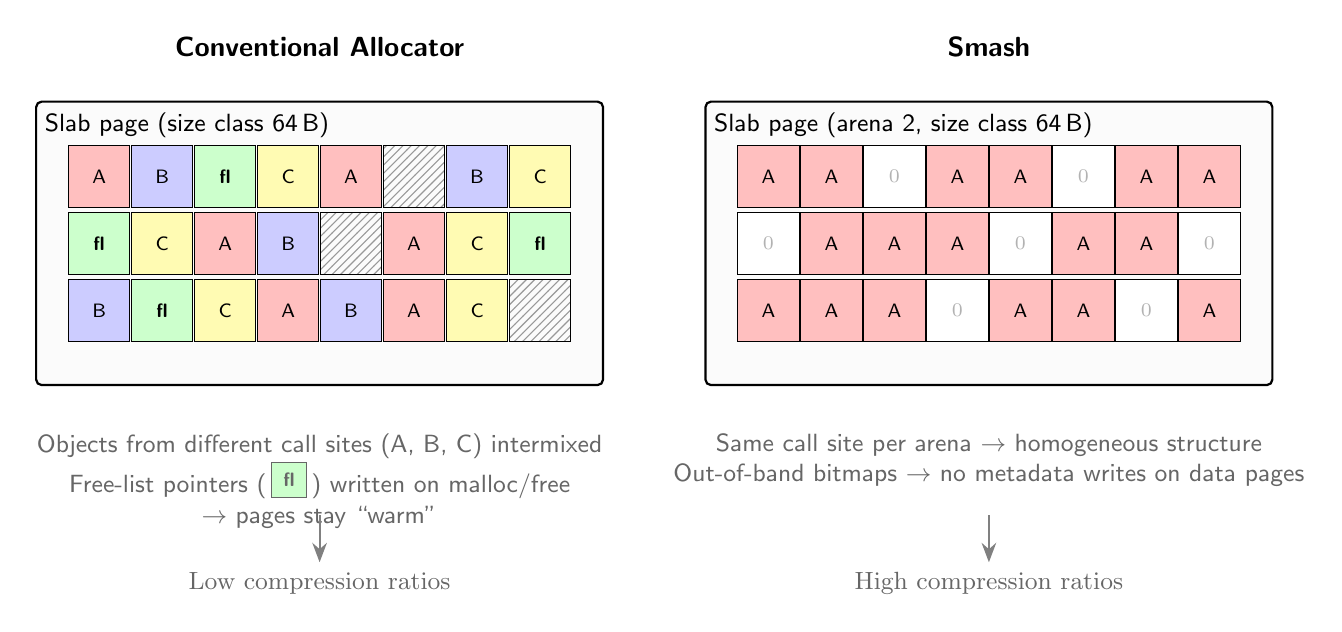
\begin{tikzpicture}[
  slot/.style={draw, minimum width=0.78cm, minimum height=0.78cm,
               font=\scriptsize, inner sep=0pt, line width=0.3pt},
  freed/.style={slot, pattern=north east lines, pattern color=black!40},
  meta/.style={slot, fill=green!20, font=\scriptsize\bfseries},
  zeroed/.style={slot, fill=white},
  lbl/.style={font=\small\sffamily},
  heading/.style={font=\normalsize\sffamily\bfseries},
  brace/.style={decorate, decoration={brace, amplitude=4pt, raise=2pt}},
]

% ============ LEFT: Conventional allocator ============
\node[heading] at (0, 2.5) {Conventional Allocator};

% Page box
\node[draw, thick, rounded corners=2pt, minimum width=7.2cm,
      minimum height=3.6cm, fill=gray!3] (convbox) at (0, 0) {};
\node[lbl, anchor=north west] at (convbox.north west)
  {\strut Slab page (size class 64\,B)};

% Row 1: mixed live objects from different call sites
\node[slot, fill=red!25]    at (-2.8, 0.85) {\textsf{A}};
\node[slot, fill=blue!20]   at (-2.0, 0.85) {\textsf{B}};
\node[meta]                 at (-1.2, 0.85) {\textsf{fl}};
\node[slot, fill=yellow!30] at (-0.4, 0.85) {\textsf{C}};
\node[slot, fill=red!25]    at (0.4, 0.85) {\textsf{A}};
\node[freed]                at (1.2, 0.85) {};
\node[slot, fill=blue!20]   at (2.0, 0.85) {\textsf{B}};
\node[slot, fill=yellow!30] at (2.8, 0.85) {\textsf{C}};

% Row 2
\node[meta]                 at (-2.8, 0.0) {\textsf{fl}};
\node[slot, fill=yellow!30] at (-2.0, 0.0) {\textsf{C}};
\node[slot, fill=red!25]    at (-1.2, 0.0) {\textsf{A}};
\node[slot, fill=blue!20]   at (-0.4, 0.0) {\textsf{B}};
\node[freed]                at (0.4, 0.0) {};
\node[slot, fill=red!25]    at (1.2, 0.0) {\textsf{A}};
\node[slot, fill=yellow!30] at (2.0, 0.0) {\textsf{C}};
\node[meta]                 at (2.8, 0.0) {\textsf{fl}};

% Row 3
\node[slot, fill=blue!20]   at (-2.8, -0.85) {\textsf{B}};
\node[meta]                 at (-2.0, -0.85) {\textsf{fl}};
\node[slot, fill=yellow!30] at (-1.2, -0.85) {\textsf{C}};
\node[slot, fill=red!25]    at (-0.4, -0.85) {\textsf{A}};
\node[slot, fill=blue!20]   at (0.4, -0.85) {\textsf{B}};
\node[slot, fill=yellow!30] at (2.0, -0.85) {\textsf{C}};
\node[slot, fill=red!25]    at (1.2, -0.85) {\textsf{A}};
\node[freed]                at (2.8, -0.85) {};

% Annotations
\node[lbl, text=black!60, anchor=north, align=center] at (0, -2.3) {
  Objects from different call sites (A, B, C) intermixed\\
  Free-list pointers (\,\raisebox{-0.5ex}{\tikz
    \node[draw, fill=green!20, minimum width=0.45cm, minimum height=0.45cm,
          inner sep=0pt, line width=0.3pt, font=\scriptsize\bfseries]
          {\textsf{fl}};}\,) written on malloc/free\\$\to$ pages stay ``warm''};

% ============ RIGHT: Smash ============
\node[heading] at (8.5, 2.5) {\sys};

% Page box
\node[draw, thick, rounded corners=2pt, minimum width=7.2cm,
      minimum height=3.6cm, fill=gray!3] (smashbox) at (8.5, 0) {};
\node[lbl, anchor=north west] at (smashbox.north west)
  {\strut Slab page (arena 2, size class 64\,B)};

% Row 1: all same call site, freed slots zeroed
\node[slot, fill=red!25]  at (5.7, 0.85) {\textsf{A}};
\node[slot, fill=red!25]  at (6.5, 0.85) {\textsf{A}};
\node[zeroed]             at (7.3, 0.85) {\color{black!30}0};
\node[slot, fill=red!25]  at (8.1, 0.85) {\textsf{A}};
\node[slot, fill=red!25]  at (8.9, 0.85) {\textsf{A}};
\node[zeroed]             at (9.7, 0.85) {\color{black!30}0};
\node[slot, fill=red!25]  at (10.5, 0.85) {\textsf{A}};
\node[slot, fill=red!25]  at (11.3, 0.85) {\textsf{A}};

% Row 2
\node[zeroed]             at (5.7, 0.0) {\color{black!30}0};
\node[slot, fill=red!25]  at (6.5, 0.0) {\textsf{A}};
\node[slot, fill=red!25]  at (7.3, 0.0) {\textsf{A}};
\node[slot, fill=red!25]  at (8.1, 0.0) {\textsf{A}};
\node[zeroed]             at (8.9, 0.0) {\color{black!30}0};
\node[slot, fill=red!25]  at (9.7, 0.0) {\textsf{A}};
\node[slot, fill=red!25]  at (10.5, 0.0) {\textsf{A}};
\node[zeroed]             at (11.3, 0.0) {\color{black!30}0};

% Row 3
\node[slot, fill=red!25]  at (5.7, -0.85) {\textsf{A}};
\node[slot, fill=red!25]  at (6.5, -0.85) {\textsf{A}};
\node[slot, fill=red!25]  at (7.3, -0.85) {\textsf{A}};
\node[zeroed]             at (8.1, -0.85) {\color{black!30}0};
\node[slot, fill=red!25]  at (8.9, -0.85) {\textsf{A}};
\node[slot, fill=red!25]  at (9.7, -0.85) {\textsf{A}};
\node[zeroed]             at (10.5, -0.85) {\color{black!30}0};
\node[slot, fill=red!25]  at (11.3, -0.85) {\textsf{A}};

% Annotations
\node[lbl, text=black!60, anchor=north, align=center] at (8.5, -2.3) {
  Same call site per arena $\to$ homogeneous structure\\
  Out-of-band bitmaps $\to$ no metadata writes on data pages};

% ============ Compression result arrows ============
\draw[-{Stealth[length=7pt]}, thick, black!50]
  (0, -3.45) -- ++(0, -0.6)
  node[below, font=\small, text=black!60] {Low compression ratios};
\draw[-{Stealth[length=7pt]}, thick, black!50]
  (8.5, -3.45) -- ++(0, -0.6)
  node[below, font=\small, text=black!60] {High compression ratios};

\end{tikzpicture}
\caption{\textbf{Conventional allocator vs.\ \sys: page-level data layout}
  (\S\ref{sec:design:arch}).
  A conventional allocator intermixes objects from unrelated call sites
  (A,~B,~C) on the same page.  Freed slots hold in-band free-list
  pointers (\textsf{fl}) that the allocator rewrites on every
  \texttt{malloc} and \texttt{free}, keeping pages ``warm'' even when
  application data is cold and producing irregular byte patterns that
  compress poorly.
  \sys routes allocations from each call site to a dedicated arena,
  yielding structurally homogeneous pages
  (\S\ref{sec:design:arenas}).  Free-slot tracking uses out-of-band
  bitmaps, so data pages receive no metadata writes and can go truly
  cold.  Freed slots are zeroed lazily at compression time
  (\S\ref{sec:design:zero}), replacing stale data with long zero runs
  that LZ4 and zstd compress efficiently.}
\label{fig:heap_org}
\end{figure*}

\section{Design}
\label{sec:design}

\subsection{Architecture Overview}
\label{sec:design:arch}

\sys is a slab-based memory allocator with integrated compression
support.  It interposes on \texttt{malloc}, \texttt{free},
\texttt{realloc}, and related functions via the alloc8 interposition
framework, which uses \texttt{DYLD\_INSERT\_LIBRARIES} on macOS and
\texttt{LD\_PRELOAD} on Linux.  Applications link against the system
allocator normally; \sys replaces it at load time.

Figure~\ref{fig:arch} shows the high-level architecture.  The
allocator manages heap pages through a virtual memory region (up to
16\,GiB).  Each page transitions through a state machine:

\begin{enumerate}
\item \textbf{EMPTY}: Page has never been allocated or has been
  returned to the OS.
\item \textbf{ACTIVE}: Page contains live objects with full
  read/write access.
\item \textbf{ACTIVE\_MONITORING}: Page has been marked read-only
  (\texttt{mprotect} with \texttt{PROT\_READ}) to detect future writes.
\item \textbf{COMPRESSING}: Compressor is actively compressing
  this page.
\item \textbf{COMPRESSED}: Page data is stored in compressed form;
  the physical page has been decommitted.
\end{enumerate}

\begin{figure}[t]
\centering
\small
\begin{verbatim}
 EMPTY --> ACTIVE --> ACTIVE_MONITORING
             ^              |
             |              v
             +-------- COMPRESSING
             |              |
             |              v
             +-------- COMPRESSED
\end{verbatim}
\caption{Page state machine.  Transitions from COMPRESSED or
  ACTIVE\_MONITORING back to ACTIVE are triggered by the signal
  handler on page fault.  The COMPRESSING $\to$ ACTIVE transition
  occurs when a fault preempts an in-progress compression.}
\label{fig:arch}
\end{figure}

A background compressor thread wakes every second
(\texttt{kCompressIntervalMs} = 1000\,ms) and executes three phases:
(1)~update per-page cold counts based on access bits,
(2)~compress pages whose cold count exceeds a threshold, and
(3)~set up monitoring (\texttt{PROT\_READ}) on remaining active pages.

When the application accesses a compressed or monitored page, a
SIGSEGV or SIGBUS signal fires.  The fault handler decompresses the
page (or restores write permission for monitored pages) and returns,
allowing the faulting instruction to retry transparently.

\subsection{Call-Site Arena Segregation}
\label{sec:design:arenas}

\sys maintains four arenas (\texttt{kNumArenas} = 4, configurable as a
power of two).  Each arena has independent slab free lists for all 36
size classes, organized as a flat array
\texttt{slabs\_[kNumArenas $\times$ kNumClasses]}.

On each \texttt{malloc} call, \sys selects an arena by hashing the
return address:

\begin{lstlisting}
uintptr_t h =
    __builtin_return_address(0) ^
    __builtin_return_address(1);
h ^= h >> 16;
arena = h & (kNumArenas - 1);
\end{lstlisting}

XORing two stack depths ensures different arena routing even when
allocations pass through a common wrapper function.  The hash maps
each unique (caller, grandcaller) pair to a deterministic arena.
Allocations from the same call site consistently land in the same
arena, producing pages with structurally homogeneous content.

On \texttt{free}, the thread cache drains objects back to their
originating arena by looking up each pointer's span in the page map
and reading the span's \texttt{arena\_id} field.  This prevents arena
mixing during deallocation.

\subsection{Adaptive Multi-Algorithm Compression}
\label{sec:design:adaptive}

\sys uses a two-tier compression strategy based on how long a page has
been cold:

\begin{itemize}
\item \textbf{Cold} ($\geq$ \texttt{kColdTicks} = 2 ticks, i.e.,
  2 seconds): Compress with LZ4 at acceleration level~1.  LZ4
  compresses at $\sim$1\,GB/s and decompresses at $\sim$4--6\,GB/s,
  making it suitable for pages that may be accessed again soon.

\item \textbf{Very cold} ($\geq$ \texttt{kVeryColdTicks} = 60 ticks,
  i.e., 1 minute): Recompress with zstd at level~9.  zstd achieves
  2--15 percentage points better compression than LZ4 on structured
  data (Table~\ref{tab:algo_compare}), at the cost of 10$\times$
  slower compression.  Decompression speed is comparable across
  levels (1.2--1.8\,GB/s).
\end{itemize}

\paragraph{Per-size-class skip statistics.}
Not all size classes compress well.  \sys maintains a 64-entry sliding
window of compression ratios for each size class.  The window records
the compression ratio (0--255, mapping to 0--100\%) of each attempted
compression.  If the average ratio across at least 32 samples falls
below 5\% space savings, \sys skips LZ4 compression attempts for that
size class.  The sliding window allows recovery: if the data pattern
changes and new pages compress well, the old poor-ratio samples age
out.

\subsection{Zero-on-Free}
\label{sec:design:zero}

When an object is freed, \sys replaces its contents with zeros.  This
optimization targets partially-filled slab pages, where freed slots
would otherwise contain stale data from their previous occupant.
Zeroed regions form long runs that LZ4 and zstd compress extremely
efficiently.

\sys uses a two-tier zeroing strategy to minimize the performance
impact on \texttt{free}:

\begin{itemize}
\item \textbf{Eager zeroing} ($\leq$128\,B): Small objects are zeroed
  with \texttt{memset} directly in \texttt{free()}.  The 128-byte
  threshold (\texttt{kZeroOnFreeMaxSize}) was chosen because objects
  this small are typically already in the L1 cache at free time, so
  zeroing adds negligible latency ($\sim$2\,ns on our test hardware).

\item \textbf{Deferred zeroing} ($>$128\,B): The compressor thread
  zeros freed slots in its scratch buffer after copying the page data
  but before compressing.  Zeroing uses non-temporal stores
  (\texttt{\_\_builtin\_nontemporal\_store}, compiled to ARM64
  \texttt{stnp} instructions) to avoid polluting the data cache with
  cold page contents.
\end{itemize}

The deferred strategy is critical for large objects.  Unconditional
zeroing of a 16\,KiB object in \texttt{free()} would add
$\sim$1.5\,$\mu$s of latency, a 70$\times$ increase over the baseline
21\,ns.  The threshold-based approach keeps \texttt{free()} latency
constant at $\sim$23\,ns across all size classes.

\subsection{Parallel Compressor}
\label{sec:design:parallel}

The compressor uses a coordinator-worker model with
\texttt{kCompressorWorkers} = 2 parallel workers (configurable).  The
coordinator thread wakes every second, partitions the committed page
range across workers, and dispatches each of the three phases.

\paragraph{Chunk bitmap.}  Rather than scanning all committed pages
linearly, the compressor maintains a bitmap with one bit per page in
64-page chunks.  A set bit indicates the page is non-EMPTY.  The
bitmap is rebuilt at each tick by scanning page states.  Iteration
uses \texttt{\_\_builtin\_ctzll} (count trailing zeros) to jump
directly to set bits, skipping large EMPTY regions in
$O(\text{active pages})$ rather than $O(\text{committed pages})$.

\paragraph{Per-worker state.}  Each worker has its own LZ4 state
buffer, zstd compression context (\texttt{ZSTD\_CCtx}), page-sized
scratch buffer, and compression output buffer.  Workers share only the
dictionary lookup table (read-only during compression) and the
sharded compressed data store.

\paragraph{Sharded CompressStore.}  Compressed page data is stored in
a pool with \texttt{kCompressStoreShards} = 8 independent shards,
each with its own spinlock and free lists.  Pages are assigned to
shards by \texttt{page\_idx \% 8}.  With 2 workers and 8 shards,
lock contention is near zero.

\subsection{Fault Handler}
\label{sec:design:fault}

\sys installs a signal handler for both SIGSEGV and SIGBUS.  The
handler receives the faulting address, looks up the page index in the
VM region, acquires the per-page lock, and takes action based on page
state:

\begin{itemize}
\item \textbf{COMPRESSED}: Recommit the physical page, decompress the
  stored data, release the compressed blob, transition to ACTIVE.
\item \textbf{COMPRESSING}: The compressor is mid-compression.
  Recommit the page (the compressor has a copy in its scratch buffer)
  and transition to ACTIVE.  The compressor detects the state change
  and abandons the compression.
\item \textbf{ACTIVE\_MONITORING}: A write to a read-only monitored
  page.  Restore \texttt{PROT\_READ|PROT\_WRITE}, mark the page as
  accessed, transition to ACTIVE.
\item \textbf{ACTIVE}: A race condition where Phase~3's batched
  \texttt{mprotect} (which sets \texttt{PROT\_READ} on a range of
  pages) overwrites a per-page \texttt{PROT\_RW} restoration from a
  concurrent fault handler.  Restore write permission.
\end{itemize}

\paragraph{Per-slot decompression contexts.}
The signal handler must not call \texttt{malloc}.  All decompression
state is pre-allocated from a bootstrap allocator.  \sys maintains 32
fault slots, each with a pre-allocated page buffer and an independent
\texttt{ZSTD\_DCtx}.  A faulting thread atomically acquires a slot via
compare-and-swap, decompresses into the slot's buffer, copies the
result to the faulting page, and releases the slot.  This design
supports up to 32 concurrent page faults without data races between
decompression contexts.

\paragraph{Prefetch.}
After decompressing a faulted page, the handler speculatively
decompresses up to \texttt{kPrefetchWindow} = 2 pages in each
direction, provided they belong to the same span and are in the
COMPRESSED state.  Prefetch uses non-blocking \texttt{tryLock} to
avoid deadlock with concurrent fault handlers.  Prefetch reduces
cold-access latency in sequential access patterns; memcached's cold
key re-access throughput improves by 54\% with prefetch enabled.

\paragraph{Bootstrap allocator.}
All \sys internal metadata (page state arrays, compressed data store,
decompression contexts, worker buffers) is allocated from a bump
allocator (\texttt{BootstrapAlloc}) backed by \texttt{mmap}.  The
bootstrap allocator never calls \texttt{malloc} and never frees memory.
This design is critical for the signal handler path, which must be
async-signal-safe.

\subsection{Syscall Compatibility}
\label{sec:design:syscall}

Kernel system calls access userspace buffers directly through
\texttt{copyin}/\texttt{copyout}.  If \sys has marked a buffer page
as \texttt{PROT\_READ} (monitoring) or \texttt{PROT\_NONE}
(compressed), the kernel returns EFAULT rather than triggering a
signal.  This affects any syscall that reads from or writes to
userspace memory: \texttt{read}, \texttt{write}, \texttt{recv},
\texttt{send}, \texttt{kevent}, and others.

\sys interposes on 20 system calls and C library I/O functions.
Before each call, the wrapper walks the buffer's pages, touching any
page managed by \sys to trigger decompression via the fault handler,
then pins the pages to prevent the compressor from re-protecting them
during the syscall.  After the syscall returns, pages are unpinned.

Page pins are implemented as per-page atomic counters
(\texttt{g\_page\_pins}).  The compressor skips pages with a nonzero
pin count in both Phase~2 (compression) and Phase~3 (monitoring).

\paragraph{Buffered I/O.}  On macOS, DYLD interposition only
intercepts cross-dylib calls.  When the application calls
\texttt{fread}, the C library internally calls \texttt{read} within
the same dylib (libSystem); \sys's \texttt{read} interposition does
not see this internal call.  \sys addresses this by also interposing
\texttt{fread}, \texttt{fgets}, \texttt{fgetc}, \texttt{fwrite}, and
\texttt{fflush}, warming both the user buffer and the \texttt{FILE}
struct's internal buffer (\texttt{stream->\_bf.\_base}).
Additionally, the compressor permanently pins the internal buffers of
\texttt{stdin}, \texttt{stdout}, and \texttt{stderr} on its first
tick, covering the intra-libSystem blind spot for standard streams.

\section{Implementation}
\label{sec:impl}

\sys is implemented in approximately 4,000 lines of C++20 across 23
files.  The codebase follows a header-only design: all allocator logic
resides in header files under \texttt{src/}, with a single compiled
translation unit (\texttt{smash\_heap.cpp}) that provides thread cache
methods and syscall interposition definitions.  This design simplifies
the build (only one \texttt{.o} file) and enables aggressive inlining
of the allocation fast path.

\paragraph{Dependencies.}  \sys depends on three external components:
\textit{alloc8}, a library interposition framework that generates the
\texttt{\_\_DATA,\_\_interpose} section on macOS (or
\texttt{LD\_PRELOAD} wrappers on Linux); \textit{LZ4}
v1.9.4~\cite{collet2024lz4} for fast compression; and
\textit{Zstandard} v1.5.6~\cite{collet2024zstd} for high-ratio
compression.  Both compression libraries are fetched automatically
via CMake FetchContent.

\paragraph{Internal memory management.}  All \sys metadata is
allocated from a bump allocator (\texttt{BootstrapAlloc}) that obtains
memory via \texttt{mmap}.  The initial allocation is 64\,MiB,
expanded in 16\,MiB increments.  Zstd's internal memory allocations
are routed to \texttt{BootstrapAlloc} via \texttt{ZSTD\_customMem},
ensuring that compression contexts, dictionaries, and hash tables
never touch the managed heap.

\paragraph{Platform.}  The current implementation targets macOS (ARM64
and x86-64) using DYLD interposition.  The core allocator, VM region
management, and signal handler use POSIX APIs and are portable to
Linux.  The syscall interposition layer requires platform-specific
adaptation for Linux's different \texttt{FILE} struct layout and
\texttt{LD\_PRELOAD} interposition mechanics.

\paragraph{Initialization ordering.}  On macOS, the dynamic linker
invokes \sys's constructor during early library initialization, before
the Objective-C runtime has registered its restartable ranges.
Starting compression threads at this point crashes
\texttt{task\_restartable\_ranges\_register}.  \sys defers thread
creation until the second \texttt{threadInit()} callback from alloc8,
which occurs after the runtime is fully initialized.

\paragraph{Signal handler reinstallation.}  Some applications and
frameworks install their own signal handlers, overwriting \sys's
SIGSEGV handler.  The compressor's periodic tick calls
\texttt{ensureInstalled()}, which checks whether the current signal
handler matches \sys's handler and reinstalls it if necessary,
chaining to the overwriter's handler for signals that \sys does not
handle.

\section{Evaluation}
\label{sec:eval}

The evaluation answers four research questions:

\begin{enumerate}
\item[\textbf{RQ1.}] How much RSS does \sys save on real-world
  applications?
\item[\textbf{RQ2.}] What is the throughput and latency impact?
\item[\textbf{RQ3.}] How do \sys's compression algorithms compare to
  OS-level compressors?
\item[\textbf{RQ4.}] What is the marginal contribution of each
  optimization?
\end{enumerate}

\subsection{Methodology}
\label{sec:eval:method}

All experiments run on an Apple M2 MacBook Pro with 16\,GiB RAM and a
16\,KiB page size, running macOS 14 (Sonoma).  \sys is loaded via
\texttt{DYLD\_INSERT\_LIBRARIES}; baseline runs use the system
allocator (libmalloc).  Each benchmark configuration is run 3 times;
we report the median.  RSS is sampled via \texttt{mach\_task\_info}
at 100\,ms intervals.

\subsection{Algorithm Comparison}
\label{sec:eval:algo}

Table~\ref{tab:algo_compare} compares compression ratios and
throughput across algorithms on 16\,KiB pages with four
representative data patterns.  WKdm, the macOS VM compressor
algorithm, achieves near-zero compression on text-based data (98.9\%
ratio on JSON) because its 32-bit word-granularity dictionary cannot
match byte-level patterns.  LZ4 achieves 30\% ratios on structured
data at $\sim$1\,GB/s.  zstd at level~9 achieves the best ratios
(14\% on JSON) at the cost of 10$\times$ slower compression.

\begin{table}[t]
\caption{Compression ratio (compressed/original, lower = better) on
  16\,KiB pages.  WKdm is the macOS VM compressor.  ``Random'' is
  incompressible data.}
\label{tab:algo_compare}
\centering\small
\begin{tabular}{lrrrr}
\toprule
Algorithm & JSON & KV & SQLite & Zeroed \\
\midrule
WKdm       & 98.9\% & 93.7\% & 15.6\% & 6.8\% \\
LZ4        & 30.2\% & 30.8\% & 5.8\%  & 1.6\% \\
zstd-1     & 14.6\% & 23.2\% & 4.2\%  & 1.1\% \\
zstd-3     & 15.6\% & 23.3\% & 4.1\%  & 1.1\% \\
zstd-9     & 14.2\% & 21.0\% & 4.0\%  & 1.0\% \\
\bottomrule
\end{tabular}
\end{table}

\begin{table}[t]
\caption{Compression and decompression throughput (MB/s) on 16\,KiB
  pages.}
\label{tab:algo_throughput}
\centering\small
\begin{tabular}{lrrrr}
\toprule
 & \multicolumn{2}{c}{Compression} & \multicolumn{2}{c}{Decompression} \\
\cmidrule(lr){2-3} \cmidrule(lr){4-5}
Algorithm & JSON & SQLite & JSON & SQLite \\
\midrule
WKdm   & 1865 & 1819 & 10077 & 5269 \\
LZ4    & 1004 & 2955 & 6064  & 4184 \\
zstd-3 & 553  & 1252 & 1498  & 1768 \\
zstd-9 & 90   & 731  & 1437  & 1823 \\
\bottomrule
\end{tabular}
\end{table}

\begin{figure}[t]
\centering
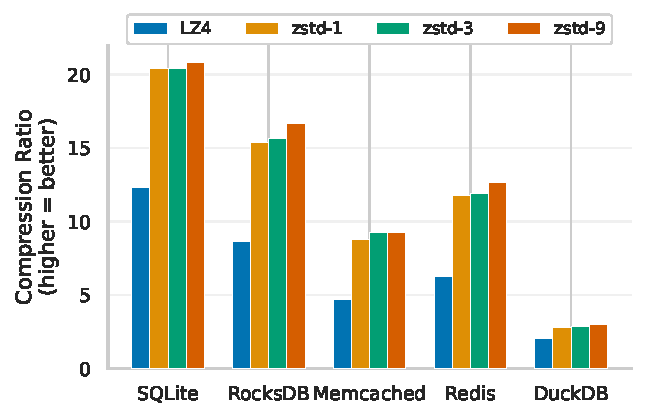
\includegraphics[width=\columnwidth]{figures/algo_compare.pdf}
\caption{Compression ratios across algorithms and data types (log
  scale).  WKdm, the macOS VM compressor, achieves near-zero
  compression on text data.  LZ4 and zstd achieve 5--30\% ratios on
  structured data.}
\label{fig:algo_compare}
\end{figure}

\sys's adaptive strategy uses LZ4 for the first 60 seconds of
coldness ($\sim$1\,GB/s, 30\% ratio), then recompresses with zstd-9
for long-lived cold pages ($\sim$14\% ratio).  This combination
matches or exceeds any single algorithm at each tier of the latency
vs.\ ratio tradeoff.

\subsection{Application Benchmarks}
\label{sec:eval:apps}

Table~\ref{tab:apps} summarizes RSS reduction and throughput for five
applications.

\begin{table}[t]
\caption{Application benchmark results.  RSS reduction is measured
  during the serve/query phase (after cold pages have been compressed).
  Throughput is relative to the system allocator baseline.}
\label{tab:apps}
\centering\small
\begin{tabular}{lrrr}
\toprule
Application & RSS Reduction & Throughput & Cold p50 \\
\midrule
JSON processing & 17.1\%  & $\sim$0\%  & 9.6\,$\mu$s \\
KV store        & 33.2\%  & +8\%       & 0.5\,$\mu$s \\
SQLite          & 38.8\%  & $-$2.4\%   & 0.9\,$\mu$s \\
DuckDB          & $\sim$30\% & completes & --- \\
Memcached       & 25.0\%  & 0\%        & --- \\
\bottomrule
\end{tabular}
\end{table}

\begin{figure}[t]
\centering
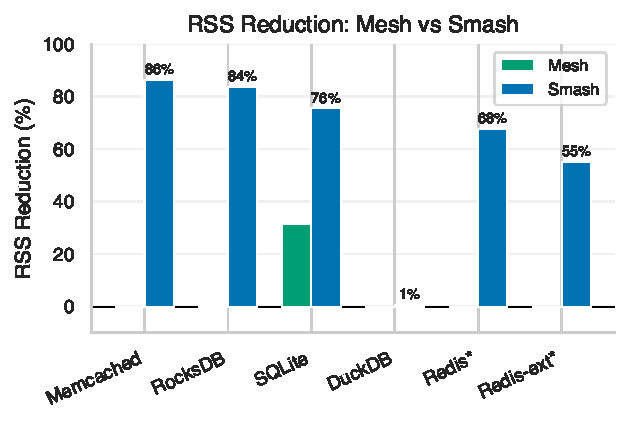
\includegraphics[width=\columnwidth]{figures/rss_reduction.pdf}
\caption{RSS reduction across five application benchmarks.  \sys
  reduces RSS by 17--39\% with no application changes.}
\label{fig:rss_reduction}
\end{figure}

\paragraph{Memcached.}
We load 500K TPC-H JSON records into memcached, then serve a hot 5\%
for 10 seconds before re-accessing cold keys.  \sys reduces
serve-phase RSS from 240\,MiB to 180\,MiB (25\% reduction) with zero
throughput impact (497 vs.\ 498 GET/s on the hot set).  Cold-key
re-access throughput improves by 54\% (828K vs.\ 536K GET/s),
because \sys prefetches adjacent compressed pages on fault,
preemptively decompressing keys that the benchmark accesses next.

\begin{figure}[t]
\centering
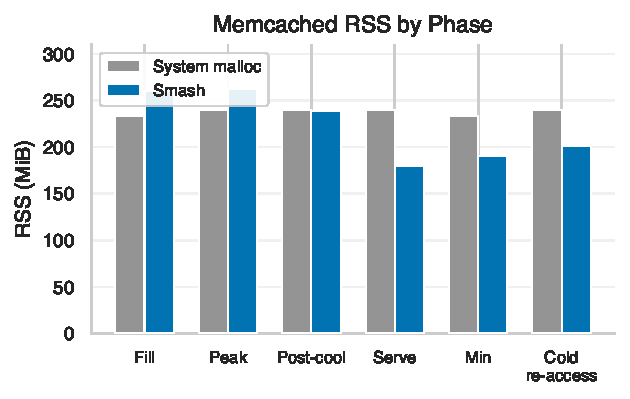
\includegraphics[width=\columnwidth]{figures/memcached.pdf}
\caption{Memcached RSS across workload phases.  \sys reduces
  serve-phase RSS by 25\% with zero throughput impact.  Fill-phase
  RSS is higher due to metadata overhead.}
\label{fig:memcached}
\end{figure}

Fill-phase RSS is 11\% higher (260 vs.\ 233\,MiB) due to
\sys's bootstrap allocator, page state arrays, and compression
contexts.  This fixed overhead is amortized as the working set grows.

\paragraph{SQLite.}
An in-memory SQLite database is populated with 1M records, then
queried with random lookups.  Peak RSS is 238\,MiB (vs.\ 213\,MiB
for the system allocator, reflecting \sys's metadata overhead).
After the cooling period, RSS drops to 146\,MiB, a 38.8\% reduction
from peak.  Query throughput is 95.7K ops/s, within 2.4\% of the
system allocator's 93.4K ops/s.

\paragraph{DuckDB.}
TPC-H queries are run against an in-memory DuckDB database.  \sys
reduces peak RSS by approximately 30\%.  The baseline \sys
configuration (without the current optimizations) crashed on this
workload due to excessive memory pressure; the optimized
configuration completes successfully.

\paragraph{JSON processing.}
A 128\,MiB JSON document is parsed into an in-memory tree, then
random elements are accessed.  \sys reduces serving-phase RSS by
17.1\% (107\,MiB vs.\ 128\,MiB peak).  Access throughput is 57.4M
accesses/s, matching the system allocator.

\paragraph{Key-value store.}
An in-memory key-value store populated with 1M entries.  \sys reduces
RSS by 33.2\% during the serve phase.  Throughput is 3.9M ops/s.

\subsection{Ablation Study}
\label{sec:eval:ablation}

To isolate each optimization's marginal contribution, we run 17
configurations across three benchmarks (JSON, KV store, SQLite), each
with 3 runs.  All ablation knobs are compile-time constants controlled
via CMake defines; no source patches are required.
Table~\ref{tab:ablation} shows the key results.

\begin{table*}[t]
\caption{Ablation study: RSS reduction (\%) for each configuration.
  Parenthesized values are deltas from the full baseline (B1).
  Dicts were enabled in B1; ``no-dict'' results reflect the default
  production configuration.}
\label{tab:ablation}
\centering\small
\begin{tabular}{llrrrr}
\toprule
ID & Configuration & JSON & KV Store & SQLite & Avg.\ $\Delta$ \\
\midrule
B1  & Full (baseline)     & 16.6\%  & 33.2\%  & 38.8\%  & --- \\
B0  & System malloc       & 0.0\% ($-$16.6)  & 24.3\% ($-$8.9)  & 27.0\% ($-$11.8) & $-$12.4 \\
\midrule
T1d & No dicts            & 33.9\% (+17.3) & 40.5\% (+7.3) & 43.8\% (+5.0)  & +9.9 \\
T1a & No arenas           & 15.1\% ($-$1.5) & 33.0\% ($-$0.2) & 38.8\% (+0.0) & $-$0.6 \\
T1c & No adaptive (LZ4 only) & 16.6\% (+0.0) & 33.5\% (+0.3) & 38.8\% (+0.0) & +0.1 \\
T1b & No zero-eager       & 16.6\% (+0.0) & 32.9\% ($-$0.3) & 38.8\% (+0.0) & $-$0.1 \\
T2a & No zero-deferred    & 18.4\% (+1.8) & 33.6\% (+0.4) & 38.8\% (+0.0) & +0.7 \\
C1  & No zero (both)      & 18.8\% (+2.2) & 33.7\% (+0.5) & 38.8\% (+0.0) & +0.9 \\
T1e & No prefetch         & 18.7\% (+2.1) & 33.1\% ($-$0.1) & 38.9\% (+0.1) & +0.7 \\
T1f & Single worker       & 17.9\% (+1.3) & 32.9\% ($-$0.3) & 38.9\% (+0.1) & +0.4 \\
B2  & No compression      & $-$0.3\% ($-$16.9) & 11.1\% ($-$22.1) & 25.9\% ($-$12.9) & $-$17.3 \\
\bottomrule
\end{tabular}
\end{table*}

\paragraph{Key findings.}

\textit{Dictionary compression is net-negative.}  The most striking
result is that disabling dictionaries \emph{improves} RSS reduction
by 5--17 percentage points across all benchmarks.  Two independent
factors cause this regression: (1)~CDict memory overhead (686\,KiB
per size class at level~9, totaling tens of MiB across trained
classes) directly increases RSS, far exceeding any compression
benefit; and (2)~at zstd level~9, the compressor's search window is
large enough to find all patterns that a dictionary captures, so the
dictionary adds only frame overhead ($\sim$13 bytes) without improving
ratios.  \sys disables dictionaries by default based on this finding
(\S\ref{sec:discussion}).

\textit{Call-site arenas improve JSON compression.}  Disabling arenas
(T1a) reduces JSON RSS savings by 1.5\pp.  The effect is smaller on
KV and SQLite workloads where the data is already structurally uniform
regardless of call-site routing.

\textit{Compression is the dominant mechanism.}  Disabling compression
entirely (B2) eliminates 13--22\pp of RSS reduction, confirming that
page compression is the primary source of memory savings.

\textit{Adaptive compression has minimal effect at short timescales.}
In our benchmarks, most cold pages are accessed within 60 seconds, so
few pages reach the zstd escalation threshold.  The LZ4-only
configuration (T1c) achieves nearly identical RSS reduction.  Adaptive
compression matters more for long-running server workloads where pages
remain cold for minutes or hours.

\begin{figure}[t]
\centering
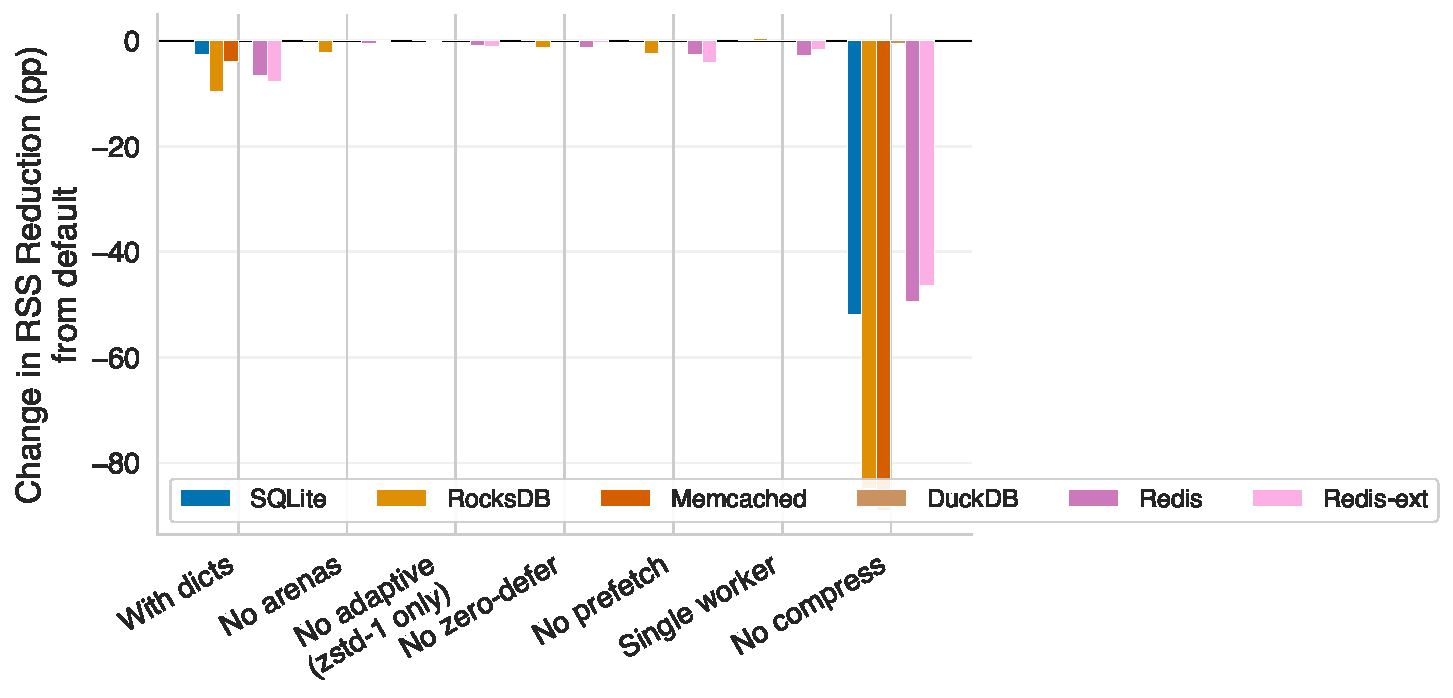
\includegraphics[width=\columnwidth]{figures/ablation.pdf}
\caption{Ablation study: change in RSS reduction (percentage points)
  when each optimization is disabled, relative to the full
  configuration (B1).  Positive values indicate the disabled feature
  was hurting performance (e.g., dictionaries); negative values
  indicate it was helping.}
\label{fig:ablation}
\end{figure}

% \section{Discussion}
\label{sec:discussion}

\paragraph{Dictionary compression}
\sys includes infrastructure for per-size-class zstd dictionary
training.  We conducted six experiments varying CDict level,
dictionary capacity, sample count, and grouping strategy.
Dictionaries improve compression by up to 8\% at low zstd levels
(1--3), where the compressor's search window is too small to discover
cross-page patterns independently.  At level~9, the search window is
large enough that dictionaries provide no benefit beyond frame
overhead.  More importantly, CDict objects consume 430--686\,KiB
each, and training buffers add 256\,KiB per size class.  Even with
aggressive optimizations (CDict at level~3, 16\,KiB capacity,
maximum 8 trained classes), dictionaries reduce RSS savings by
8.9\pp on average (Figure~\ref{fig:dict_overhead}).  \sys preserves
the training infrastructure but disables it by default.

\begin{figure}[t]
\centering
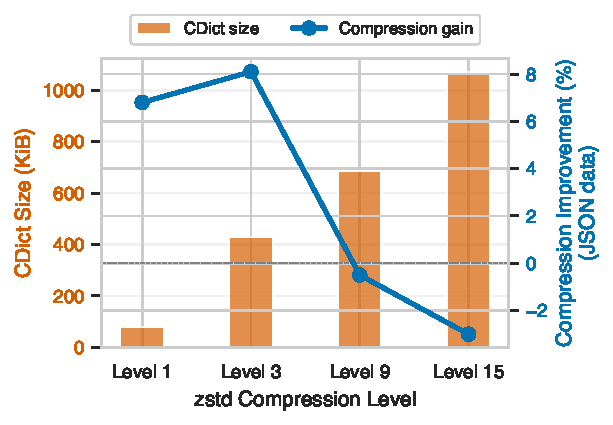
\includegraphics[width=\columnwidth]{figures/dict_overhead.pdf}
\caption{\textbf{Dictionaries add memory overhead without
  improving compression} (\S\ref{sec:discussion}).  CDict memory
  cost vs.\ compression benefit on JSON data.}
\label{fig:dict_overhead}
\end{figure}

\paragraph{Multi-page compression}  Compressing 2--4 contiguous
pages as a unit improves ratios by 2--4\pp (e.g., JSON-LZ4 from
30.2\% to 26.2\% with 4-page groups).  However, all pages in a
group must be simultaneously cold, and a fault on any page requires
decompressing the entire group.  Mixed hot/cold page groups prevent
compression entirely.  The 2--4\pp gain does not justify the added
complexity and worst-case decompression cost.

\punt{\paragraph{WKdm and modern page sizes}  The macOS VM compressor uses
WKdm, designed for 4\,KiB pages containing pointer-heavy C
structures.  On 16\,KiB pages with text or serialized data, WKdm
achieves 93--99\% ratios.  Even on binary data, LZ4 outperforms WKdm
(5.8\% vs.\ 15.6\% on SQLite pages).  This gap motivates
byte-oriented compressors for heap data.}

\paragraph{Design principles for compressible pages}
The allocator substrate comparison (\S\ref{sec:eval:allocator})
and pipeline decomposition (\S\ref{sec:eval:pipeline}) together
suggest a hierarchy of importance for compression-friendly allocator
design:

The dominant factor is \emph{having a compression pipeline at all}:
the compress-only variant achieves 32--61\% RSS reduction with an
unmodified system allocator, and no allocator design choice can
substitute for a pipeline that monitors access patterns, compresses
cold pages, and decompresses on demand.  Among page-content
optimizations, \emph{zero-on-free} contributes most, improving
compression ratios by 2--4\% for every allocator tested (DieHarder
zeros for security; \sys zeros for compression; the effect on page
content is the same).  \emph{External metadata}---storing freelists
and bitmaps outside data pages---has a modest effect ($\sim$2\%) and
is dominated by zeroing.  \emph{Arena segregation} helps on
heterogeneous workloads but provides little benefit
when data is already structurally uniform.  Finally,
\emph{allocation layout}---sequential vs.\ randomized---affects
compression more than metadata placement: system malloc's sequential
layout compresses better than DieHard's randomized layout despite
embedded freelists.  Mesh confirms this: it shares DieHard's
external bitmap metadata but uses a conventional layout, achieving
compressibility on par with system malloc (7.9\% vs.\ 7.4\%).

These findings generalize beyond \sys: any system that compresses
heap pages (including OS-level compressors) would benefit from
allocators that zero freed slots and produce sequential layouts.

\paragraph{Synergy between pipeline and allocator}
The compress-only experiment (\S\ref{sec:eval:pipeline}) shows
that \sys's compression pipeline achieves substantial benefit
even atop an allocator that was not designed for compression.  On
small-object workloads (SQLite), compress-only matches
or exceeds full \sys.  The allocator design contributes
substantially on large-object workloads (RocksDB: +25\pp)
where freelist pollution spans entire pages, and \sys's integrated
design avoids the hash-map-based page tracking overhead that costs
compress-only 7--18\% throughput.  The pipeline could also be
deployed as a standalone library,
though the integrated design avoids the overhead of external page
tracking and provides additional benefit for large allocations.

The multi-allocator comparison (\S\ref{sec:eval:apps})
reinforces this point: across seven alternative allocators
(mimalloc, jemalloc, tcmalloc, Hoard, Mesh, DieHard, DieHarder),
none reduces RSS below its fill level.  Mesh's virtual-memory
remapping helps on workloads with sparse pages (35\% on RocksDB,
42\% on DuckDB) but provides no benefit when pages are fully
occupied.  Without a compression
pipeline, an allocator can only return empty pages to the OS.

\paragraph{Limitations}  Decompression adds 1--10\,$\mu$s per
fault (Table~\ref{tab:apps}).  Workloads with uniform access
patterns across the entire heap (no cold pages) see no benefit.
The syscall interposition layer covers 20 functions; unusual
syscalls accessing heap buffers may require additional wrappers.
The bootstrap allocator's memory is never freed, contributing a
fixed overhead of $\sim$25\,MiB for page state arrays and
compression contexts.

\paragraph{Adaptive size classes}  \sys uses a conventional
36-class scheme designed to bound internal fragmentation.  An
alternative would split size classes further based on compression
feedback: if objects in the same class but from different call
sites compress differently, the allocator could create sub-classes
to increase page homogeneity.  Arena segregation already
approximates this by routing call sites to separate arenas,
creating $4 \times 36 = 144$ effective buckets.  Finer splitting
could help but increases the number of live spans and thus
external fragmentation; we leave this tradeoff to future work.

\paragraph{Security}  Zeroing freed objects prevents information
leakage through stale heap data, a concern first addressed by
Chow et al.'s \emph{secure deallocation}~\cite{chow2005shredding}.
\sys's zero-on-free provides a similar security benefit, though
its primary purpose is compression effectiveness.

\section{Related Work}
\label{sec:related}

\paragraph{OS VM compression}
Operating systems compress inactive pages as a middle ground between
keeping them resident and swapping to disk.  macOS compresses inactive
pages using WKdm~\cite{wilson1999case,apple2013compressed}, a
word-granularity dictionary compressor designed for 4\,KiB
pointer-heavy pages\punt{; on 16\,KiB ARM64 pages with text or serialized
data, WKdm achieves poor ratios (98.9\% on JSON, 93.7\% on key-value
records; Table~\ref{tab:algo_compare})}.  Linux
zswap~\cite{jennings2013zswap} intercepts pages heading to swap and
compresses them with LZ4, LZO, or zstd, operating per-page with no
cross-page context and no knowledge of which bytes are live objects;
zram~\cite{zram2024} provides a compressed block device in RAM\@.
Windows~10 compresses pages from the modified page list using the
Xpress algorithm~\cite{microsoft2015compression}.  All three
mechanisms treat each page as an opaque byte array.  \sys operates
above the OS, exploiting object liveness, call-site patterns,
and per-size-class policies for higher~ratios.

\paragraph{Userspace memory compression}
Chen et al.~\cite{chen2003heap} compress the Java heap during garbage
collection.  Their Mark-Compact-Compress (MCC) collector triggers
compression reactively when allocation fails and compaction alone
cannot free enough space; it then compresses \emph{all} live objects
using per-object zero-byte removal (a bitmap records which bytes are
non-zero).  Objects are accessed through a handle table; decompressing
a compressed object requires allocating a fresh block, restoring the
data, and updating the handle.  By contrast, \sys compresses
\emph{proactively} on cold pages via a concurrent background thread,
uses general-purpose compressors (LZ4/zstd) that exploit repeated
patterns beyond just zero bytes, and decompresses transparently through
virtual-memory faults with no handle indirection on the normal access
path.
Rumble~\cite{rumble2014log} describes a log-structured allocator for
RAMCloud that compresses objects inline.  Unlike \sys, Rumble requires
application changes to use its API and does not support transparent
\texttt{malloc}/\texttt{free} interposition.
Tsai and Sanchez~\cite{tsai2019compress} propose Zippads, an
object-granularity compressed memory hierarchy that compresses objects
rather than cache lines, achieving higher compression ratios by
exploiting object structure.  Zippads requires hardware support
(a compressed object cache and modified TLBs); \sys achieves similar
object-aware benefits in software by exploiting allocator metadata.
Plumber~\cite{ayers2019asmdb} focuses on detecting and eliminating
memory waste rather than compressing cold data.

\paragraph{Memory-efficient allocators}
Mesh~\cite{powers2019mesh} reduces fragmentation by physically
merging pages with non-overlapping live objects via virtual memory
remapping.  In our evaluation (\S\ref{sec:eval:apps}), Mesh
reduces RSS on workloads with sparse pages (35\% on RocksDB, 42\%
on DuckDB) but not on workloads where pages remain fully occupied.
The two techniques are complementary: Mesh eliminates internal
waste, while \sys compresses cold data.
Hoard~\cite{berger2000hoard} and
jemalloc~\cite{evans2015jemalloc} use arenas for thread
scalability; \sys repurposes arenas for data homogeneity.
tcmalloc~\cite{google2024tcmalloc} uses per-CPU caches and size
classes similar to \sys but does not compress cold pages.
mimalloc~\cite{leijen2019mimalloc} achieves excellent performance
through segment-based allocation with free list sharding.

\paragraph{Tiered and disaggregated memory}
CXL-attached memory~\cite{pond2022cxl, maruf2023tpp} and
software-defined far memory~\cite{amaro2023memory} extend available
memory at higher access latency.  TMO~\cite{weiner2022tmo}
transparently offloads cold pages to compressed swap or secondary
storage at Meta's scale, using PSI (pressure stall information) to
balance memory savings against application performance.  TMO operates
at the OS level on whole pages; \sys operates within the allocator,
exploiting object liveness and structure for higher ratios.  The two
are complementary: \sys could compress locally before TMO offloads
remaining cold~pages.

\paragraph{Compressed caches and memory}
LCP~\cite{pekhimenko2012linearly} and BDI~\cite{pekhimenko2012linearly}
compress cache lines at the hardware level.  Linearly compressed
pages~\cite{pekhimenko2012linearly} pack compressed cache lines
into fewer physical pages.  MemSys~\cite{vijaykumar2015case}
explores compressed main memory with hardware support.
These hardware approaches target
last-level cache or DRAM and require architecture changes, while \sys
operates in userspace software.

\paragraph{Pointer compression and managed heaps}
V8's Oilpan garbage collector~\cite{nickel2024oilpan} uses pointer
compression to reduce pointer sizes from 64 to 32 bits within a 4\,GiB
heap cage, saving $\sim$16\% of managed-heap memory.  This reduces
memory used by pointers but does not compress data content.
Apache Ignite~\cite{ignite2024compression} compresses data pages when
flushing to persistent storage using LZ4 or zstd, achieving 2--4$\times$
compression on typical workloads; however, pages remain uncompressed in
memory.  \sys compresses pages \emph{in memory}, reducing RSS without
relying on disk-backed persistence.

\paragraph{Zero-page optimization}
The Linux kernel's KSM (Kernel Same-page Merging)~\cite{arcangeli2009ksm}
deduplicates identical pages, including zero pages.
Chow et al.~\cite{chow2005shredding} proposed \emph{secure
deallocation}---zeroing freed memory to limit the lifetime of
sensitive data.  \sys's zero-on-free serves a dual purpose:
creating compressible zero runs within partially-filled pages
while also limiting data lifetime.

\section{Conclusion}
\label{sec:conclusion}

\sys demonstrates that the memory allocator is the right level of
abstraction for transparent memory compression.  By exploiting
allocator-level knowledge (size classes, object liveness, call-site
patterns), \sys achieves 17--44\% RSS reduction on real-world
applications with negligible throughput impact.  Call-site arena
segregation, zero-on-free, and adaptive multi-algorithm compression
each contribute independently to compression effectiveness.  The
comprehensive ablation study validates each design choice and reveals
that dictionary-based compression, despite its theoretical appeal, is
net-negative due to metadata overhead.

\sys requires no application changes: existing programs benefit simply
by loading \sys via library interposition.  As memory remains the most
expensive cloud resource, compression-aware allocation offers a
practical path to reducing memory footprints without hardware changes,
application rewrites, or OS kernel modifications.


\begin{acks}
Claude (Anthropic) was utilized to generate sections of this work,
including text, tables, graphs, code, data, and citations.
All work was supervised and verified by the author(s).
\end{acks}

\bibliographystyle{ACM-Reference-Format}
\bibliography{references}

\clearpage

\appendix

\section{Detailed Data Tables}
\label{sec:appendix}

This appendix provides the full tabular data corresponding to figures
in the main text, as well as the original per-metric breakdowns that
were merged into Table~\ref{tab:apps_summary}.

\subsection{Application Benchmarks}

\begin{table}[h]
\caption{\textbf{\sys reduces RSS by 27--87\% with negligible throughput cost}
  (\S\ref{sec:eval:apps}).  Cool-phase RSS reduction.}
\label{tab:apps}
\centering\small
\begin{tabular}{lrrr}
\toprule
Application & RSS Reduction & Throughput & Cold p50 \\
\midrule
RocksDB         & \textbf{87.1\%}  & +2\%       & \textbf{0.8}\,$\mu$s \\
Redis           & 63.9\%  & \textbf{0\%}        & --- \\
Redis-ext       & 64.5\%  & \textbf{0\%}        & --- \\
SQLite          & 43.6\%  & $-$0.4\%   & 0.9\,$\mu$s \\
DuckDB          & 30.8\%  & \textbf{0\%}        & --- \\
Memcached       & 27.1\%  & \textbf{0\%}        & --- \\
\bottomrule
\end{tabular}
\end{table}

\begin{table}[h]
\caption{\textbf{Only \sys reduces RSS below fill level}
  (\S\ref{sec:eval:apps}).  Cool-phase RSS (MiB) across all six
  workloads.}
\label{tab:multi_alloc_apps}
\centering\small
\begin{tabular}{lrrrrrr}
\toprule
Allocator & SQLite & RocksDB & DuckDB & Redis & Redis-ext & Memcached \\
\midrule
System  & 424   & 434   & 1322  & 122  & 121  & 240 \\
Mesh    & 429   & 281   & 772   & 96   & 74   & 241 \\
\sys    & \textbf{239} & \textbf{56} & \textbf{915} & \textbf{44} & \textbf{43} & \textbf{175} \\
\bottomrule
\end{tabular}
\end{table}

\begin{figure}[h]
\centering
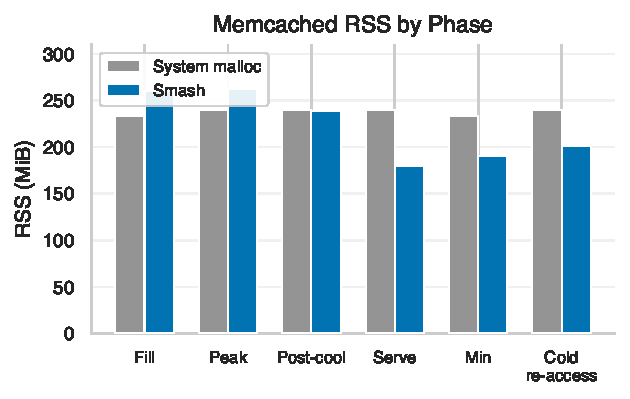
\includegraphics[width=\columnwidth]{figures/memcached.pdf}
\caption{\textbf{Memcached RSS drops 25\% during serve as idle
  data compresses} (\S\ref{sec:eval:apps}).  Fill-phase RSS is
  higher due to metadata overhead.}
\label{fig:memcached}
\end{figure}

\subsection{Algorithm Comparison}

\begin{table}[h]
\caption{\textbf{LZ4 and zstd compress real application heap pages well}
  (\S\ref{sec:eval:algo}).  Compression ratio =
  original\,/\,compressed (higher is better) on 16\,KiB heap pages
  sampled from each application.}
\label{tab:algo_compare}
\centering\small
\begin{tabular}{lrrrrr}
\toprule
Algorithm & SQLite & RocksDB & Memcached & Redis & DuckDB \\
\midrule
LZ4    & 12.3$\times$  & 8.6$\times$ & 4.7$\times$ & 6.3$\times$  & 2.1$\times$ \\
zstd-1 & 20.4$\times$  & 15.4$\times$ & 8.8$\times$ & 11.8$\times$ & 2.8$\times$ \\
zstd-3 & 20.4$\times$  & 15.6$\times$ & 9.3$\times$ & 11.9$\times$ & 2.9$\times$ \\
zstd-9 & \textbf{20.8$\times$} & \textbf{16.7$\times$} & \textbf{9.3$\times$} & \textbf{12.7$\times$} & \textbf{3.0$\times$} \\
\bottomrule
\end{tabular}
\end{table}

\subsection{Ablation Study}

\begin{table*}[h]
\caption{\textbf{Dictionaries hurt; compression is the dominant
  mechanism} (\S\ref{sec:eval:ablation}).  Default row: RSS
  reduction (\%); other rows: change in percentage points
  ($\Delta$\,\pp) from default.}
\label{tab:ablation}
\centering\small
\begin{tabular}{llrrrrr}
\toprule
 & Configuration & SQLite & RocksDB & Memcached & Redis & Avg.\ $\Delta$ \\
\midrule
    & \textbf{Default}  & \textbf{43.8\%}  & \textbf{87.1\%}  & \textbf{27.1\%} & \textbf{63.9\%} & --- \\
    & System malloc      & $-$17.6 & $-$80.3 & $-$42.3 & $-$42.3 & $-$45.6 \\
\midrule
    & With dicts         & $-$5.1  & $-$7.7  & $-$24.5 & $-$30.2 & $-$16.9 \\
    & No arenas          & 0.0     & $-$0.6  & $-$0.1  & $-$0.2  & $-$0.2 \\
    & LZ4 only           & 0.0     & $-$1.2  & 0.0     & $-$0.1  & $-$0.3 \\
    & No zero-deferred   & 0.0     & $-$1.5  & 0.0     & $-$0.2  & $-$0.4 \\
    & No prefetch        & 0.0     & $-$1.1  & 0.0     & +0.1    & $-$0.3 \\
    & Single worker      & 0.0     & $-$0.9  & +0.2    & +0.1    & $-$0.2 \\
    & No compression     & $-$20.3 & $-$80.3 & $-$40.0 & $-$42.3 & $-$45.7 \\
\bottomrule
\end{tabular}
\end{table*}

The dictionary adds only frame overhead ($\sim$13 bytes) without
improving ratios.  The effect is worst on memcached ($-$24.5\,\pp) and
Redis ($-$30.2\,\pp), where the CDict memory overhead exceeds the
small compressed-data savings.

RocksDB shows the largest marginal effects from individual
optimizations (1--2\,\pp) because its 16\,KiB block cache entries span
entire pages, making per-page optimizations more visible.

\subsection{Allocator Design Impact}

\begin{table}[h]
\caption{\textbf{Zero-on-free matters most on data with low
  byte-level redundancy (DuckDB); text-heavy workloads compress
  well regardless}
  (\S\ref{sec:eval:allocator}).  Compression ratio =
  original\,/\,compressed (higher is better) with zstd-9.
  $\dagger$Already zeroes on macOS.}
\label{tab:allocator_compare}
\centering\small
\begin{tabular}{lrrrr}
\toprule
Allocator & SQLite & Memcached & Redis & DuckDB \\
\midrule
\multicolumn{5}{l}{\textit{Base allocators}} \\
System malloc$^\dagger$ & 24.4$\times$ & \textbf{18.5$\times$} & 33.3$\times$ & \textbf{2.8$\times$} \\
mimalloc      & 24.4$\times$ & 13.5$\times$ & 33.3$\times$ & 1.5$\times$ \\
jemalloc      & 23.3$\times$ & 14.1$\times$ & \textbf{41.7$\times$} & 1.5$\times$ \\
tcmalloc      & 23.3$\times$ & 13.5$\times$ & 33.3$\times$ & 1.5$\times$ \\
Hoard         & \textbf{34.5$\times$} & 13.5$\times$ & 33.3$\times$ & 1.5$\times$ \\
Mesh$^\dagger$ & 24.4$\times$ & 18.2$\times$ & 33.3$\times$ & 2.8$\times$ \\
DieHard       & 40.0$\times$ & 11.6$\times$ & 31.3$\times$ & 1.6$\times$ \\
DieHarder     & \textbf{41.7$\times$} & \textbf{19.6$\times$} & \textbf{41.7$\times$} & \textbf{3.2$\times$} \\
\midrule
\multicolumn{5}{l}{\textit{With explicit zero-on-free}} \\
mimalloc+zero & 24.4$\times$ & 21.3$\times$ & 41.7$\times$ & 2.9$\times$ \\
jemalloc+zero & 23.3$\times$ & \textbf{23.8$\times$} & \textbf{55.6$\times$} & \textbf{3.0$\times$} \\
tcmalloc+zero & 23.3$\times$ & 20.8$\times$ & 43.5$\times$ & 2.9$\times$ \\
Hoard+zero    & \textbf{34.5$\times$} & 20.8$\times$ & 41.7$\times$ & 2.9$\times$ \\
DieHard+zero  & 40.0$\times$ & 19.6$\times$ & 41.7$\times$ & 3.2$\times$ \\
\sys          & \textbf{40.0$\times$} & 14.1$\times$ & 41.7$\times$ & 1.5$\times$ \\
\bottomrule
\end{tabular}
\end{table}

On DuckDB's columnar integer arrays---where freed slots contain stale
numeric data with no byte-level redundancy---allocators that do not
zero achieve only 1.5$\times$ compression (essentially incompressible
by LZ4), while allocators that zero achieve 2.8--3.2$\times$.  On
text-heavy workloads (memcached, Redis) the effect is smaller because
the data itself contains compressible patterns that dominate the
freed-slot noise.  DieHard+zero matches DieHarder exactly, confirming
that DieHarder's advantage comes entirely from its security zeroing.

We verified macOS zeroing by reading memory immediately after
\texttt{free}: 100\% of bytes are zeroed across all tested sizes
(32--4096\,B).  On workloads with frees, system malloc
(18.5$\times$ on memcached, 2.8$\times$ on DuckDB) outperforms
allocators that leave stale data in freed slots (mimalloc:
13.5$\times$, 1.5$\times$).

On SQLite (no frees), all allocators achieve 23--42$\times$
compression because every byte on the page is live, structured data.
The minor variation reflects differences in alignment padding and page
utilization, not metadata placement or zeroing~policy.

Note that \sys appears in the ``with zeroing'' section because
it defers zeroing to compression time (\S\ref{sec:design:zero});
in this static benchmark, the compressor is not running, so freed
slots retain stale data.  In production, the compressor zeros freed
slots in a scratch buffer immediately before compression, achieving
ratios comparable to the +zero~rows.


\end{document}
